%============================================================
%  Xiamen University Malaysia Article Template
%  Compile with XeLaTeX or LuaLaTeX to ensure Times New Roman
%============================================================
\documentclass[12pt]{article}

%------------------------------------------------------------
% Packages
%------------------------------------------------------------
\usepackage{fontspec}      % For Times New Roman
\usepackage{setspace}      % For line spacing
\usepackage{geometry}      % Page margins
\usepackage{fancyhdr}      % Header & footer
\usepackage{titlesec}      % Custom headings
\usepackage{csquotes}      % Quotation tools (optional)
\usepackage{listings}
\usepackage{xcolor} 
\usepackage{float}
\usepackage{caption}
\usepackage{indentfirst}
\usepackage{graphicx}
\usepackage{amsmath}
\usepackage{adjustbox}
\usepackage[colorlinks=true, linkcolor=blue, urlcolor=blue,citecolor=black]{hyperref}
\usepackage{apacite}  % APA style with bibtex
\usepackage{tocloft}   % For customizing table of contents
\usepackage{hyperref}
\usepackage{cleveref}


%------------------------------------------------------------
% Fonts & Spacing
%------------------------------------------------------------
\setmainfont{Times New Roman}
\setstretch{1.5}           % 1.5 line spacing

%------------------------------------------------------------
% Geometry (1‑inch margins by default)
%------------------------------------------------------------
\geometry{a4paper, margin=1in}

%代码格式
\lstnewenvironment{python}[1][]
{
	\lstset{
		language=Python,
		basicstyle=\ttfamily\footnotesize,
		numbers=left,
		numberstyle=\tiny\color{gray},
		numbersep=8pt,
		frame=none,
		framesep=2pt,
		xleftmargin=0pt,
		framexleftmargin=2pt,
		backgroundcolor=\color[RGB]{245,245,245},
		breaklines=true,
		breakindent=10pt,
		keywordstyle=\color[RGB]{255,119,0},
		morekeywords={as, self},
		deletekeywords={print},
		keywordstyle=[2]\color[RGB]{144,0,144},
		morekeywords=[2]{print},
		stringstyle=\color[RGB]{0,170,0},
		commentstyle=\color[RGB]{221,0,0},
		showstringspaces=false,
		#1
	}
}{}

\numberwithin{figure}{section}  % 图的编号随章变化
%------------------------------------------------------------
% Header & Footer
%------------------------------------------------------------
\pagestyle{fancy}
\fancyhf{}                              % Clear default header/footer
\fancyhead[C]{XIAMEN UNIVERSITY MALAYSIA} % Centered header text
\fancyfoot[C]{\thepage}                % Centered page number
\renewcommand{\headrulewidth}{0pt}      % Remove header line

%------------------------------------------------------------
% Title & Section Formatting (14‑pt Times New Roman, bold)
%------------------------------------------------------------
\titleformat{\section}
{\fontsize{14pt}{16pt}\selectfont\bfseries}
{\thesection}{1em}{}

\titleformat{\subsection}
{\fontsize{14pt}{16pt}\selectfont\bfseries}
{\thesubsection}{1em}{}

% Optional: adjust subsubsection as “subtitle” too
\titleformat{\subsubsection}
{\fontsize{14pt}{16pt}\selectfont\bfseries}
{\thesubsubsection}{1em}{}

% Ensure normal text stays 12‑pt Times New Roman (set by documentclass)

%------------------------------------------------------------
% Table of Contents Formatting
%------------------------------------------------------------
% Remove hyperlink colors from TOC
\hypersetup{
    linkcolor=black,
    linktoc=all
}

% Add dotted lines to TOC entries
\renewcommand{\cftsecleader}{\cftdotfill{\cftdotsep}}
\renewcommand{\cftsubsecleader}{\cftdotfill{\cftdotsep}}
\renewcommand{\cftsubsubsecleader}{\cftdotfill{\cftdotsep}}

% Set TOC title font
\renewcommand{\cfttoctitlefont}{\Large\bfseries}

%------------------------------------------------------------
% Document begins
%------------------------------------------------------------
\begin{document}

	% Table of Contents without page numbers
	\pagenumbering{gobble}  % Suppress all page numbers
	\tableofcontents
	\newpage
	
	% Start Arabic numbering from main content
	\pagenumbering{arabic}
	\setcounter{page}{1}
	
	% ----------------- Main Content ----------------------------
	
	% Example Title (remove if not needed)
	%\section*{Sample Document Title}
	%\addcontentsline{toc}{section}{Sample Document Title}
	
	\section{Introduction}
	With the recent renewal of the MBTI's popularity, posts or analyses about it
	have become widespread on public platforms. It seems that MBTI has become a
	way people use at first meetings.
	
	The Myers-Briggs Type Indicator (MBTI) is a psychological framework
	primarily used to describe and measure personality traits by categorizing
	individuals into four dichotomous dimensions. In essence, it aims to reflect
	how people perceive the world and make decisions based on their internal
	experiences\cite{yang2022research}.
	
	To determine one's type, the test asks a series of questions, usually focused on a person's tendencies or preferences. Based on the responses, individuals receive a result represented by four letters, each corresponding to one of the four bipolar dimensions. According to Pittenger (2005), these four dichotomous dimensions classify individuals as either extraverted (E) or introverted (I), sensing (S) or intuitive (N), thinking (T) or feeling (F), and judging (J) or perceiving (P). Combinations of the four preferences generate one of 16 personality types (e.g., ESFJ, ENFP, INTP, ISFJ), each associated with distinct behavioral tendencies, reflecting differences in attitudes, orientation, and decision-making styles. Also, on the official website, it will provide the future career options for you, like INFP, which may be more suitable for being an author. The percentage of each standard will also show in the final result.
	
	And based on the 16 personality types, it can be divided into four groups  . As each role depends on two shared traits that they have in common, the four groups are: Analysts, who share the Intuitive and Thinking traits (NT); Diplomats, who share the Intuitive and Feeling traits (NF); Sentinels, who share the Observant and Judging traits (S\_J); and Explorers, who share the Observant and Prospecting traits (S\_P) (16Personalities, n.d.). And the Myers-Briggs Type Indicator (MBTI) sorts them into four colors, as the purple color represents Analysts, the green color represents Diplomats, the blue color represents Sentinels, and the yellow color represents Explorers.
	
	%e 建议这里改成辩证写法以契合研究主旨
	The MBTI provides a widely recognized and accessible way to understand personality, making it a useful foundation for further behavioral and data-driven analysis. However, it has also attracted criticism as some thought the result of the MBTI test was not reliable. As it may bring some stereotypes when forming impressions of others. 
	
	Given its popularity and sustaining controversy, our group decided to explore the MBTI more deeply and explore the rationality of this test.
	
	
	\section{Objective}
	\begin{enumerate} 
		\item Evaluate the reliability of the MBTI from a statistical
		perspective.    
		\item Explore the potential application of MBTI in
		social media behavior analysis.    
		\item Help people better understand personality traits and behavioral
		patterns.    
		\item Helping people eliminate stereotypes caused by MBTI personality
		types.
	\end{enumerate}
	
	\section{Problem Statements}
	\begin{enumerate}
		\item Are the results of the MBTI personality test statistically robust
		and reliable?
		\item Do the four dimensions of MBTI work independently, or are they
		connected in some way?
		%e 这个可以改得更严谨一些
		\item Do people with different MBTI types have different levels of
		activity on the internet?
		\item Do significant differences exist in the interest preferences and
		behavioral patterns of different MBTI personality types on social
		networking sites?
	\end{enumerate}
	
	\section{Data Collection}
	\begin{enumerate}
		\item  “KPMIRU Questionnaires Data”
		
		The dataset was derived from a large-scale MBTI questionnaire response collection of 100,000 entries, shared on Kaggle by Pmenshih
		 (\url{https://www.kaggle.com/datasets/pmenshih/kpmiru-questionnaires-data}).While each record originally includes binary responses to 63 forced-choice items (q1–q63) and accompanying numeric flags or timestamps (t1–t63),
		  our analysis does not directly employ the individual item data. Instead, we leverage the two key derived outputs:
		\begin{itemize}
			\item Four-letter MBTI type (psychotype), e.g. “ENTP” or “ISFJ,” 
			which provides a coarse segmentation of personality.
			\item Numeric dimension scores (e, i, s, n, t, f, j, p), each representing the total count of selections for that pole.
			 These eight integer scores supply a continuous measure of preference intensity on each axis, which is essential for plotting score distributions, 
			computing summary statistics, and conducting comparative dimension analyses across the sample.  
			   
		\end{itemize}
		\item “MBTI Personality Type Twitter Dataset”
		
		The MBTI Personality Type Twitter Dataset 
		was originally compiled via the public Twitter API and later released on Kaggle by Mazlumi
		(\url{https://www.kaggle.com/datasets/mazlumi/mbti-personality-type-twitter-dataset}). The version employed here comprises 7,811 user records, each pairing a self-declared MBTI label (e.g., “ENTP”)
		 with the user’s tweet content in raw form—hashtags, emojis, URLs, and @ (mention someone). This resource supports investigations of linguistic style, personality cues,
		  and social-behavior patterns as reflected in self-identified MBTI categories.

		However, the dataset is markedly imbalanced: some personality types are over-represented while others appear only sparsely.
		 Besides, this dataset is hard to clean since people's grammar on social media posts is quite casual, often including internet slang and non-standard abbreviations (e.g., “ur” means “you are”). Also, this dataset contains non-English text, making data cleaning even harder. Lastly, social-media text is notoriously noisy;
		 even after extensive preprocessing, the corpus—about 7,800 tweet documents and replies, each averaging roughly 3,000 words—still falls short of capturing the full thematic breadth and linguistic diversity of the Twitter platform.
		
		By bringing together these two complementary datasets, we arrive at a balanced, evidence-based view of MBTI’s strengths and limits.
	
	\end{enumerate}
	\begin{figure}[H]
		\centering
		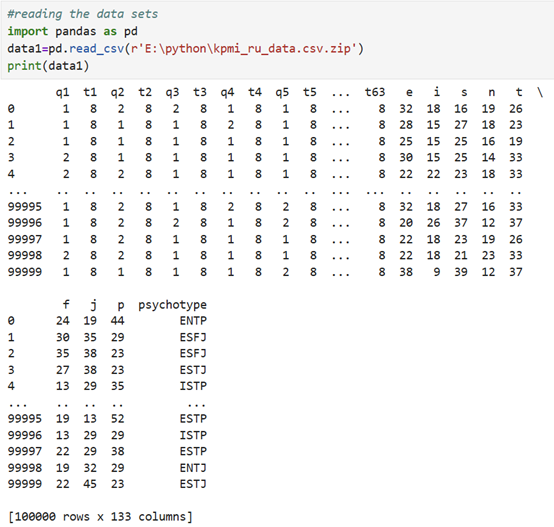
\includegraphics{Q1P1} 
		\caption{Reading KPMIRU Questionnaires Data}
	
	\end{figure}
	\begin{figure}[H]
		\centering
		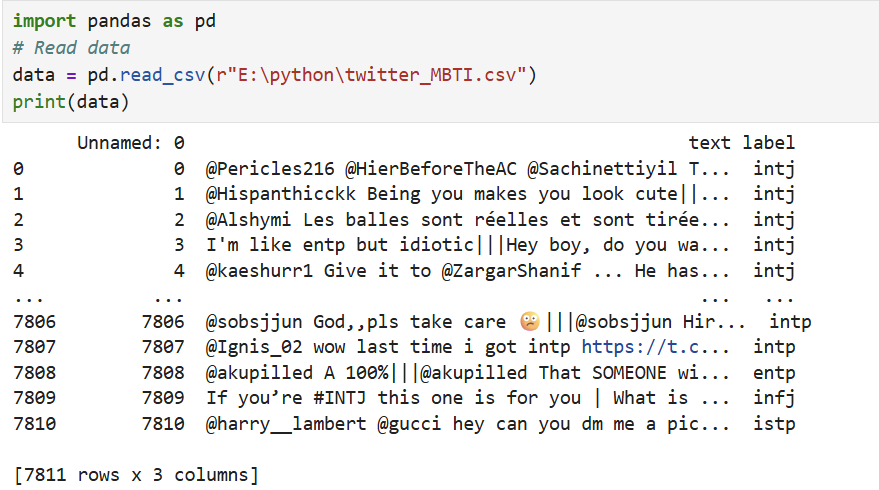
\includegraphics[width=0.9\textwidth]{Q1P2}
		\caption{Reading MBTI Personality Type Twitter Dataset}
	\end{figure}
	As illustrated in the two Figures above, the combined Kaggle sources provide information on:
	\begin{enumerate}
		\item Self-reported MBTI types for each respondent
		\item Raw Twitter posts and basic tweet metadata linked to those MBTI
		labels  
		\item Demographic and psychometric questionnaire answers (KPMIRU survey) 
		\item Behavioral metrics such as posting frequency and topic keywords
		extracted from the tweets
	\end{enumerate}
\section{MBTI in Measurement} 
	\subsection{Data Cleaning and Pre-processing}
	\subsubsection{Handling Missing Values}
	\begin{enumerate}
		\item We use \texttt{dropna()} to eliminate any records with missing or null
		entries. Fortunately, the dataset had no missing psychotype labels or
		scoring data.
		\begin{python}
# Delete null values
df_clean = df.dropna()
		\end{python}
		%e try to change to codeblock style
		% \begin{figure}[H]
		% 	\centering
		% 	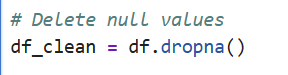
\includegraphics[width=0.9\textwidth]{Q1P4}
			
		% \end{figure}
	\end{enumerate}
\subsubsection{Outlier Detection and Correction}
	\begin{enumerate}
		%e use textbf texttt for better look
		\item Outliers in numeric scores were identified using the \textbf{IQR
		(interquartile range) method}.
		\item For each numeric column, we computed Q1, Q3. IQR = Q3 - Q1
		represent the middle 50\% of the data distribution. The \texttt{lower\_bound} and
		\texttt{upper\_bound} represent the boundaries of the normal range under the
		Interquartile Range Rule (IQR). And then we replaced values outside [Q1
		− 1.5×IQR, Q3 + 1.5×IQR] with the column median. 
		\item The median substitution method mainly serves to stabilize the
		overall distribution and avoid the influence of extreme values.
		\begin{python}
# Select all columns in df_clean with numeric data types (either int or float) in preparation for outlier processing.
numeric_cols = df_clean.select_dtypes(include='number').columns

# Replace the outliers (utilizing the Interquartile Range (IQR) rule) with the median value of the column.
df_processed = df_clean.copy()

for col in numeric_cols:
    Q1 = df_processed[col].quantile(0.25)
    Q3 = df_processed[col].quantile(0.75)
    IQR = Q3 - Q1
    lower_bound = Q1 - 1.5 * IQR
    upper_bound = Q3 + 1.5 * IQR
    median_value = df_processed[col].median()

    # Replace outliers
    df_processed[col] = df_processed[col].apply(lambda x: median_value if x < lower_bound or x > upper_bound else x)
                                           

		\end{python}
	\end{enumerate}
	\subsubsection{Export the cleaned data}
	After completing the outlier replacement and data cleaning process, we used
	df.info() to verify the integrity and structure of the cleaned dataset. The
	cleaned DataFrame was then exported using the \texttt{to\_csv()} method, which saved
	it as \texttt{kpmi\_ru\_data(Cleaned).csv} for downstream analysis. The \texttt{index=False}
	parameter ensured that row indices were not written to the CSV file.
	\begin{python}
print(df_processed.info())
print(df_processed)                                                                                              
df_processed.to_csv(r'E:\python\kpmi_ru_data(Cleaned).csv', index = False) 
	\end{python}
	\begin{figure}[H]
		\centering
		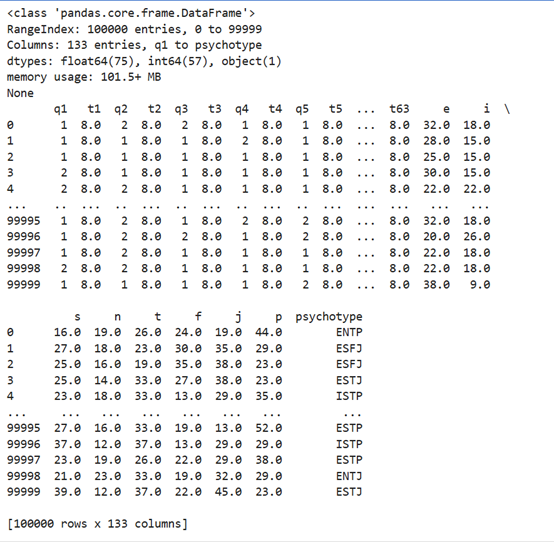
\includegraphics[width=0.9\textwidth]{Q1P7}
		
	\end{figure}
	%e figure number use cref
	The data in the figure 3.1 is the data after our data cleaning.
	
	\subsection{Model Building and Evaluation}
	%e 这一段逻辑要改动
	\textbf{Chi-square test} is an on parametric statistical test to determine if the two
	or more classifications of the samples are independent or
	not \cite{zibran2007chi}. We all know that MBTI has four
	dimensions (Extraversion–Introversion (E–I), Sensing–Intuition (S–N),
	Thinking–Feeling (T–F) and Judging–Perceiving (J–P)). But whether or not
	these four dimensions interrelated or independent of each other stays
	unknown. For explanation, let’s consider the data presented in Figure 3.1 %e cref
	which comprising 100 000 respondents, providing information on the scoring
	fields of the four dimensions of MBTI. In order to find the answer, we use
	the chi-square test.
	
	Each respondent’s type label (e.g., ENTP) was decomposed into its four
	constituent letters, and the sample was cross-classified into a 2 × 2 × 2 ×
	2 contingency table (16 cells)(shown in figure 3.2) %e cref
	\begin{python}
import pandas as pd
import numpy as np
from scipy.stats import chi2

# 1) Read in the cleaned CSV.
FILE_PATH = r"E:\python\kpmi_ru_data(Cleaned).csv"   
df = pd.read_csv(FILE_PATH)

# 2) Extract the columns of four dimensions.(IE, SN, TF, JP)
mbti = df['psychotype'].astype(str).str.upper().dropna()
df_dims = pd.DataFrame({
    'IE': mbti.str[0],   # E 或 I
    'SN': mbti.str[1],   # S 或 N
    'TF': mbti.str[2],   # T 或 F
    'JP': mbti.str[3]    # J 或 P
})

# 3)Construct a 2×2×2×2 contingency table: Obtain the observed frequencies of 16 cells. counts[i,j,k,l]
import pandas as pd
import numpy as np

# Define dimension labels
index = pd.MultiIndex.from_product(
    [['E','I'], ['S','N'], ['T','F'], ['J','P']],
    names=['IE','SN','TF','JP']
)

# Build a DataFrame, using the values of counts as columns.
counts_df = pd.DataFrame({
    'Count': counts.flatten()
}, index=index)

print(counts_df.head(10))
	\end{python}
	%e missing figure
	% \begin{figure}[H]
	% 	\centering
	% 	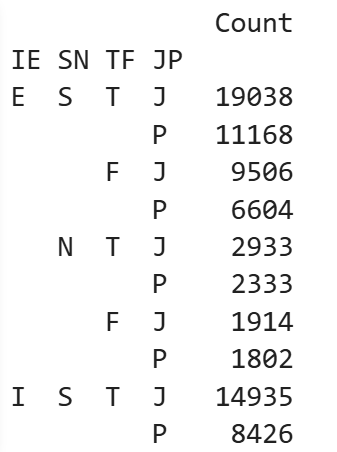
\includegraphics[width=0.5\textwidth]{Q1EDA01} 
	% 	\caption{\centering Decomposed type label}		
	% \end{figure}
	Then we calculate the marginal distribution (the distribution of each
	dimension separately). For example, N\_IE = [count(E), count(I)](shown in
	\cref{fig:Marginaldistribution}) 
	\begin{python}
# Calculate marginal distribution and total number
N_IE = counts.sum(axis=(1,2,3))
N_SN = counts.sum(axis=(0,2,3))
N_TF = counts.sum(axis=(0,1,3))
N_JP = counts.sum(axis=(0,1,2))
N = counts.sum()


marginals = pd.DataFrame({
    'Dimension': ['IE', 'IE', 'SN', 'SN', 'TF', 'TF', 'JP', 'JP'],
    'Category': ['E', 'I', 'S', 'N', 'T', 'F', 'J', 'P'],
    'Count': np.concatenate([N_IE, N_SN, N_TF, N_JP])
})


print(marginals)
	\end{python}
	%e missing figure
	% \begin{figure}[H]
	% 	\centering
	% 	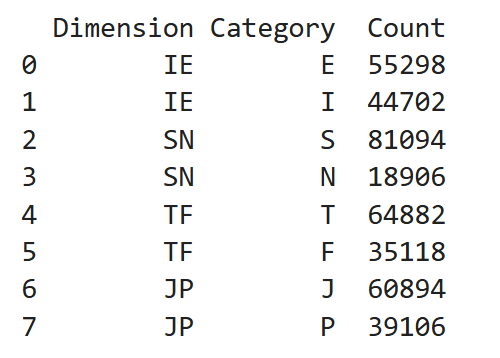
\includegraphics[width=0.9\textwidth]{Q1P09}
	% 	\caption{Marginal distribution}
	% 	\label{fig:Marginaldistribution}
	% \end{figure}
	Under the null hypothesis of mutual independence, the expected frequency in
	each cell was computed as the product of the four one-dimensional marginal
	distributions multiplied by the sample size(shown in \cref{fig:EF}).
	\begin{python}
#Calculate the expected frequency E[i,j,k,l] of each cell based on the completely independent assumption.
E = np.zeros_like(counts, dtype=float)
for i in range(2):
    for j in range(2):
        for k in range(2):
            for l in range(2):
                E[i,j,k,l] = (
                    (N_IE[i]/N) *
                    (N_SN[j]/N) *
                    (N_TF[k]/N) *
                    (N_JP[l]/N)
                ) * N

index = pd.MultiIndex.from_product(
    [['E', 'I'], ['S', 'N'], ['T', 'F'], ['J', 'P']],
    names=['IE', 'SN', 'TF', 'JP']
)

expected_df = pd.DataFrame({
    'Expected_Count': E.flatten()
}, index=index).round(2)

print(expected_df)	
	\end{python}
	% \begin{figure}[H]
	% 	\centering
	% 	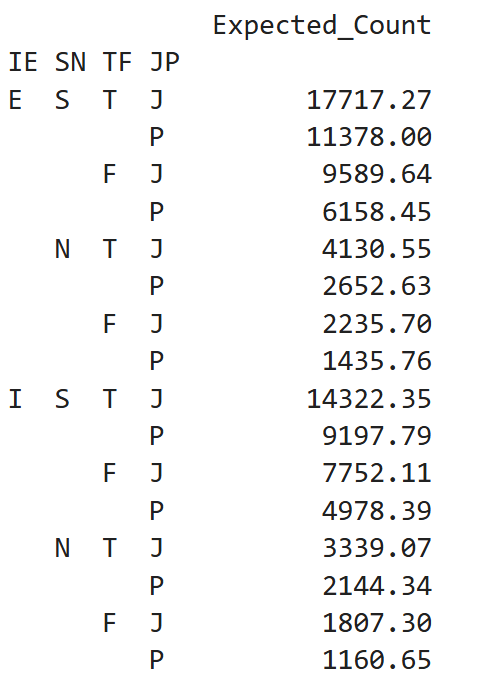
\includegraphics[width=0.9\textwidth]{Q1P010}
	% 	\caption{Expected Frequency}
	% 	\label{fig:EF}
	% \end{figure}

	Now, it’s time to calculate the Pearson chi-square statistic, while $O$ is
	observed value and $E$ is expected value.
	\[
	\chi^2 = \sum \frac{(O - E)^2}{E}
	\]
	\begin{python}
chi2_stat = ((counts - E)**2 / E).sum()
chi2_stat		
	\end{python}
	With this code, we obtain the Pearson chi-square statistic, which is 1342.93063615322.
	
	%e logic change to make the conclusion more clear
	Finally, with $\chi^2 = 1342.93$ and df = 11,we can compute the right - tailed %e df=11?
	probability corresponding to the chi - square statistic under 10 degrees of
	freedom, which is 0. Because the p-value falls far
	below the conventional $\alpha =0.05$ threshold, the null hypothesis is decisively
	rejected: the observed joint distribution of MBTI preferences deviates
	dramatically from what would be expected if the four indices varied
	independently. In practical terms, substantial associations exist among the
	E–I, S–N, T–F and J–P scales, corroborating earlier psychometric critiques
	that the MBTI dimensions are not orthogonal factors but overlap to a
	non-trivial extent. 
	
	Actually, some researchers had also proven that the four
	dimensions of MBTI are not independent. \citeA{fleenor1997relationship}
	investigated the intercorrelations among MBTI continuous scores and found
	that while most dimension pairs demonstrated relatively low correlations,
	the correlation between the Sensing–Intuition (S-N) and Judging–Perceiving
	(J-P) scales was notably higher. Specifically, the study reported a
	correlation coefficient of r = 0.41 between S-N and J-P, indicating a moderate
	positive relationship. This finding has been replicated in other research
	and suggests that individuals who prefer intuition are more likely to also
	prefer perceiving. As such, the assumption of strict statistical
	independence between MBTI preference axes, particularly between S-N and J-P,
	may not hold, which is in line with the findings of our study.
	\begin{python}
df_val = 10
p_val = 1 - chi2.cdf(chi2_stat, df_val)
print(p_val)
if p_val < 0.05:
    print("Conclusion: Reject H₀ —— The four dimensions are not completely independent.")
else:
    print("Conclusion: H₀ cannot be rejected — the four dimensions can be regarded as independent.")

	\end{python}

\subsection{Exploratory Data Analysis (EDA)}
\subsubsection{MBTI Type Frequency}
	\begin{python}
# 2) Frequency bar chart
plt.figure(figsize=(10,4))
df['psychotype'].value_counts().plot(kind='bar')
plt.title('Frequency of 16 MBTI Types')
plt.xticks(rotation=45)
plt.tight_layout()
plt.show()
	\end{python}
	
	A frequency bar chart of the 16 MBTI types was generated using the
	value\_counts() function on the psychotype column. The result was plotted
	using matplotlib and is shown in \cref{mbtidist}.
	%后面需要统一图片命名!!
	%e Can just use \cref{label}
	\begin{figure}[H]
		\centering
		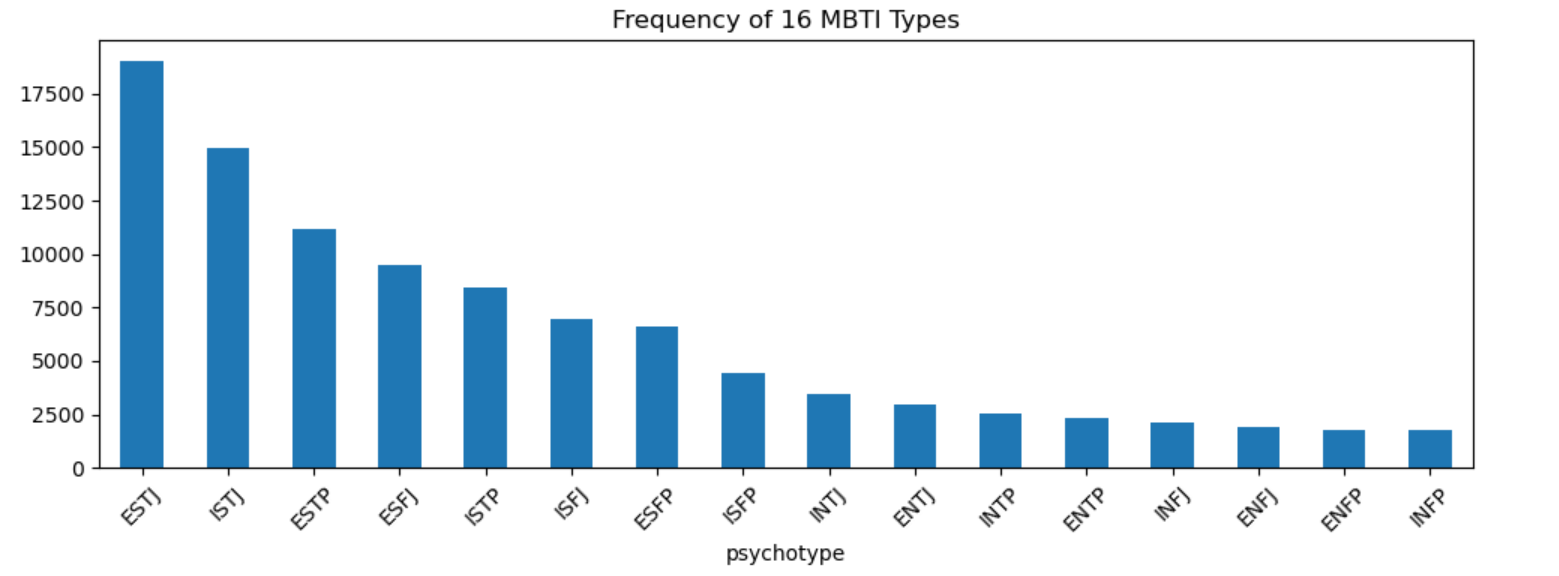
\includegraphics{Q1EDA2} 
		\caption{Frequency of 16 MBTI Types}	
		\label{mbtidist}	
	\end{figure}
	
	As seen in \cref{mbtidist}, the frequency of 16 MBTI types has been shown
	in a descending order. The type ESTJ ranks first, which shows that, based on
	our dataset, the proportion of ESTJ people is the highest. Conversely, the
	proportion of INFP people is the lowest. Additionally, it can be observed
	that the \_S\_J people rankings are relatively high in frequency, as the
	\_NF\_ people rankings are relatively low.
	
	Also, \cref{mbtidist} exhibits severe right oblique imbalance distribution, as
	the number of ESTJ people is nearly 9 times as many as the number of INFP
	people. This phenomenon may be attributed to our database being originally
	from Kaggle, and certain MBTI type tends to participate in such
	investigations.
	
	This contrasts with national MBTI distribution statistics reported in the
	MBTI® Manual, where ISFJ and ESFJ were found to be the most common types
	among U.S. adults (Myers et al., 1998), suggesting that our dataset, to a
	certain extent, fits the population-level trends. In distinct regions, the
	regional differences may influence MBTI type distributions in specific
	rankings.
	
	\subsubsection{Distribution of MBTI Dimension Scores}
	
	\begin{python}
# 3) Histogram of scores in each dimension
score_cols = list('eisntfjp')
df[score_cols].hist(bins=20, figsize=(12,6))
plt.tight_layout()
plt.show()
	\end{python}
	
	Histograms of scores in each MBTI dimension were generated using
	pandas.DataFrame.hist and visualized with matplotlib as shown in \cref{mbtihisto}.
	\begin{figure}[H]
		\centering
		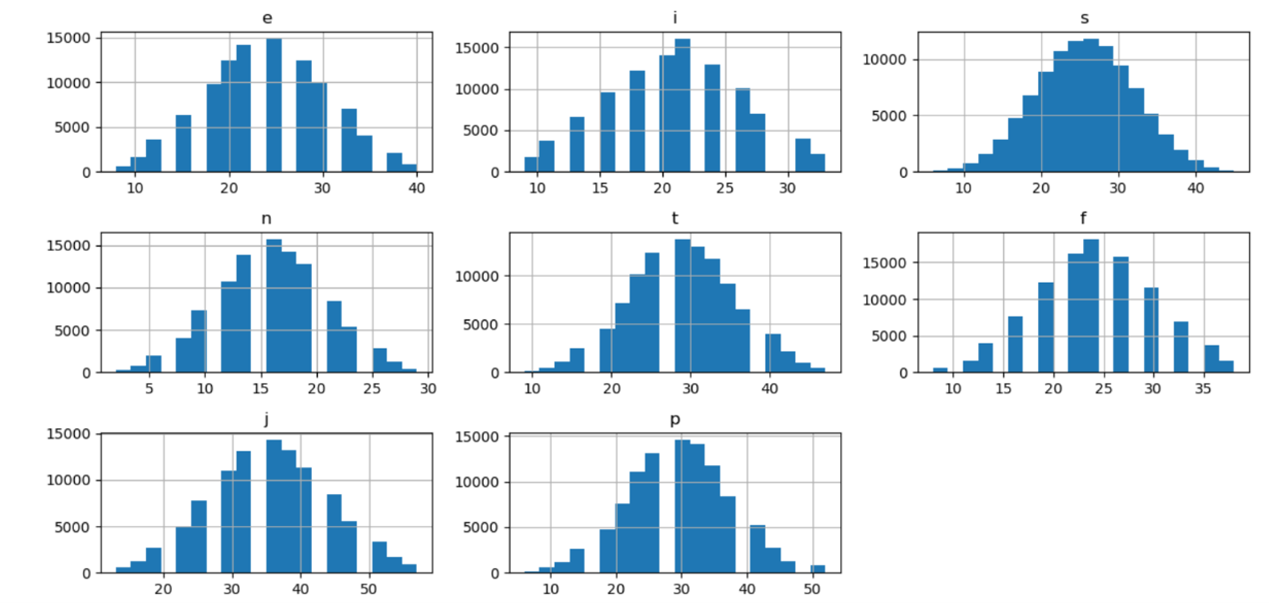
\includegraphics{Q1EDA4} 
		\caption{Histogram of MBTI Dimension Scores}
		\label{mbtihisto}		
	\end{figure}
	
	As seen in \cref{mbtihisto}, from the score concentration trend, the eight
	MBTI poles vary in concentration. For example, E, S, and T scores are
	generally spread from 10 to 40, while N and I scores are more narrowly
	concentrated between 5 to 30. And in detail, in the dimension of P and T,
	exhibit higher scores, which shows the preference toward Thinking and
	Perceiving. Compared to them, in the dimension of N and I, they exhibit
	lower scores, which indicates most people are more inclined toward
	Extraversion and Sensing.
	%e 这里要补上双峰分布的说明!
	From the data obtained from these diagrams, we can observe that most samples
	in these dimensions show distributional asymmetries, as not evenly
	distributed. Particularly for the high values of J and low values of N, this
	result matches the observation at 4.1.1 that \_S\_J types dominate the %e cref 4.1.1
	database.
	
\subsubsection{Descriptive Statistics of MBTI Dimensions}
	\begin{python}
# 4) Describe statistics (mean, std, quartile, skewness, kurtosis)
stats = df[score_cols].describe().T
stats['skew']  = df[score_cols].skew()
stats['kurt']  = df[score_cols].kurt()
print(stats.round(2))
	\end{python}
	

	
	Descriptive statistics of each MBTI dimension were computed and consolidated
	into a single summary table, including skewness and kurtosis, to facilitate
	score distribution analysis shown in \cref{descstatmbti}.
	
	\begin{figure}[H]
		\centering
		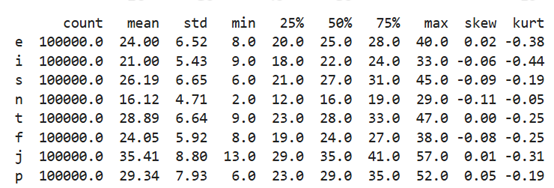
\includegraphics{Q1EDA6} 
		\caption{Descriptive Statistics of MBTI Dimension Scores}	
		\label{descstatmbti}	
	\end{figure}
	
	%还有交叉引用要改(不过是不是不改也行?	
	Based on Table 4.1.3, it can be observed that the dimensions of I, S, N, and %e cref
	F showcase a notable positive skew distribution, as the dimension of N, with
	a value of -0.11, demonstrates left skewness most. This phenomenon tends to
	show that most people are more likely to be Sensing(S) and so on. And in
	contrast, the dimension of P with the value of +0.05 exhibits right
	skewness, implying a preference towards lower values, showing that
	Judging(J) dominates more in this database. Results of these also support
	the conclusion in Figure 4.1.1 that \_S\_J people occupy the majority. %e cref
	
	And from the kurtosis value, it can be seen that most values are around 0
	and negative, which suggests that all the dimension is distributed
	platykurtic. With relatively concentrated values, this exhibits the loss of
	extreme outliers. Also, the maximum value and minimum value that all
	dimensions have can be used in the form of Max-Min, which demonstrates that
	J and P dimensions have the largest difference, indicating that individual
	differences between them are the strongest.
	\begin{figure}[H]
		\centering
		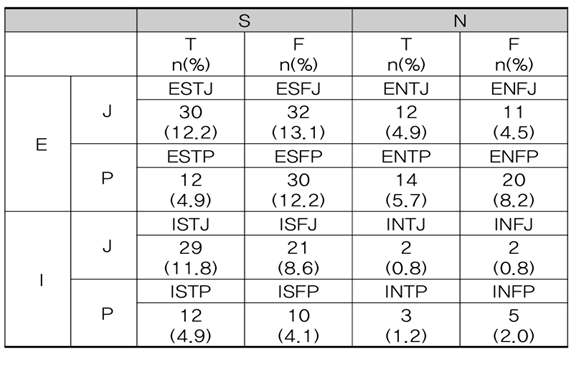
\includegraphics{Q1EDA7} 
		\caption{MBTI Distribution of 16 Personality Types}		
	\end{figure}
	
	Figure 4.1.3 MBTI Distribution of 16 Personality Types from Jang and Kim %e cref
	(2014), supporting the dominance of \_S\_J types observed in our dataset. 
	
\subsubsection{Correlation Analysis Between MBTI Dimensions}
	\begin{python}
# 5) Correlation matrix heat map
plt.figure(figsize=(6,5))
sns.heatmap(df[score_cols].corr(), annot=True, cmap='coolwarm')
plt.title('Correlation between dimension scores')
plt.tight_layout()
plt.show()
	\end{python}
	A Pearson correlation heatmap was constructed to visualize linear
	relationships among MBTI dimension scores, as shown in \cref{personheatmap}.
	\begin{figure}[H]
		\centering
		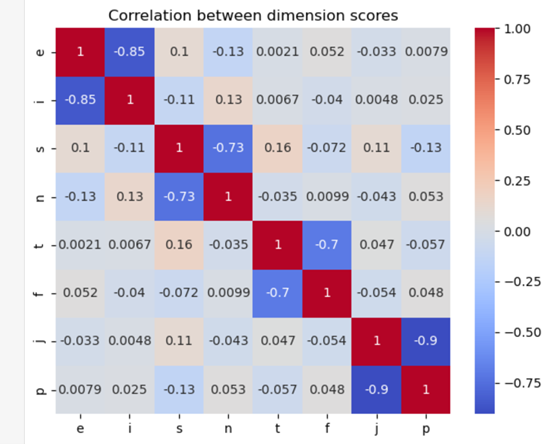
\includegraphics{Q1EDA9} 
		\caption{Correlation Heatmap of MBTI Dimension Scores}	
		\label{personheatmap}	
	\end{figure}
	
	As seen in \cref{personheatmap}, the correlation between the opposite
	dimensions, like E vs I, S vs N, T vs F, and J vs P. All of them are
	strongly negative, which is consistent with the design concept of MBTI, as
	the two poles of each dimension are opposed. As a result, the MBTI method
	has its rationality. This result aligns with (Li et al., 2024), who also %e Invaild Reference!!
	observed that “the correlations between the four axes are generally weak,
	indicating that the personality traits on each axis are relatively
	independent” (p. 12).% better use \cite
	
	Furthermore, in \cref{personheatmap}, the correlation between other dimension pairs
	is low (nearly 0). This phenomenon supports that the dimensions are
	seemingly independent. While the correlation between S and T is +0.16, a bit
	larger than others, it indicates that someone who is Sensing(S) tends to be
	Thinking(T). In contrast, the correlation between S and P is -0.13, which
	indicates that those who are Sensing(S) tend to be Judging(J).
	%e先综述主题建模是什么——》数据清洗步骤必要性解释,结果展示-》主题建模步骤
	%e-》EDA
	%eintro需要解释objective的原因,将文章分为两个分析方向,解释两者之间的联系;MBTI的进一步解释有必要,写什么根据我后面EDA决定
\section{MBTI in Manifestation} 
	In the previous section, we examined the statistical characteristics of
	MBTI. In this section, we turn to the manifestation level by investigating
	how different MBTI types vary in their topic preferences and expressive
	patterns on Twitter.	
	
	\subsection{Topic Preferences of MBTI Personalities}
	To analyze the topic preference of different MBTI personalities, we adopt
	\textbf{LDA modeling}.
	
	\textbf{Latent Dirichlet Allocation} (LDA) is a generative probabilistic model for
	uncovering hidden “topics” in a large collection of documents. It assumes
	each document is composed of a mixture of topics, and each topic is
	represented by a distribution over words. For example, a document might be
	30\% about "technology" and 70\% about "health", with each topic associated
	with its own common vocabulary.
	
	In the LDA framework, the generation of a document is imagined as a two-step
	process:
	\begin{enumerate}
		\item a topic distribution is assigned to the document.
		\item For each word in the document:
		\begin{itemize}
			\item A topic is randomly chosen based on the document’s topic distribution.
			\item A word is selected from the vocabulary of that topic.
		\end{itemize}
	\end{enumerate}
	During model training, this generative process is reversed: LDA infers the
	underlying topic structure based on the observed words in the documents. It
	estimates:
	\begin{itemize}
		\item the topic proportions for each document
		\item the most representative words for each topic
	\end{itemize}
	
	The specific LDA process of our project will be discussed in detail.
	However, LDA model has a extremely high requirement for text data cleaning,
	since LDA relies on word‐frequency patterns to infer
	hidden topics. It’s important to remove noise, such as words that are
	meaningless or unrepresentative, so that the model can produce reliable topics.
	Thus, we need to make sure our dataset is clean and ready
	for LDA modeling. 
	%e logic can be changed
\subsubsection{Data Cleaning}
Because of the nature of the project, we must work with a dataset that contains a large volume of text. The raw dataset we obtained suffers from the following issues:
\begin{enumerate}
\item Text granularity / structure: In each row, the posts field actually concatenates 50 posts from a single user, separated by "|||".
\item Dirty characters and encoding: The data contain URLs, HTML fragments, escape sequences, and leading single quotation marks.
\item Length and memory footprint: Each row is about 7 k characters on average, with some rows exceeding 10 k characters.

\end{enumerate}
These problems prevent the dataset from being used directly for analysis, so we must clean it first.
%这里没法加4级标题了,需修改语言
Importing Modules and the Dataset
\begin{enumerate}
\item Import the required library
\begin{python}
import pandas as pd
\end{python}
This line imports the pandas library under the alias pd. Pandas is a powerful tool for data analysis and manipulation, especially well suited for reading and processing structured data such as CSV files.
\item Import N analyze data p1 LP related modules
\begin{python}
import re, string
from typing import List
import nltk
from nltk.tokenize import word_tokenize
from nltk.corpus import stopwords, wordnet
from nltk import pos_tag
from nltk.stem import WordNetLemmatizer

\end{python}

These statements import several NLP utilities:
\begin{itemize}
\item re, string: regular expression and character utilities for text processing.
\item typing.List: type annotation for list data structures.
\item The nltk suite: tokenisation (word\_tokenize), stop word handling (stopwords), part of speech tagging (pos\_tag), lemmatisation (WordNetLemmatizer), and more.
\end{itemize}
\begin{python}
my_nltk_path = "Data"
nltk.data.path.append(my_nltk_path)

\end{python}
This sets the local NLTK resource path to the Data directory and appends it to the search path so that NLTK can load the required resources in the local environment.
\begin{python}
import textstat
from vaderSentiment.vaderSentiment import SentimentIntensityAnalyzer

\end{python}
\begin{itemize}
\item textstat: assesses text readability.
\item SentimentIntensityAnalyzer: VADER’s sentiment analysis tool for assessing the affective polarity of text.
\end{itemize}
\item Import modules for reading and writing external files
\begin{python}
import json
import pickle
import copy

\end{python}
\begin{itemize}
\item json: parsing and serialising JSON data.
\item pickle: serialising and deserialising Python objects.
\item copy: making shallow and deep copies of objects.
\end{itemize}

\item Load the FastText language identification model
\begin{python}
import fasttext
lang_model = fasttext.load_model("lid.176.bin")

\end{python}
This loads Facebook’s FastText model lid.176.bin, which recognises 176 languages and returns language codes (e.g. "en", "zh", "es"). It is essential when pre processing multilingual data—especially when we need to standardise text to English via translation.

\item Load a local large language model (LLM) and specify the model version
\begin{python}
import ollama
llm = "llama3.1:8b"

\end{python}
ollama provides an interface for running LLMs locally. Here we call the LLaMA 3 model with 8 billion parameters, a lightweight model used for on premise translation to improve privacy and efficiency when translating large corpora offline.
\item Bring in the tqdm progress bar and enable Pandas integration
\begin{python}
from tqdm.auto import tqdm
tqdm.pandas()

\end{python}
TQDM is a popular Python progress bar library. tqdm.auto selects the most suitable display backend automatically (Jupyter friendly). Calling tqdm.pandas() enables progress bars for DataFrame.apply() and Series.apply() operations, giving real time feedback during long running tasks.
\item Define an average value helper
\begin{python}
def ave(1):
    return sum(1) / len(1)

\end{python}
A simple function ave is defined to calculate the average of a list of numeric values.

\item Define the list of MBTI personality types
\begin{python}
MBTI_types = [
    "ISTJ", "ISFJ", "INFJ", "INTJ",
    "ISTP", "ISFP", "INFP", "INTP",
    "ESTP", "ESFP", "ENFP", "ENTP",
    "ESTJ", "ESFJ", "ENFJ", "ENTJ"
]

\end{python}
A list named MBTI\_types is defined, containing all 16 Myers-Briggs personality types, to serve as the classification basis in subsequent text or label processing.

\item Read the data and perform an initial split
\begin{python}
raw_data = pd.read_csv("Data\\twitter_MBTI.csv", encoding="utf-8")
raw_data.drop(columns="Unnamed: 0", inplace=True)
raw_data.columns = ["posts", "type"]

for i in raw_data.index:
    temp = raw_data.loc[i, "posts"]
    temp = temp.split("|||")
    raw_data.loc[i, "posts"] = temp

\end{python}
First, the CSV file twitter\_MBTI\.csv is loaded into a DataFrame. The automatically added index column ("Unnamed: 0") is removed, and the columns are renamed to standardise their labels. Each row’s posts field is then split on the delimiter "|||", converting the concatenated string into a list of separate posts for subsequent sentence level analysis.

\item Load and merge the custom stop word list
\begin{python}
from custom_stopwords import custom_stopwords
stop_words.update(custom_stopwords)

\end{python}
custom\_stopwords is a task specific collection of terms—such as social media jargon ("lol", "omg", "http"), MBTI irrelevant proper nouns, or noise tokens—that should be excluded. Merging it into stop\_words ensures these words are filtered out during cleaning.

\end{enumerate}

Methods for Data Cleaning 
\begin{enumerate}
\item Loading the contraction mapping
\begin{python}
with open(file="contractions.json", mode='r', encoding='utf-8') as f:
    contractions_map = json.load(f)

\end{python}
contractions.json maps common English contractions to their full forms (e.g. "don't" → "do not"), facilitating normalisation of user‑generated content.
\item Constructor \_\_init\_\_
\begin{python}
def __init__(self, source=raw_data):
    self.data = source

\end{python}
Initialises the object with a DataFrame that contains a posts column in which each entry is a list of sentences.
\item Remove user mentions and hashtags
\begin{python}
def remove_mention_and_tag(self):
    def process_removal(post):
        post_without_mention=[]
        for sentence in post:
            # Use re to scan and substitute
            post_without_mention.append(
                re.sub(
                    pattern=r'@\w+|#\w+',
                    repl=' ',
                    string=sentence
                )
            )
        return post_without_mention
    self.data["posts"]=self.data["posts"].apply(process_removal)

\end{python}
This method defines an inner function \texttt{process\_removal} that scans each sentence in a post with the regular expression \texttt{r'@\textbackslash w+|\#\textbackslash w+'} and replaces every mention or hashtag with a space, thereby stripping social media tags while preserving sentence order. The \texttt{apply()} call performs this operation on the entire \texttt{posts} column.

\item Delete URL hyperlinks
\begin{python}
def remove_url(self):
    def process_remove_url(post):
        post_without_url = []
        for sentence in post:
            post_without_url.append(
                re.sub(
                    pattern=r'http\S+|www\S+|https\S+',
                    repl='',
                    string=sentence,
                    flags=re.MULTILINE
                )
            )
        return post_without_url
    self.data["posts"] = self.data["posts"].apply(process_remove_url)

\end{python}
The method removes any web page address (e.g. http://…, www.…), preventing links from contaminating downstream text analysis.

\item Strip emoji characters
\begin{python}
    def remove_emoji(self):
        def process_remove_emoji(post):
            post_without_emoji=[]
            for sentence in post:
                # Use re to scan and substitute
                emoji_pattern=re.compile(
        "["
        "\U0001F600-\U0001F64F"  # Emoticons
        "\U0001F300-\U0001F5FF"  # Miscellaneous Symbols and Pictographs
        "\U0001F680-\U0001F6FF"  # Transport and Map Symbols
        "\U0001F1E0-\U0001F1FF"  # Flags (iOS)
        "\U00002702-\U000027B0"  # Dingbats
        "\U000024C2-\U0001F251"  # Enclosed Characters, etc.
        "\U0001f926-\U0001f937"  # Supplemental Symbols and Pictographs
        "\U00010000-\U0010ffff"  # Broader range for some less common emojis
        "]+", flags=re.UNICODE
                )

\end{python}

The regular expression spans multiple Unicode ranges—covering most common and uncommon emojis such as facial expressions, gestures, vehicles, map icons, a wide variety of regional flags and pictographic symbols, and even supplementary characters beyond the Basic Multilingual Plane (BMP)—with flags=re.UNICODE enabled to ensure all Unicode characters are recognized.
\begin{python}
                post_without_emoji.append(
                    emoji_pattern.sub(
                        repl=' ',
                        string=sentence
                    )
                )
            return post_without_emoji
        self.data["posts"]=self.data["posts"].apply(process_remove_emoji)

\end{python}
For each sentence, the regex matches emojis and replaces every matched character with a single space (' '), preventing token concatenation noise while maintaining readability and analyzability; the process\_remove\_emoji function is then applied to the entire posts column via .apply(), bulk-removing emojis from every post and overwriting the original data column with the cleaned results.
\item Expand English contractions

Static method text\_expand()
\begin{python}
@staticmethod
def text_expand(original_string, contraction_mapping=contractions_map):
\end{python}

Defines a static method \texttt{text\_expand()} that takes a single string (a
sentence) as input and, by default, uses the pre-loaded dictionary of
contractions \texttt{contractions\_map} to convert contractions to their full
forms.

\begin{python}
contractions_pattern = re.compile('({})'.format('|'.join(contraction_mapping.keys())), flags=re.IGNORECASE | re.DOTALL)
\end{python}

This statement concatenates all the keys (i.e., every contraction) in the
mapping dictionary into a regular expression pattern so that any occurrence of
a contraction in the text can be captured. The flag \texttt{re.IGNORECASE}
makes the match case insensitive, and \texttt{re.DOTALL} allows the pattern to
span across line breaks.

\begin{python}
def text_mapping(text_matched):
    old_text = text_matched.group(0)
    new_text = contraction_mapping.get(old_text.lower())
    if not new_text:
        new_text = contraction_mapping.get(old_text)
        if not new_text:
            return old_text
    return new_text
\end{python}

The inner function \texttt{text\_mapping()} replaces each matched contraction
with its full form. It first tries to match the lowercase version; if that
fails, it tries the original case. If a replacement still cannot be found, it
returns the original text unchanged, preventing information loss.

\begin{python}
expanded_string = contractions_pattern.sub(repl=lambda m: text_mapping(m), string=original_string)
return expanded_string
\end{python}

Using \texttt{re.sub()}, every match in the original string is replaced, and
the expanded string is finally returned.

%------------ Method expand_contractions() --------------------------------
\begin{python}
def expand_contractions(self):
    def process_expand_contractions(original_list):
        for idx in range(len(original_list)):
            original_list[idx] = Data_to_Clean.text_expand(original_list[idx])
        return original_list
    self.data["posts"] = self.data["posts"].apply(lambda x: process_expand_contractions(x))
\end{python}

This method batch-processes every \texttt{posts} entry in the DataFrame. Each
\texttt{posts} entry is a list of strings, representing multiple sentences
written by a user. The nested function \texttt{process\_expand\_contractions()}
calls the static method \texttt{text\_expand()} on every sentence in the list,
expanding all contractions to their full forms.  
Finally, \texttt{apply()} is used to apply the processing to the entire column,
achieving large-scale contraction expansion. This greatly improves the
consistency and semantic clarity of the data, which benefits subsequent
tokenization, vectorization, and modelling stages.

%------------ 7. Convert to lower case ------------------------------------
\begin{python}
def tolower(self):
    def process_tolower(post):
        return [sentence.lower() for sentence in post]
    self.data["posts"] = self.data["posts"].apply(process_tolower)
\end{python}

Uniform lower casing prevents word-frequency fragmentation due to case
differences.

%------------ 8. Remove punctuation ---------------------------------------
\begin{python}
def remove_punct(self):
    def process_remove_punct(post):
        post_without_punct = []
        for sentence in post:
            post_without_punct.append(
                re.sub(pattern=r'[^a-zA-Z\s]', repl=' ', string=sentence)
            )
        return post_without_punct
    self.data["posts"] = self.data["posts"].apply(process_remove_punct)
\end{python}

Non-alphabetic characters are replaced by spaces, simplifying the text for
language modelling.

%------------ 9. Delete blank strings -------------------------------------
\begin{python}
def remove_whitespace(self):
    def process_remove_whitespace(post):
        return [sentence for sentence in post if sentence.strip()]
    self.data["posts"] = self.data["posts"].apply(process_remove_whitespace)
\end{python}

Sentences that are empty or contain only whitespace are discarded.

%------------ 10. Tokenization --------------------------------------------
\begin{python}
def totokens(self):
    def process_totokens(post):
        post_totokens = []
        for sentence in post:
            tokens = word_tokenize(sentence)
            post_totokens.append(tokens)
        return post_totokens
    self.data["posts"] = self.data["posts"].apply(process_totokens)
\end{python}

\texttt{word\_tokenize()} splits each cleaned sentence into a list of tokens,
providing the basic units for further NLP tasks.

%------------ 11. Remove stop-words ---------------------------------------
\begin{python}
def remove_stopwords(self):
    def process_remove_stopwords(post):
        stop_words = set(stopwords.words("english"))
        filtered_post = []
        for sentence in post:
            filtered_sentence = [word for word in sentence if word not in stop_words]
            filtered_post.append(filtered_sentence)
        return filtered_post
    self.data["posts"] = self.data["posts"].apply(process_remove_stopwords)
\end{python}

Common high-frequency, low-information words are filtered out to emphasise
lexical content relevant for modelling.

%------------ 12. Lemmatize -----------------------------------------------
\begin{python}
def post_lemmatize(self):
    def process_lemmatize(post):
        def get_wordnet_postag(old_postag):
            if old_postag.startswith('J'): return wordnet.ADJ
            elif old_postag.startswith('V'): return wordnet.VERB
            elif old_postag.startswith('N'): return wordnet.NOUN
            elif old_postag.startswith('R'): return wordnet.ADV
            else: return wordnet.NOUN

        lemmatizer = WordNetLemmatizer()
        lemmatized_post = []
        for tokens in post:
            tagged_tokens = pos_tag(tokens)
            lemmatized_tokens = [lemmatizer.lemmatize(word, get_wordnet_postag(tag)) for word, tag in tagged_tokens]
            lemmatized_post.append(lemmatized_tokens)
        return lemmatized_post
    self.data["posts"] = self.data["posts"].apply(process_lemmatize)
\end{python}

Words are reduced to their dictionary forms based on POS tags, decreasing
dimensionality and unifying inflected variants.

%------------ 13. Drop empty sentences ------------------------------------
\begin{python}
def drop_empty(self):
        def process_drop(post):
            result=[sentence for sentence in post if sentence!=[]]
            return result        
        self.data["posts"]=self.data["posts"].apply(process_drop)
\end{python}

After cleaning, residual empty sentences are removed to maintain structural
integrity.


\end{enumerate}

%这步之前我放在LDA里面了这后面放哪你看看
%%%%%%%%%%%%%%%%%%%%%%%%%%%%%%%%%%%%%%%%%%%%%%%%%%%%%%%%%%%%%%%%%%%%%%%%%%%%
%  Workflow (continued): Steps 8–10
%%%%%%%%%%%%%%%%%%%%%%%%%%%%%%%%%%%%%%%%%%%%%%%%%%%%%%%%%%%%%%%%%%%%%%%%%%%%

\setcounter{enumi}{7} % continue numbering from previous list (step 7 ended)

\begin{enumerate}
%---------------------------------------------------------------------------
\item \textbf{Automatically Detect Non-English Sentences}

\begin{python}
def locate_str_to_translate(self):
    result = []
    for i in tqdm(self.data.index,
                  desc="Locating strings of other languages..."):
        for j in range(len(self.data.loc[i, "posts"])):
            sentence = self.data.loc[i, "posts"][j]

            # Only check sentences longer than eight words
            if len(sentence.split()) > 8:
                lang_prediction = lang_model.predict(
                    re.sub(r'\s+', ' ', sentence).strip(),
                    k=1                             # top-1 prediction
                )

                # Keep if not English & confidence > 0.98
                if (lang_prediction[0][0] != "__label__en"
                        and lang_prediction[0][1] > 0.98):
                    result.append(
                        (i, j,
                         re.sub(pattern=r"__\w+__",
                                repl='',
                                string=lang_prediction[0][0]))
                    )

    self.locations = result
    with open(f"Data/{self.basic_identities['type']}_translate_location.pkl",
              "wb") as f:
        pickle.dump(result, f)
\end{python}

\begin{itemize}
  \item \textbf{Outer loop}: iterates over the entire DataFrame index, visiting each post sequentially.
  \item \textbf{Inner loop}: traverses every sentence inside the current post (a list of sentences).
  \item \textbf{tqdm} renders a progress bar for large-scale datasets.
  \item A lower bound of \texttt{> 8} words avoids language-detection errors on extremely short sentences.
  \item The FastText model returns a tuple \texttt{('\_\_label\_\_xx', confidence)}; only non-English predictions with confidence \texttt{>} \texttt{0.98} are stored.
  \item Results are saved both in \texttt{self.locations} and pickled to disk for later translation.
\end{itemize}

%---------------------------------------------------------------------------
\item \textbf{Translate with a Local LLM}

\begin{python}
def translate_str(self):
    for coord in tqdm(self.locations,
                      desc="Translating string into English..."):
        sentence = self.data.loc[coord[0], "posts"][coord[1]]

        self.data.loc[coord[0], "posts"][coord[1]] = \
            ollama.generate(
                model=llm,
                prompt=(
                    f"Translate from {coord[2]} to English: \"{sentence}\"\n"
                    f"Output ONLY the translated text."
                )
            )['response']
\end{python}

Each non-English sentence identified in Step 8 is translated \emph{in place}
by a locally hosted LLM (e.g.\ \texttt{llama3.1:8b}).  
The prompt specifies the source language and requests only the English
rendition, preserving post order and structure.

%---------------------------------------------------------------------------
\item \textbf{Filter Non-English Sentences by Language ID}

\begin{python}
def process_drop(post, level=0.98):
    filtered_post = []
    for sentence in post:
        norm = re.sub(r"\s+", " ", sentence)

        # Keep very short sentences to avoid false negatives
        if len(norm.split()) < 6:
            filtered_post.append(norm)
            continue

        lang = lang_model.predict(norm)
        if lang[0][0] == '__label__en' and lang[0][1] > level:
            filtered_post.append(norm)
        else:
            # Retry in lowercase for robustness
            lang = lang_model.predict(norm.lower())
            if lang[0][0] == '__label__en' and lang[0][1] > level:
                filtered_post.append(norm)
    return filtered_post

self.data["posts"] = self.data["posts"].apply(process_drop)
\end{python}

\begin{itemize}
  \item Filters out non-English sentences without translating them.
  \item Sentences shorter than six words are retained to reduce false negatives.
  \item Longer sentences must pass an English-confidence threshold
        (\texttt{level}, default \texttt{0.98}).
  \item A second check on the lowercase version mitigates errors from mixed
        casing or acronyms.
\end{itemize}

\end{enumerate}


Create a data processing method that encompasses the entire workflow
\begin{enumerate}
%---------------------------------------------------------------------------
\item \textbf{Initialize the Data Object \& Remove URLs}

\begin{python}
data = Data_to_Analyze(type=TYPE)
data.remove_url()
data.remove_mention_and_tag()
\end{python}

\begin{itemize}
  \item Instantiate a \texttt{Data\_to\_Analyze} object to load the raw dataset for the specified personality type \texttt{TYPE}.
  \item Call \texttt{remove\_url()} and \texttt{remove\_mention\_and\_tag()} to strip out hyperlinks, user mentions (\texttt{@username}), and topic hashtags (\texttt{\#topic}), eliminating social-media noise.
\end{itemize}

%---------------------------------------------------------------------------
\item \textbf{Extract Structured Text Features (Before Cleaning)}

\begin{python}
data.get_sentence_quantity()
data.get_word_count()
data.get_upper_ratio()
data.get_readability()
data.get_vader_score()
\end{python}

\begin{itemize}
  \item \texttt{get\_sentence\_quantity()} – counts the number of sentences in each post.
  \item \texttt{get\_word\_count()} – totals the words in each post.
  \item \texttt{get\_upper\_ratio()} – computes the ratio of uppercase letters to all alphabetic characters.
  \item \texttt{get\_readability()} – evaluates readability using two \texttt{textstat} metrics: Flesch Reading Ease and Gunning Fog Index.
  \item \texttt{get\_vader\_score()} – applies the VADER model for sentiment analysis, yielding composite sentiment scores.
\end{itemize}

\textbf{Important:} Run these functions \emph{before} any cleaning steps such as contraction expansion or case conversion, since those operations alter the statistics.

%---------------------------------------------------------------------------
\item \textbf{Continue Text-Cleaning Tasks}

\begin{python}
data.remove_emoji()
data.remove_whitespace()
data.drop_non_english(0.75)
data.expand_contractions()
data.tolower()
data.remove_punct()
data.remove_whitespace()
data.totokens()
\end{python}

\begin{itemize}
  \item \texttt{remove\_emoji()} – removes emoji and other non-text graphical elements.
  \item \texttt{remove\_whitespace()} (first pass) – performs an initial whitespace cleanup.
  \item \texttt{drop\_non\_english(0.75)} – uses fastText to detect language and drops sentences that are not English when confidence is below \texttt{0.75}.
  \item \texttt{expand\_contractions()} – expands English contractions (e.g., ``don’t'' $\rightarrow$ ``do not'').
  \item \texttt{tolower()} – converts all text to lowercase, reducing word-form variability.
  \item \texttt{remove\_punct()} – strips punctuation to facilitate vectorization or model processing.
  \item \texttt{remove\_whitespace()} (second pass) – clears residual extra spaces from earlier steps.
  \item \texttt{totokens()} – tokenizes the cleaned sentences into word lists (tokens) for downstream vectorization or language-model tasks.
\end{itemize}

%---------------------------------------------------------------------------
\item \textbf{Persist the Cleaned Data as a Binary File}

\begin{python}
with open(f"Data\\cleaned_data\\{TYPE}_cleaned.pkl", "wb") as f:
    pickle.dump(data, f)
\end{python}

Serializes the cleaned data object to disk in binary format with \texttt{pickle}, enabling rapid reuse for model training or further analysis.

%---------------------------------------------------------------------------
\item \textbf{Run the Analysis in Batch for All MBTI Types}

\begin{python}
for T in tqdm(MBTI_types):
    analyze_data_p1(T)
\end{python}

Iterates over \texttt{MBTI\_types} (assumed to include all 16 personality types) and executes \texttt{analyze\_data\_p1()} for each one, enabling efficient, consistent batch processing across the entire dataset.
\end{enumerate}

















\subsubsection{LDA modeling}
	The cleaned data are organized by MBTI types, each as a tokenized and
	preprocessed text collection stored in a structured \texttt{pd.DataFrame}. 
	%e sentence above can be removed or refined
	To perform LDA modeling, the input must be converted into a
	\textbf{Bag-of-Words (BoW) corpus}, where each document is represented as a
	list of (word\_id, frequency) tuples. This requires mapping each unique word
	to a distinct integer ID, resulting in a \textbf{dictionary} that captures
	the vocabulary of the entire corpus. In this assignment, we apply filtering
	by removing words that appear in more than 20\% of documents
	(\texttt{no\_above=0.2}) and those that appear in fewer than 50 documents
	(\texttt{no\_below=50}) to retain only representative terms.
	%e change logic
	\begin{python}
import gensim.corpora as corpora
from gensim.models import CoherenceModel
def constract_initial_dict(source,no_above,no_below):

    output = {T: {
        "original_text": [],
    } for T in MBTI_types}
    
    output["all_original_text"]=[]
    for T in tqdm(MBTI_types):
        for i in source[T].data.index:
            temp=source[T].data.loc[i,"posts"]
            output[T]["original_text"].append(temp)
        output["all_original_text"].extend(output[T]["original_text"])
    output["overall_dict"]=corpora.Dictionary(output["all_original_text"])
    output["overall_dict"].filter_extremes(no_above=no_above,no_below=no_below)
    output["overall_dict"].compactify()
    print("Size of dictionary:",len(output["overall_dict"]))
    output["all_corpus"]=[output["overall_dict"].doc2bow(post_token) for post_token in output["all_original_text"]]
    return output
initial_dict=constract_initial_dict(source=cleaned_data,
                                    no_above=0.20,
                                    no_below=50)
with open("Data/initial_dict.pkl",'wb') as f:
    pickle.dump(initial_dict,f)
	\end{python}
	
	For a convenient inspection, we computed the overall term‐frequency
	distribution by summing each token’s bag‐of‐words counts across the entire
	corpus and stored the result table as a CSV file:
	\begin{python}
def check_corpus(corpus,dict,name=''):
    result=pd.DataFrame(
        [
            list(range(len(dict))),
            [0]*len(dict)
        ]
    ).T
    result.columns=["word","frequency"]
    for post in tqdm(corpus):
        for word_tuple in post:
            result.loc[word_tuple[0],"frequency"]+=word_tuple[1]
    for i in result.index:
        result.loc[i,"word"]=dict[i]
    result=result.sort_values(by="frequency",ascending=False)
    result.to_csv(f"Data/{name}id2word_result.csv")
	\end{python}
	
	Selecting an appropriate number of topics is crucial for LDA modeling. If
	the topic number is too small, unrelated content may be merged into the same
	topic, reducing modelinterpretability. Conversely, an excessively large number of
	topics may fragment coherent semantic themes, leading to redundancy and
	overlap among topics. To determine the optimal number of topics for the LDA
	model, we will first train several temporary LDA models (\texttt{temp\_lda\_model}) with different
	numbers of topics. The semantic coherence and interpretability of the
	resulting topics were evaluated using the c\_v coherence score, which
	measures how consistently related the top words within each topic are. 
	\begin{python}
with open("Data/initial_dict.pkl","rb") as f:
    initial_dict=pickle.load(f)
import gensim.corpora as corpora
import gensim
from gensim.models import LdaMulticore,CoherenceModel

def optimize_topic_num(
  start,
  end,
  step,
  dict=initial_dict["overall_dict"],
  corpus=initial_dict["all_corpus"],
  text=initial_dict["all_original_text"]      
):
  output=pd.Series({},dtype=float)
  topic_num_range=range(start, end+1, step)
  for topic_num in tqdm(topic_num_range, desc="Calculating optimal topic number"):
    # Train the LDA model (on all post data)
    temp_lda_model=LdaMulticore(
        corpus=corpus,    # Use the bag-of-words corpus of all posts
        id2word=dict,     # Use the global dictionary
        num_topics=topic_num,
        random_state=100,
        chunksize=100,    # Reduce chunksize to speed up update frequency
        passes=10,        # Reduce passes to shorten total training time
        iterations=50,    # Specify the number of iterations per pass
        alpha=0.01,       # Use a smaller fixed value to promote topic sparsity
        eta=0.01,         # Use a smaller fixed value to promote word sparsity
        per_word_topics=False,  
        workers=None                    
    )

    # Evaluate the model 
    temp_chmodel=CoherenceModel(
        model=temp_lda_model,
        texts=text,
        dictionary=dict,
        coherence="c_v"
    )
    output[topic_num]=temp_chmodel.get_coherence()
  print(output)
	\end{python}
	
	After a few trials, we find that 19 topics gives us the highest c\_v
	coherence score. 
	%e better change source with no Chinese
	\begin{figure}[H]
		\centering
		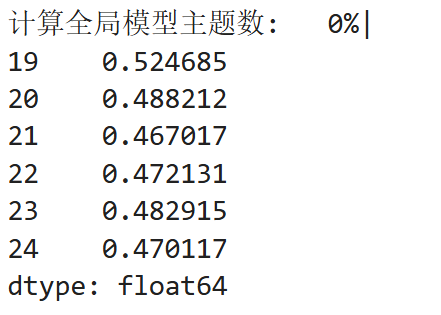
\includegraphics[width=0.5\textwidth]{Q2CV1} 
		\caption{\centering Coherence scores for topic numbers 19 to 24. The highest score is observed at 19 topics, suggesting it as the optimal choice for this model.}		
	\end{figure}
	
	We train the final LDA model (\texttt{lda\_model}) with 19 topics using optimized
	settings, evaluate the model with c\_v coherence score and save the model
	outputs, cleaned corpus, and topic descriptions for further analysis.
	\begin{python}
# Train the optimized final model with enhanced parameters for better convergence and topic separation
topics = 19

logging.basicConfig(level=logging.INFO, format='%(asctime)s - %(levelname)s - %(message)s')
# Optimized parameters for better convergence and topic distinction
lda_model = LdaMulticore(
    corpus=initial_dict["all_corpus"],
    id2word=initial_dict["overall_dict"],
    num_topics=topics,
    random_state=100,
    chunksize=100,           # Significantly reduced: increases update frequency and improves convergence
    passes=300,              # Moderately reduced: adjusted to work with other optimized parameters
    iterations=150,          # Newly added: increase iterations per pass
    alpha=0.01,              # Changed from 'asymmetric' to a small value: promotes document-topic sparsity and improves topic distinction
    eta=0.01,                # Changed from 'auto' to a small value: promotes word-topic sparsity and reduces topic mixing
    decay=0.5,               # Newly added: controls learning rate decay, improving convergence stability
    offset=1.0,              # Newly added: initial value for learning rate
    minimum_probability=0.01, # Newly added: filters out low-probability topic assignments
    per_word_topics=False,
    workers=None,            # Enables parallelization to speed up training
    eval_every=20            # Reduces evaluation frequency to lower computational cost
)
# Model evaluation
chmodel = CoherenceModel(
        model=lda_model,
        texts=initial_dict["all_original_text"],
        dictionary=initial_dict["overall_dict"],
        coherence="c_v"
    )
cv=chmodel.get_coherence()
cv
# Create unique directories for each LDA model
# That's because all variables are unique for each LDA model due to different stopword set
model_id=f"{topics}_{str(cv)[2:6]}"
# Model ID are designed as "[number of topics]_[CV score]", is unique for each model

path=f"output/lda_model/lda_{model_id}"
if not os.path.exists(path):
    os.makedirs(path)

path=f"output/lda_model/lda_{model_id}/cleaned_data"
if not os.path.exists(path):
    os.makedirs(path)

path=f"output/lda_model/lda_{model_id}/visualization"
if not os.path.exists(path):
    os.makedirs(path)

# Save LDA model
with open(f"output/lda_model/lda_{model_id}/lda_{model_id}.pkl",'wb') as f:
    pickle.dump(lda_model,f)

# Save cleaned data
with open(f"output/lda_model/lda_{model_id}/cleaned_data/cleaned_data.pkl", "wb") as f:
    pickle.dump(cleaned_data,f)

# Save original text
with open(f"output/lda_model/lda_{model_id}/all_original_text.pkl","wb") as f:
        pickle.dump(initial_dict["all_original_text"],f)
        
# Get all topics words and weights
all_topics_words = lda_model.show_topics(num_topics=-1, num_words=40, formatted=False)

markdown_content=f"## {topics} topics, cv={str(cv)[2:6]}\n\n"

for topic_id, topic_words_with_weights in all_topics_words:
        markdown_content += f"### Topic {topic_id}:\n" 
        
        
        for word, weight in topic_words_with_weights:
            markdown_content += f"- `{word}`: {weight:.4f}\n"
        markdown_content += "\n" 

# Save topic words and weights to markdown file
with open(f"output/lda_model/lda_{model_id}/lda_{model_id}.md", "w", encoding="utf-8") as f:
        f.write(markdown_content)
	\end{python}
	
	After examining the model outputs, we observed that some meaningless or
	unrepresentative words still remain in the model. This is primarily because
	the Twitter dataset contains a substantial amount of internet slang (e.g., "omg") that was not
	fully removed during the initial data cleaning process. To address this
	issue, we manually add these terms to the stopword list and re-run the LDA
	modeling process iteratively until we obtain a model with a high c\_v
	coherence score and minimal noise from irrelevant terms.
	
	The model we finally settled on is model \texttt{lda\_19\_5687}, with the highest high
	c\_v coherence score 0.5687. With this model, we will visualize the features
	of MBTI Twitter topics.
	
	
	\subsubsection{Result Visualization and Topic Evaluation}
	To start up the topic evaluation process, we need to import necessary
	libraries; define MBTI types,dimensions and groups; as well as load LDA
	model and cleaned data.
		\begin{python}
# Import necessary libraries
%matplotlib widget
import pyLDAvis
import pyLDAvis.gensim_models as gensimvis
import seaborn as sns
import matplotlib.pyplot as plt
from mpl_toolkits.mplot3d import Axes3D
import pandas as pd
import numpy as np
import pickle
from tqdm.auto import tqdm
import gensim.corpora as corpora
from gensim.models import LdaModel
from collections import defaultdict
from data_clean import Data_to_Clean,Data_to_Analyze
import warnings
warnings.filterwarnings('ignore')
from sklearn.cluster import KMeans
from sklearn.decomposition import PCA
from sklearn.preprocessing import StandardScaler

# Ensure the plots are displayed correctly
plt.rcParams['axes.unicode_minus']=False
sns.set_style("whitegrid")
sns.set_palette("husl")

# Define MBTI types
MBTI_types=[
    'istj','isfj','infj','intj',
    'istp','isfp','infp','intp',
    'estp','esfp','enfp','entp',
    'estj','esfj','enfj','entj'
]

# Define MBTI dimensions
mbti_dimensions={
    'E': ['estp','esfp','enfp','entp','estj','esfj','enfj','entj'],
    'I': ['istj','isfj','infj','intj','istp','isfp','infp','intp'],
    'S': ['istj','isfj','istp','isfp','estp','esfp','estj','esfj'],
    'N': ['infj','intj','infp','intp','enfp','entp','enfj','entj'],
    'T': ['intj','intp','entj','entp','istj','istp','estj','estp'],
    'F': ['isfj','infj','isfp','infp','esfj','enfj','esfp','enfp'],
    'J': ['istj','isfj','infj','intj','estj','esfj','enfj','entj'],
    'P': ['istp','isfp','infp','intp','estp','esfp','enfp','entp']
}

# Define MBTI groups
mbti_groups={
    "analysts":["intj","intp","entj","entp"],
    "diplomats":["infj","infp","enfj","enfp"],
    "sentinels":["istj","isfj","istp","isfp"],
    "explorers":["isfp","istp","estp","esfp"]
}

# Load LDA model and data
# Model ID are designed as "[number of topics]_[CV score]",is unique for each model


def load_lda_data():
    # Load LDA model
    lda_model=pickle.load(open(f"output/lda_model/lda_{model_id}/lda_{model_id}.pkl","rb"))
    print(f"Successfully loaded LDA model with {lda_model.num_topics} topics")
    
    # Load original text data
    all_original_text=pickle.load(open(f"output/lda_model/lda_{model_id}/all_original_text.pkl","rb"))
    print(f"Successfully loaded original text data with {len(all_original_text)} documents")
    
    return lda_model,all_original_text
    

# Load cleaned data grouped by MBTI types
def load_mbti_data():
    file_path=f"output/lda_model/lda_{model_id}/cleaned_data/cleaned_data.pkl"
    with open(file_path,'rb') as f:
        cleaned_data=pickle.load(f)
    print(f"Cleaned data loaded successfully")

    return cleaned_data

# Execute file loading
lda_model,all_original_text=load_lda_data()
mbti_cleaned_data=load_mbti_data()
		\end{python}
	
	To better interpret topics and detect patterns in the data, we construct a
	class \texttt{LDATopicAnalyzer}, which integrates the LDA model with the
	MBTI-annotated dataset. This class performs several key functions: 
	\begin{enumerate}
		\item Transforms input texts into bag-of-words representations, computes
		topic distributions for each document, and groups these distributions by
		MBTI type to observe group-level thematic tendencies.
		\item Supports generating interactive visualizations through pyLDAvis, which
		is created and saved to html.
		\item Provides tools to extract representative keywords per topic and
		optionally identify and exclude noise topics that carry little interpretive
		value. 
	\end{enumerate}
	  
	\begin{python}
# Create a class for LDA visualization
class LDATopicAnalyzer:
    def __init__(self,lda_model,texts,mbti_data):
        self.model=lda_model
        self.texts=texts
        self.mbti_data=mbti_data
        self.dictionary=lda_model.id2word
        self.corpus=[self.dictionary.doc2bow(text) for text in texts]
        self.noise_topic=[]
        self.topic_distributions=None
        self.mbti_topic_distributions=None
        
    def create_pyldavis_visualization(self,save_path=f"final_output/lda_visualization.html"):
        
        print("Creating pyLDAvis visualization...")
        # Prepare pyLDAvis visualization
        vis_data=gensimvis.prepare(
            self.model,
            self.corpus,
            self.dictionary,
            sort_topics=False
        )
        
        # Save as HTML file
        pyLDAvis.save_html(vis_data,save_path)
        print(f"pyLDAvis visualization saved to: {save_path}")
        
        # Display in notebook
        pyLDAvis.enable_notebook()
        return pyLDAvis.display(vis_data)
    
    def get_topic_distributions(self):
        """Get topic distributions for documents"""
        print("Calculating topic distributions...")
        
        topic_distributions=[]
        for doc_bow in tqdm(self.corpus,desc="Calculating topic distributions"):
            doc_topics=self.model.get_document_topics(doc_bow,minimum_probability=0)
            topic_probs=[prob for _,prob in doc_topics]
            topic_distributions.append(topic_probs)
        
        self.topic_distributions=np.array(topic_distributions)
        return self.topic_distributions
    
    def calculate_mbti_topic_distributions(self):
        """Calculate topic distributions for each MBTI type"""
        print("Calculating topic distributions for each MBTI type...")
        
        mbti_topic_dist={}
        
        for mbti_type in MBTI_types:
            if mbti_type in self.mbti_data and len(self.mbti_data[mbti_type].data) > 0:
                # Create corpus for documents of this MBTI type
                mbti_corpus=[self.dictionary.doc2bow(doc) for doc in self.mbti_data[mbti_type].data["posts"]]
                
                # Calculate topic distributions
                topic_sums=np.zeros(self.model.num_topics)
                doc_count=0
                
                for doc_bow in mbti_corpus:
                    doc_topics=self.model.get_document_topics(doc_bow,minimum_probability=0)
                    for topic_id,prob in doc_topics:
                        topic_sums[topic_id]+=prob
                    doc_count+=1
                
                # Calculate average topic distributions
                if doc_count>0:
                    mbti_topic_dist[mbti_type]=topic_sums/doc_count
                else:
                    mbti_topic_dist[mbti_type]=np.zeros(self.model.num_topics)
            else:
                mbti_topic_dist[mbti_type]=np.zeros(self.model.num_topics)
        
        self.mbti_topic_distributions=mbti_topic_dist
        return mbti_topic_dist
    
    def get_topic_words(self,num_words=10):
        """Get keywords for each topic"""
        topic_words={}

        for topic_id in range(self.model.num_topics):
            words=self.model.show_topic(topic_id,topn=num_words)
            topic_words[topic_id]=[word for word,_ in words]
        return topic_words
    
    def add_noise_topics(self,*topic_ids):
        """Define noise topics"""
        for i in topic_ids:
            self.noise_topic.append(i)
# Create analyzer instance

analyzer=LDATopicAnalyzer(lda_model,all_original_text,mbti_cleaned_data)
print("LDA topic analyzer created successfully!")

# Create pyLDAvis interactive visualization
vis=analyzer.create_pyldavis_visualization()
vis
	\end{python}

	The interactive topic visualization generated by pyLDAvis can be accessed at
	the following link:
	\url{https://dominicmin.github.io/Intro_to_DS_Assignment/lda_visualization.html}.
	\cref{fig:HTML} shows the initial state of the HTML file: 
	
		\begin{figure}[H]
			\centering
			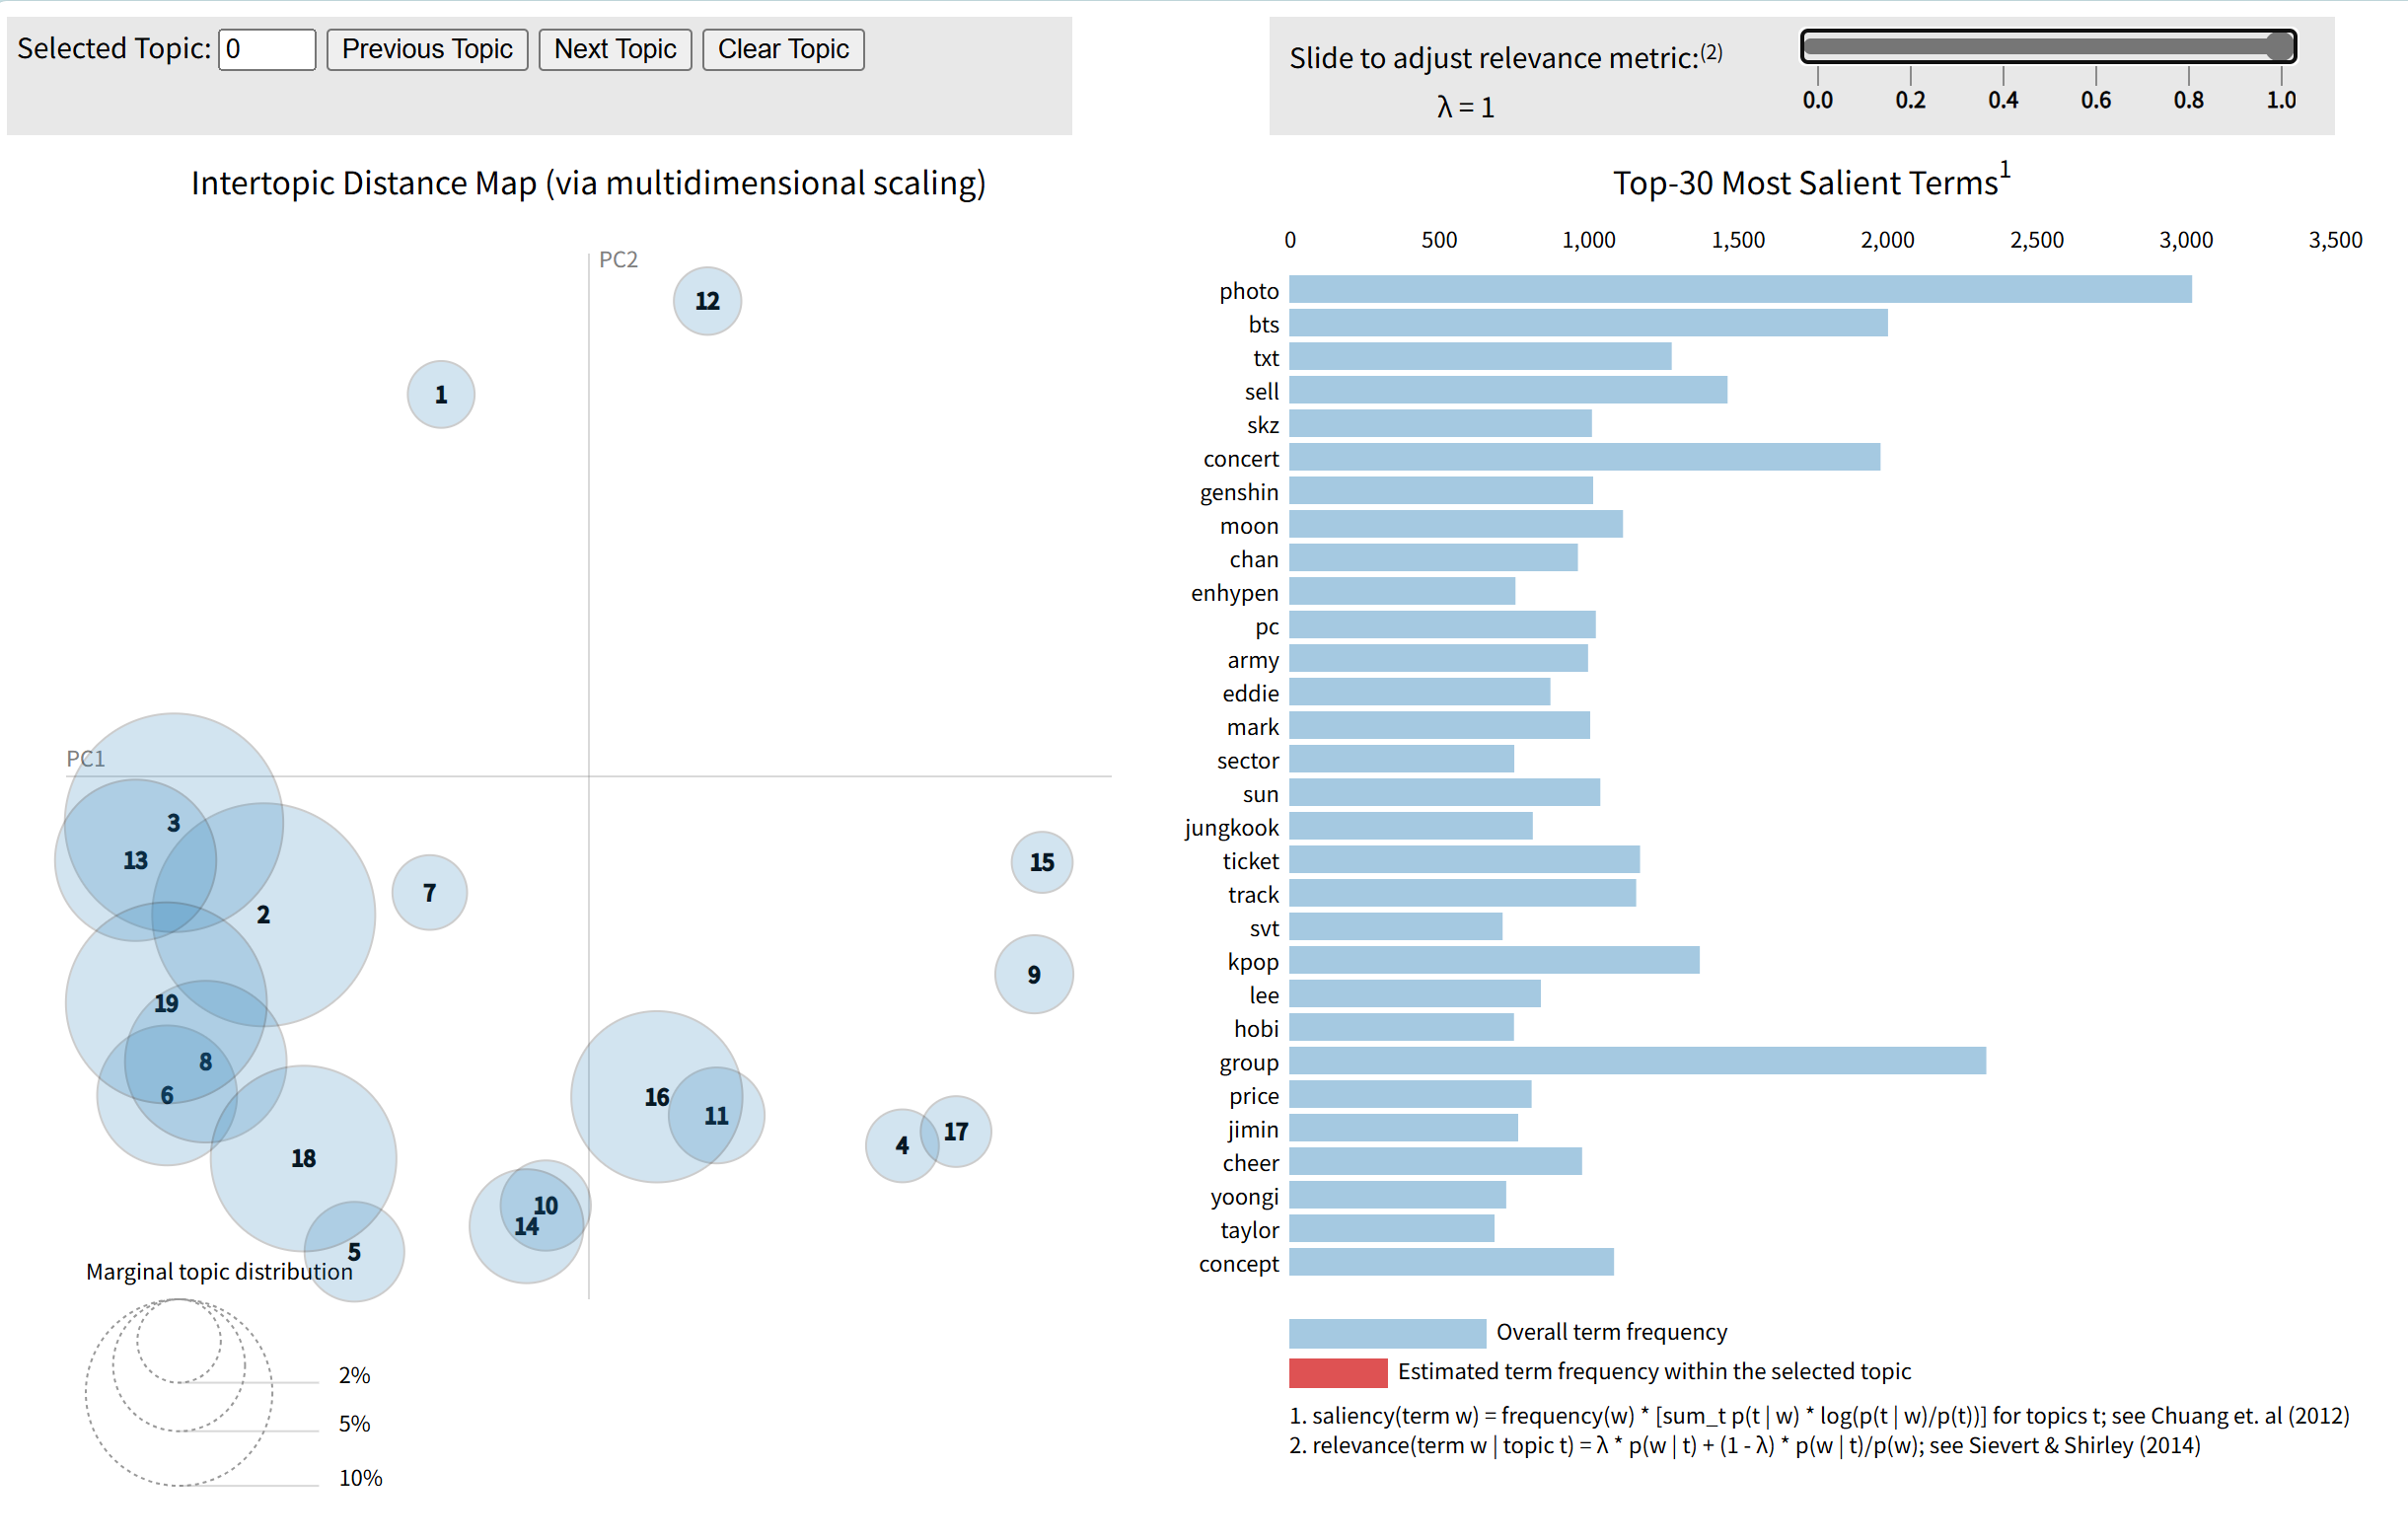
\includegraphics[width=1\textwidth]{Q2html0} 
			\caption{\centering Screenshot of the initial state of the HTML file}	
			\label{fig:HTML}	
			\vspace{-0.5em} % 稍微向上调整,减少与标题的间距
    \parbox{\linewidth}{\small \textbf{Note:} The topic indices in the HTML file
	are offset by +1 compared to the LDA model output (i.e., Topic 1 in HTML is
	Topic 0 in LDA).}
		\end{figure}
	
	
	As shown in \cref{fig:HTML}, on the left side of the HTML file, the
	\textbf{Intertopic Distance Map} visualizes the relationships between topics
	in two dimensions. A possible interpretation is that each bubble represents
	a distinct topic, with its area indicating the proportion of tokens (words)
	in the entire corpus attributed to that topic. Larger bubbles correspond to
	topics that account for a greater share of the corpus. The position and
	overlapping of each bubble reflects semantic similarity—the farther apart
	two bubbles are and the less the bubbles overlap, the less semantically %e can explain 2 and 3 pc projection
	related the corresponding topics. However, as will be demonstrated later,
	this interpretation fails to accurately characterize certain topics.
	
	On the right side of the HTML page, the adjustable relevance metric of the
	selected topic is presented alongside the Top-30 Most Salient Terms. For
	each term, its overall frequency in the corpus is displayed as a blue
	histogram, while its estimated frequency within the selected topic is shown
	in red. Users can adjust the value of $\lambda$ to observe changes in term
	saliency and the relationship between a term’s overall frequency and its
	topic-specific relevance. 
	
	When $\lambda$ is slided to the position 0, the terms that are unique in
	this topic are prior exhibited. These words are characterized by high
	distinctiveness, meaning they appear much more frequently in the selected
	topic compared to their frequency across the entire corpus. As a result,
	they serve as strong discriminators, helping to differentiate this topic
	from others. Although such terms may not be the most frequent within the
	topic itself, they often carry greater semantic specificity and are
	particularly useful for interpreting nuanced or domain-specific themes.
	However, because this setting emphasizes uniqueness over prevalence, it may
	occasionally highlight low-frequency or noisy terms, which should be
	interpreted with caution in topic labeling.
	
	Meanwhile, when $\lambda$ is slided to the position 1, these words represent
	the most commonly occurring terms in the topic and therefore reflect its
	core semantic content. This setting is particularly useful for understanding
	the dominant themes or main discourse of the topic. However, because it does
	not account for how exclusive a term is to the topic, some high-frequency
	terms that are also common in other topics may be included, potentially
	reducing the distinctiveness of the topic’s representation.
	 
	From \cref{fig:HTML}, we can gain an overview of our modeling outcome.
	Topic 18 has the largest bubble, indicating that it is the most prevalent
	topic in the corpus. Topics 9, 15, 4, and 17 are located farther away from
	the other topics, suggesting a clear semantic distinction. In contrast,
	Topics 3, 13, 2, 8, 6, 19, and 18 exhibit notable spatial overlap,
	indicating only minor differences in their semantic content. In the whole
	corpus, the most reoccurring words are mostly related to the entertainment
	fandom and game fandom.
	%e 并不完全表示,没什么特点,联系岔开
	
	By selecting different topics and adjusting the value of $\lambda$, we can
	summarize the central theme of each topic, determine whether it is a noise
	topic, and assess its degree of semantic coherence.
	
	Take topic 12 as an example, when $\lambda$ is set to 0, the most relevant
	terms—such as trump, biden, republican, democrat, congress, and abortion—are
	highly distinctive and strongly associated with U.S. political discourse.
	These terms are not only topically specific but also exclusive to this
	topic, suggesting a focused and meaningful theme centered around American
	politics, government institutions, and social issues.	In contrast, when
	$\lambda$ is increased to 1, the top terms—such as state, country, child,
	gun, and law—shift toward higher-frequency words within the topic. Although
	some of these terms are more general, they still retain political relevance
	and semantic consistency with the topic’s core, indicating that the theme is
	robust across different relevance metrics. In conclusion, the presence of
	consistently interpretable and contextually appropriate terms at both
	extremes of the $\lambda$ scale demonstrates that topic 13 exhibits a
	relatively high degree of semantic coherence. The lack of function words,
	formatting artifacts, or off-topic vocabulary suggests that this is not a
	noise topic, but rather a well-defined and meaningful cluster within the
	corpus.
	\begin{figure}[H]
			\centering
			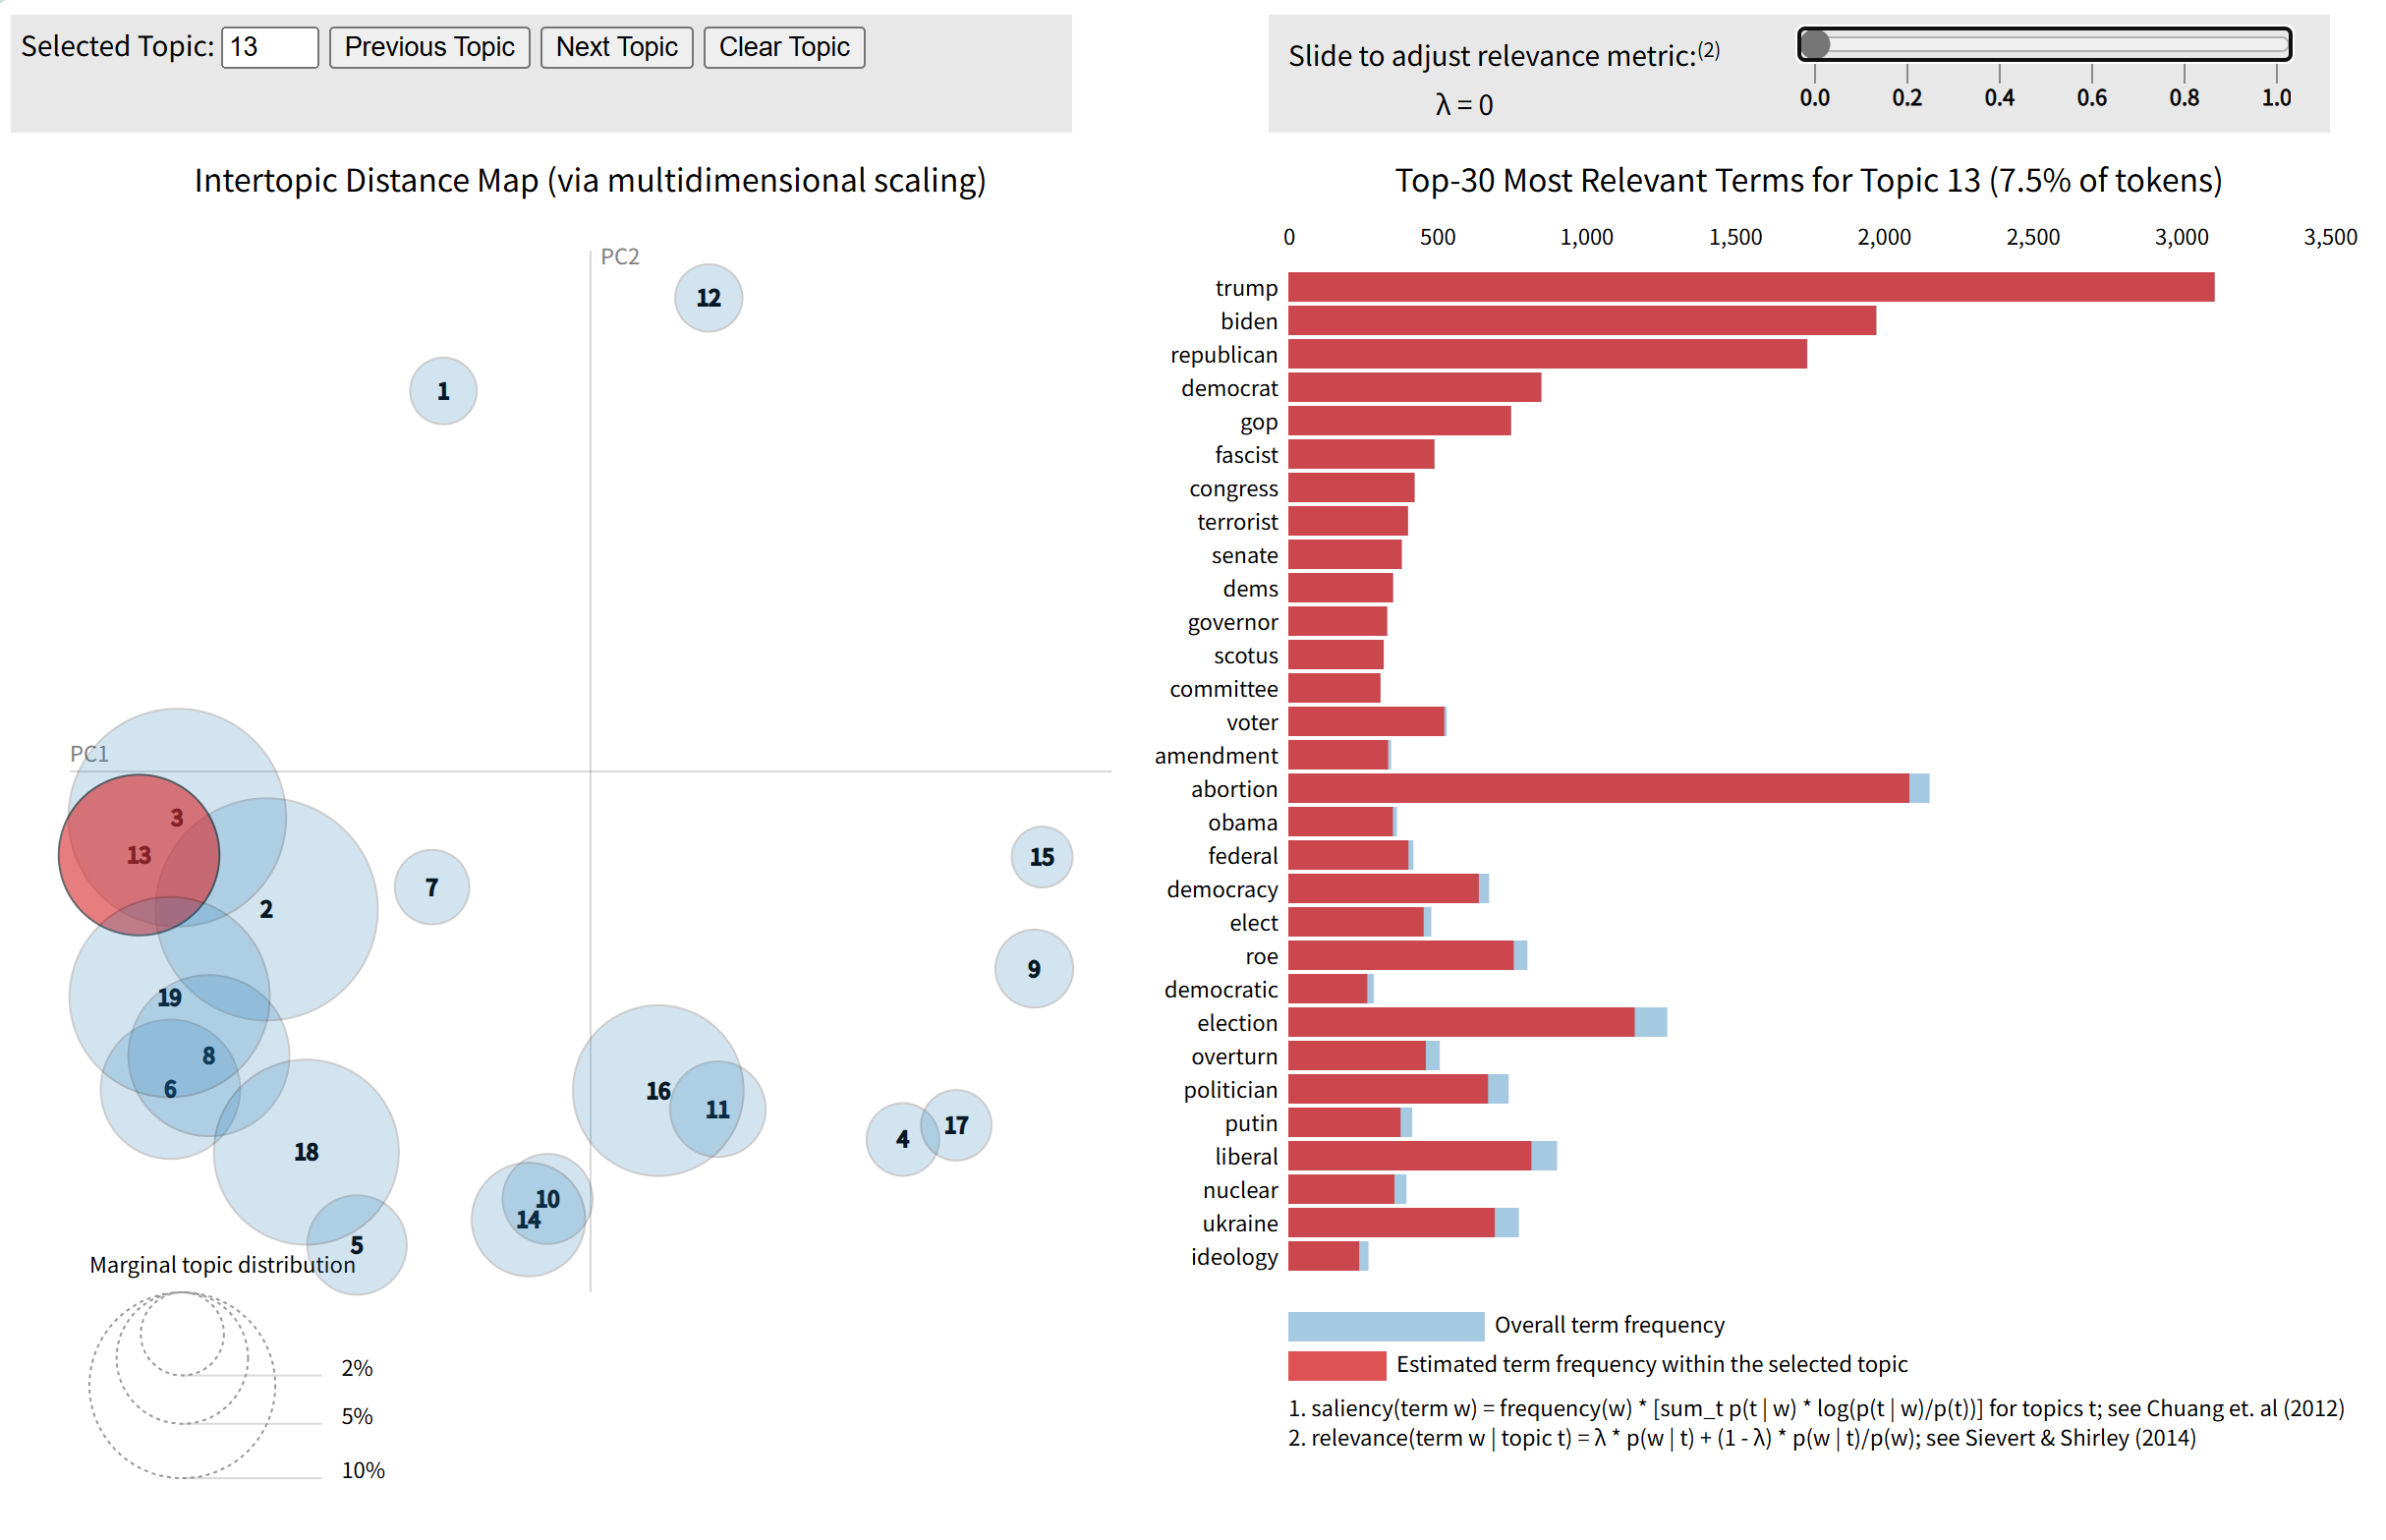
\includegraphics[width=0.9\textwidth]{Q2r0} 
			\caption{\centering HTML page with Topic 12 selected and $\lambda$=0}		
	\end{figure}
	\begin{figure}[H]
			\centering
			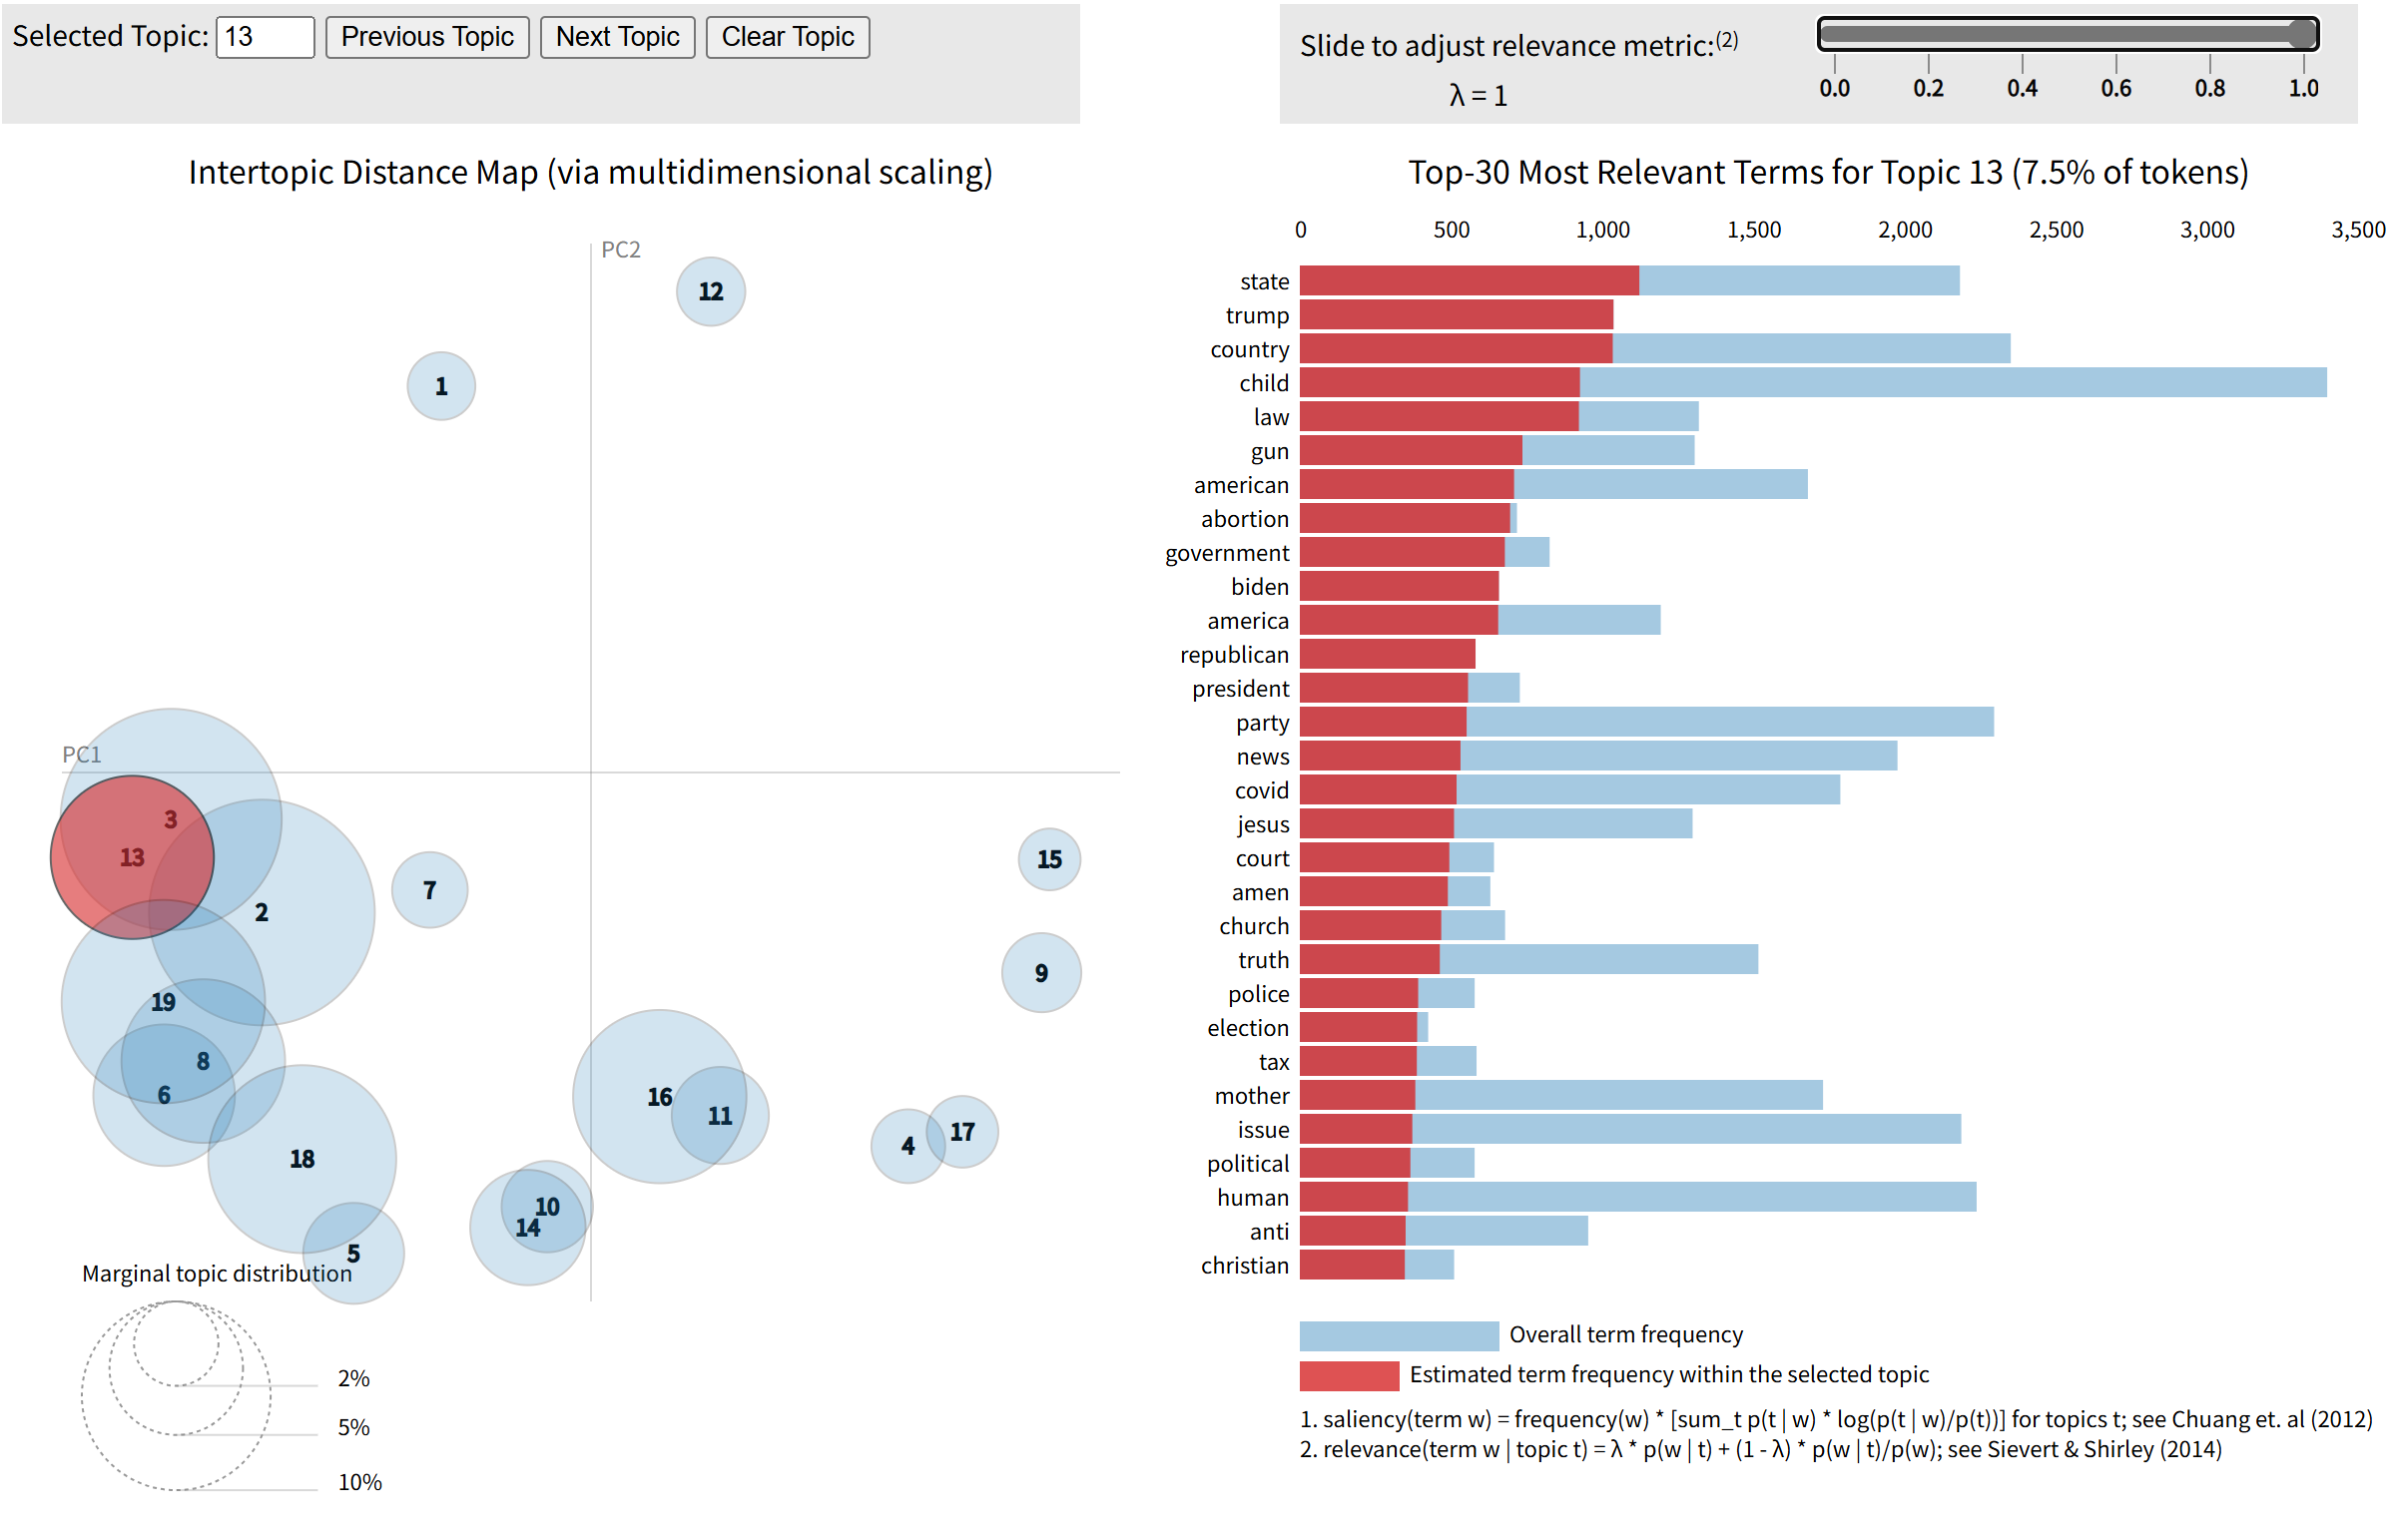
\includegraphics[width=0.9\textwidth]{Q2r1} 
			\caption{\centering HTML page with Topic 12 selected and $\lambda$=0}		
	\end{figure}
	By applying this method to all the topics, we can conclude the following
	topic modeling result:
	\begin{itemize}
	\item High semantic coherence - 8 topics:
	
		Topic 0: Astrology/Zodiac
		
		Topic 3: K-pop Groups (TXT/NCT)
		
		Topic 4: Western TV Shows (Stranger Things/Heartstopper)
		
		Topic 6: Gaming (Genshin Impact)
		
		Topic 8: K-pop Groups (SEVENTEEN/ATEEZ)
		
		Topic 9: Western Pop Music/Celebrities
		
		Topic 10: K-pop Group (BTS)
		
		Topic 14: K-pop Group (ENHYPEN)
		
		Topic 16: K-pop Group (Stray Kids)
	\item 	Medium semantic coherence - 6 topics:
	
		Topic 2: Academic/Business/Personal Development
		
		Topic 5: Gender Identity/LGBTQ+/Mental Health
		
		Topic 7: Food/Weight Management/Eating Disorders
		
		Topic 11: Merchandise Trading/Collectibles
		
		Topic 12: Politics/Social Issues
		
		Topic 17: Anime/Manga/Fan Culture
		
		Topic 1: Daily Life and traveling
	\item 	Low semantic coherence - 1 topic:
	
		Topic 15: K-pop Industry General
	\item Noise Topics - 2 topics:
	
		Topic 13: Mixed Social Media Expressions
		
		Topic 18: Generic Terms/Mixed Content
	\end{itemize}
	
	Interestingly, when linking the interpreted topics to their corresponding
	bubbles, we observe that although Topic 2 (Academic/Business/Personal
	Development) and Topic 12 (Politics/Social Issues) show considerable overlap
	in the Intertopic Distance Map, they are not semantically similar. This
	mismatch occurs because high-dimensional topic data is projected onto a
	two-dimensional space.
	%e can explain in detail 
	%需要写噪音去除
	%The noise topics Topic 13 and Topic 18 should be excluded in further analysis and clustering. However, due to the limitation of our dataset, if we exclude such a big topic as Topic 18, 
	
	\subsubsection{Topic Distribution}
	We begin by calculating and visualizing topic distribution.
	\begin{python}
# Calculate topic distributions for MBTI types

mbti_topic_dist=analyzer.calculate_mbti_topic_distributions()
topic_words=analyzer.get_topic_words()

# Create topic distribution DataFrame
topic_dist_df=pd.DataFrame(mbti_topic_dist).T
topic_dist_df.columns=[f"Topic {i}" for i in range(len(topic_dist_df.columns))]
topic_dist_df.drop([f"Topic {i}" for i in analyzer.noise_topic],
                   axis=1,
                   inplace=True)

print("MBTI type topic distribution calculation completed!")
print(f"Topic distribution matrix shape: {topic_dist_df.shape}")

# Display first few rows
print("\nPreview of topic distributions for each MBTI type:")
display(topic_dist_df.head())
	\end{python}
	\begin{figure}[H]
		\centering
		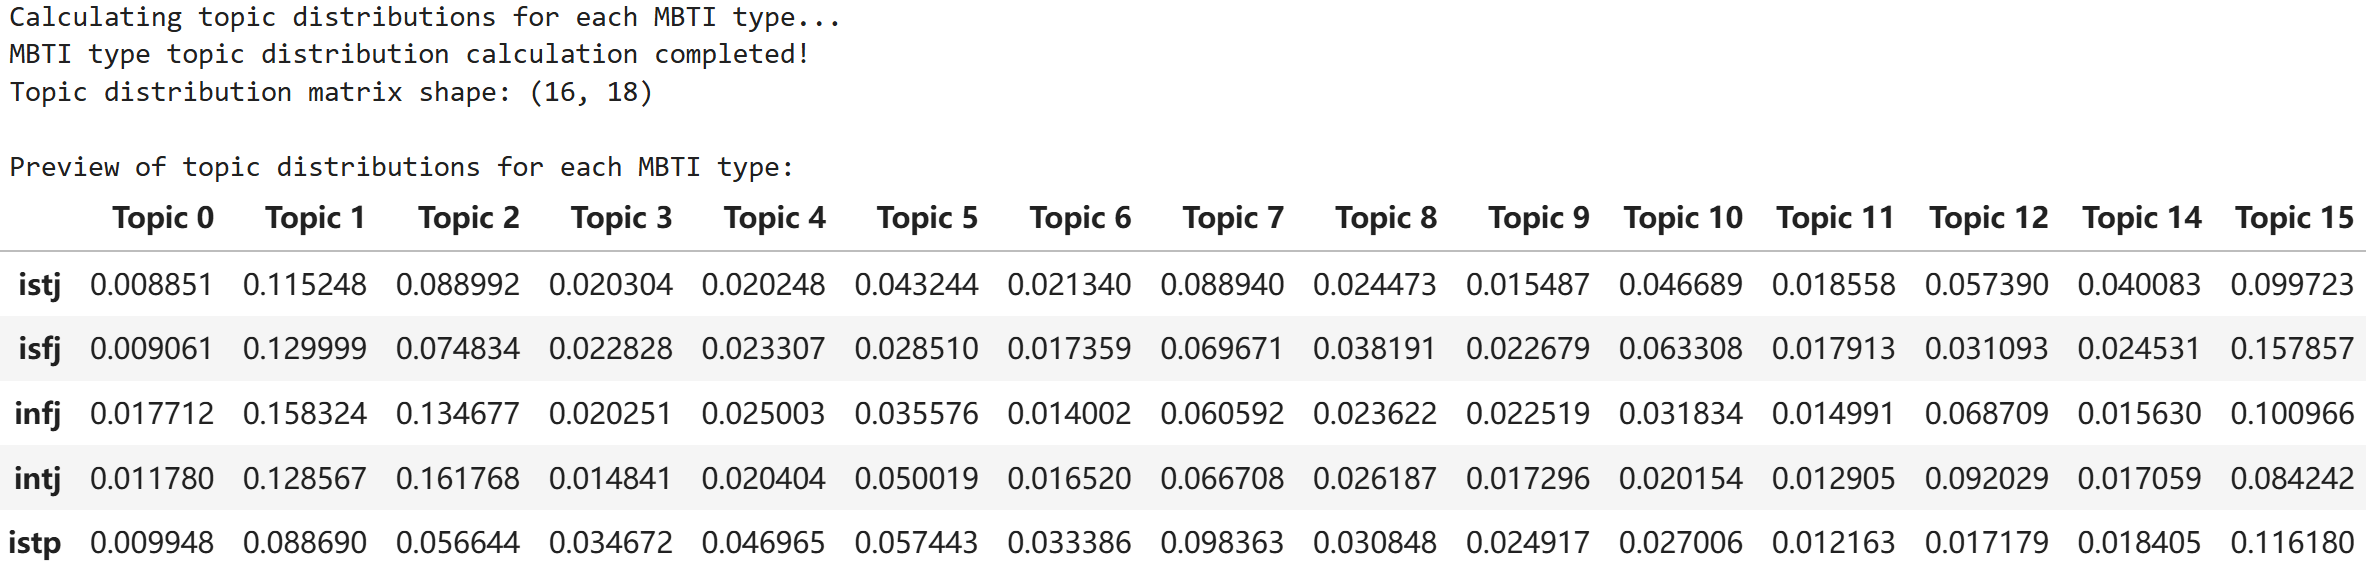
\includegraphics[width=1\textwidth]{Q2row} 
		\caption{\centering Preview of first few rows}		
	\end{figure}
	
	A heatmap is generated based on the computed values to visually represent the results.
	\begin{figure}[H]
		\centering
		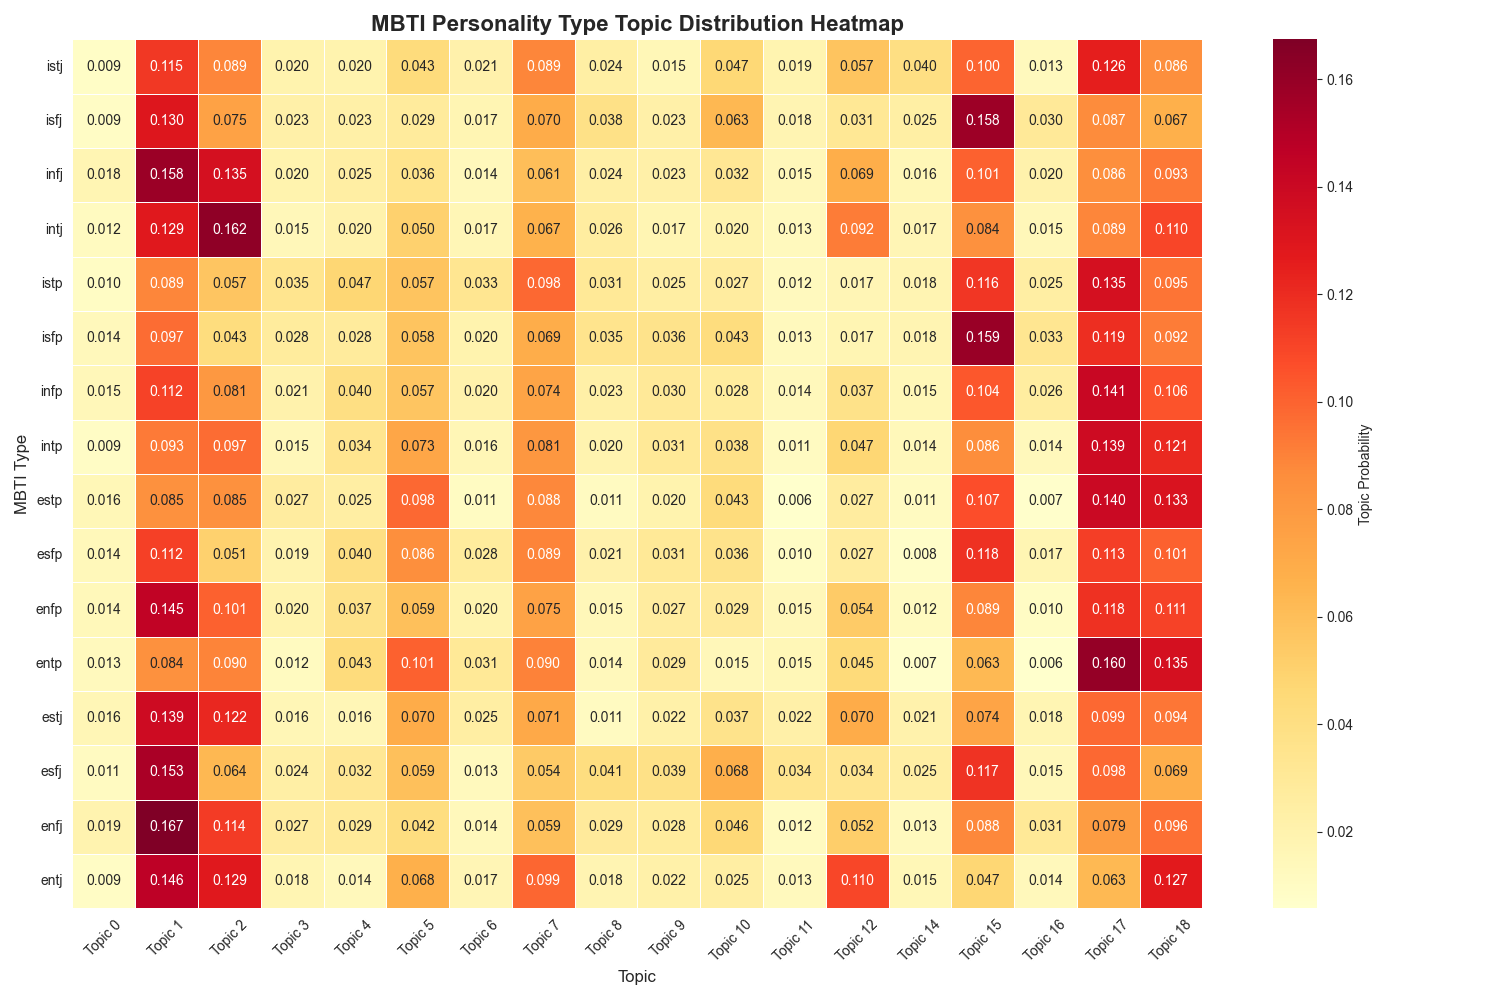
\includegraphics[width=1\textwidth]{Q2hmap} 	
	\end{figure}
	
	The heatmap provides an intuitive visual indication of topic popularity.
	Specifically, Topics 1 (Daily Life and traveling),
	2 (Academic/Business/Personal Development), 15 (K-pop Industry General), and
	17 (Anime/Manga/Fan Culture) exhibit darker red shades, suggesting they are
	more frequently discussed. A more rigorous, quantitative analysis of topic
	popularity will be presented further on.
	
	To assist with our interpretation with the heatmap, we calculate the overall
	popularity of each topic.
	\begin{python}
# Create topic keyword cloud summary
def create_topic_wordcloud_summary(topic_words,topic_dist_df):
    """Create topic keyword summary"""
    print("=" * 60)
    print("Topic keyword summary")
    print("=" * 60)
    
    # Calculate overall popularity of each topic
    topic_popularity=topic_dist_df.mean().sort_values(ascending=False)
    
    for i,(topic_idx,popularity) in enumerate(topic_popularity.items()):
        topic_num=int(topic_idx.replace('Topic',''))
        print(f"\nTopic {topic_num} (Popularity: {popularity:.3f}):")
        print(f"Keywords: {','.join(topic_words[topic_num][:8])}")
        
        # Find the MBTI type that most prefers this topic
        topic_col=f"Topic {topic_num}"
        if topic_col in topic_dist_df.columns:
            top_mbti=topic_dist_df[topic_col].nlargest(3)
            print(f"Most preferred MBTI types: {','.join([f'{mbti}({score:.3f})' for mbti,score in top_mbti.items()])}")
        
        if i >= 9:  # Only show top 10 topics
            break


create_topic_wordcloud_summary(topic_words,topic_dist_df)
	\end{python}
	%e better change source figure
	 This gives us the following summary:
	 \begin{figure}[H]
	 		\centering
	 		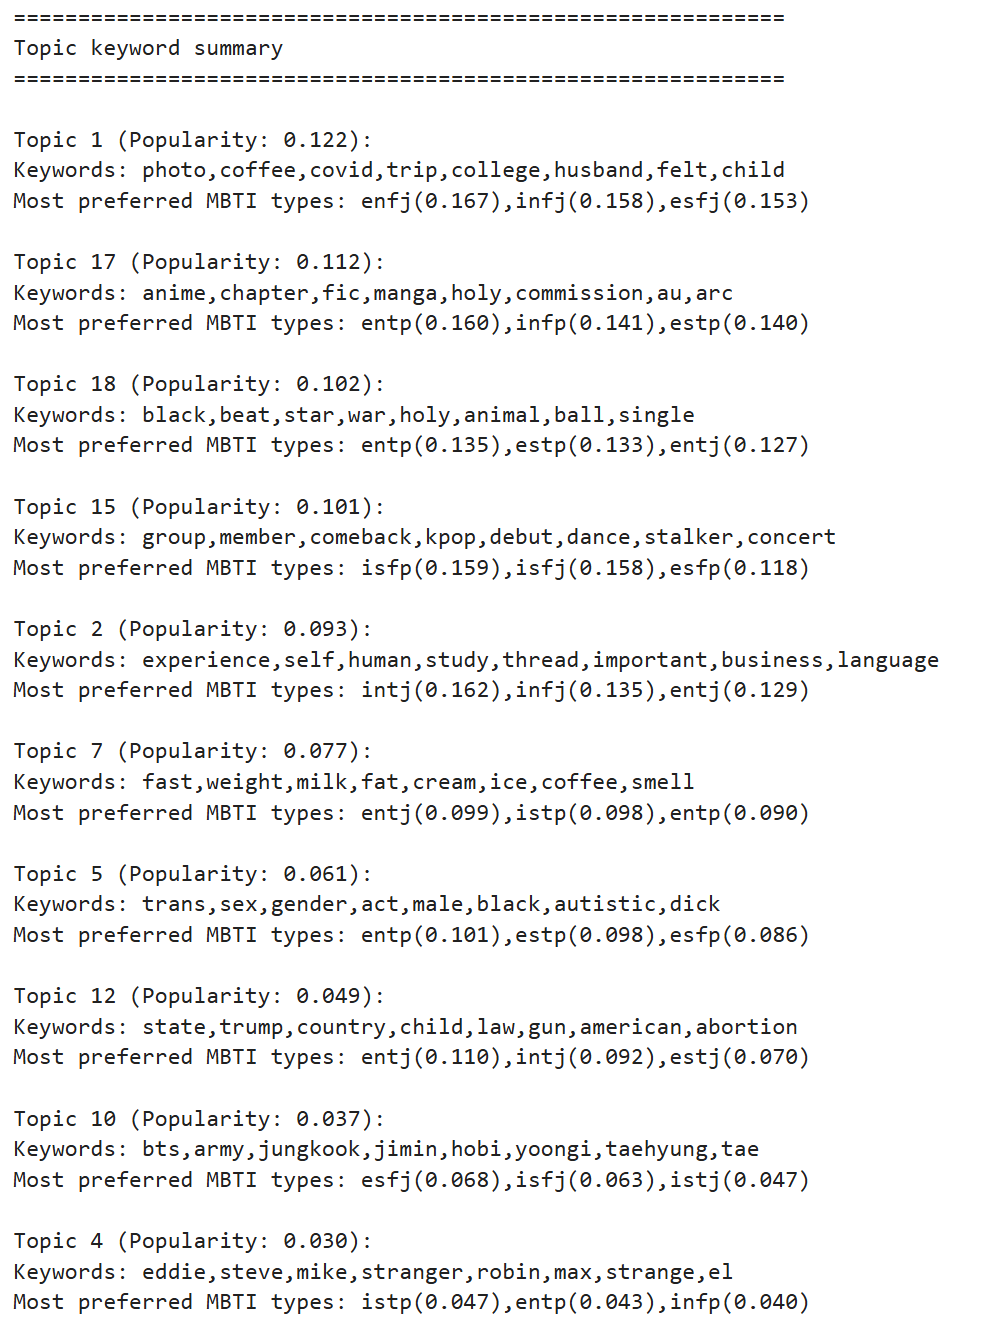
\includegraphics[width=0.5\textwidth]{Q2topsum} 	
	 \end{figure}
	 
	 With the aid of the summary statistics, we can find distinct MBTI
	 engagement patterns across different semantic domains:
	\begin{itemize}
	\item Topic 15 (K-pop fandom activities): characterized by group debuts,
	comebacks, and concerts; demonstrates strong engagement among ISFP, ISFJ,
	and ESFP types, underscoring the intersection of sensory enjoyment and
	emotional engagement.
	\item Topic 14 (lightweight, emotionally-driven daily expression): resonates
	with SP types who prioritize spontaneity and immediate experiential sharing.
	\item Topic 7 (sensory experiences related to food and comfort): emphasizes
	fast food, coffee, and cream, aligning with ISTP and ESTP preferences for
	direct sensory satisfaction.
	\item Topic 17 (strategic, abstract, and fandom-oriented discussions):
	involves anime, manga, and fan fiction; attracts ENTP, INFP, and ESTP types,
	indicating alignment with analytical and imaginative discourse.
	\item Topic 2 (experiential and intellectual reflections): appeals to INTJ,
	ENTJ, and INFJ types, reflecting their preference for profound, thoughtful,
	and self-reflective content.
	\item Topic 18 (adventurous and competitive themes): includes sports and
	competitions; engages ENTP, ESTP, and ENTJ personalities drawn to intense
	experiences.
	\item Topic 5 (identity and socially charged discussions): covers gender,
	sexuality, and societal roles; garners interest from ENTP, ESTP, and ESFP
	types open to explorative and provocative topics.
	\item Topic 12 (politically charged discourse): focuses on societal debates
	like Trump, guns, and abortion; attracts ENTJ, INTJ, and ESTJ types inclined
	toward policy and governance.
	\item Topic 10 (BTS fandom): features BTS member names; resonates with ESFJ
	and ISFJ types, highlighting community-oriented engagement.
	\item Topic 4 (Stranger Things franchise): references characters like Eddie
	and Steve; shows engagement from ISTP, ENTP, and INFP types, indicating
	analytical and introspective affinities.
	\end{itemize}
	
	Having observed engagement patterns of individual MBTI types, we compare the
	topic preference patterns of different MBTI groups.
	\begin{python}
# Create MBTI dimension topic preference analysis
def analyze_mbti_dimensions(topic_dist_df,mbti_dimensions=mbti_dimensions):
    """Analyze topic preferences for MBTI four dimensions"""
    dimension_analysis={}
    
    for dim,types in mbti_dimensions.items():
        # Calculate average topic distribution for this dimension type
        dim_types_in_data=[t for t in types if t in topic_dist_df.index] # t is a single type
        dimension_analysis[dim]=topic_dist_df.loc[dim_types_in_data].mean() # mean of the topic distribution for this dimension/group type
    
    return pd.DataFrame(dimension_analysis)

dimension_pairs=[('E','I'),('S','N'),('T','F'),('J','P')]
pair_names=['Extrovert vs Introvert','Sense vs Intuition','Thinking vs Feeling','Judging vs Perceiving']
    

def create_dimension_comparison(dimension_df,file_name,dimension_pairs=dimension_pairs,pair_names=pair_names,comment=None):
    """Create MBTI dimension topic preference comparison chart"""
    fig,axes=plt.subplots(int(len(dimension_pairs)/2),2,figsize=(16,6*int(len(dimension_pairs)/2)))
    axes=axes.flatten()
        
    for i,((dim1,dim2),pair_name) in enumerate(zip(dimension_pairs,pair_names)):
        if dim1 in dimension_df.columns and dim2 in dimension_df.columns:
            # Calculate difference
            diff=dimension_df[dim1]-dimension_df[dim2]
            
            # Create bar chart
            x_pos=range(len(diff))
            colors=['red' if x < 0 else 'blue' for x in diff]
            
            axes[i].bar(x_pos,diff,color=colors,alpha=0.7)
            axes[i].axhline(y=diff.apply(abs).quantile(q=0.85),color='red',linestyle='--',alpha=0.3,label='85% Quantile Line')
            axes[i].axhline(y=-diff.apply(abs).quantile(q=0.85),color='red',linestyle='--',alpha=0.3)
            axes[i].axhline(y=0,color='black',linestyle='-',alpha=0.3)
            axes[i].set_title(f'{pair_name} Diff in Topic Preference',fontsize=12,fontweight='bold')
            axes[i].set_xlabel('Topic')
            axes[i].set_ylabel(f'{dim1} - {dim2} Preference Difference')
            axes[i].set_xticks(x_pos)
            axes[i].set_xticklabels([j for j in list(topic_dist_df.columns)],rotation=45)
            axes[i].grid(True,alpha=0.3)
            axes[i].legend()
    fig.suptitle("MBTI Group Topic Preference Comparison",fontsize=16,fontweight='bold',y=1)
    plt.tight_layout()
    plt.figtext(0.5, 0.02,comment,ha='center',fontsize=10)
    plt.savefig(f'output/lda_model/lda_{model_id}/visualization/{file_name}.png',dpi=300,bbox_inches='tight')
    plt.savefig(f'final_output/{file_name}_drop13_18.png',dpi=300,bbox_inches='tight')
    plt.show()


dimension_df=analyze_mbti_dimensions(topic_dist_df)
print("MBTI dimension topic preference analysis:")
display(dimension_df.head())

# create_dimension_comparison(dimension_df,"mbti_dimension_comparison")
group_pairs=[
            ('analysts','diplomats'),
            ('sentinels','explorers'),
            ('sentinels','diplomats'),
            ('explorers','diplomats'),
            ('sentinels','analysts'),
            ('explorers','analysts')
             ]
group_names=['Analysts vs Diplomats',
             'Sentinels vs Explorers',
             'Sentinels vs Diplomats',
             'Explorers vs Diplomats',
             'Sentinels vs Analysts',
             'Explorers vs Analysts'
             ]

group_df=analyze_mbti_dimensions(topic_dist_df,mbti_groups)
create_dimension_comparison(group_df,"mbti_group_comparison",group_pairs,group_names)
	\end{python}
	\begin{figure}[H]
			\centering
			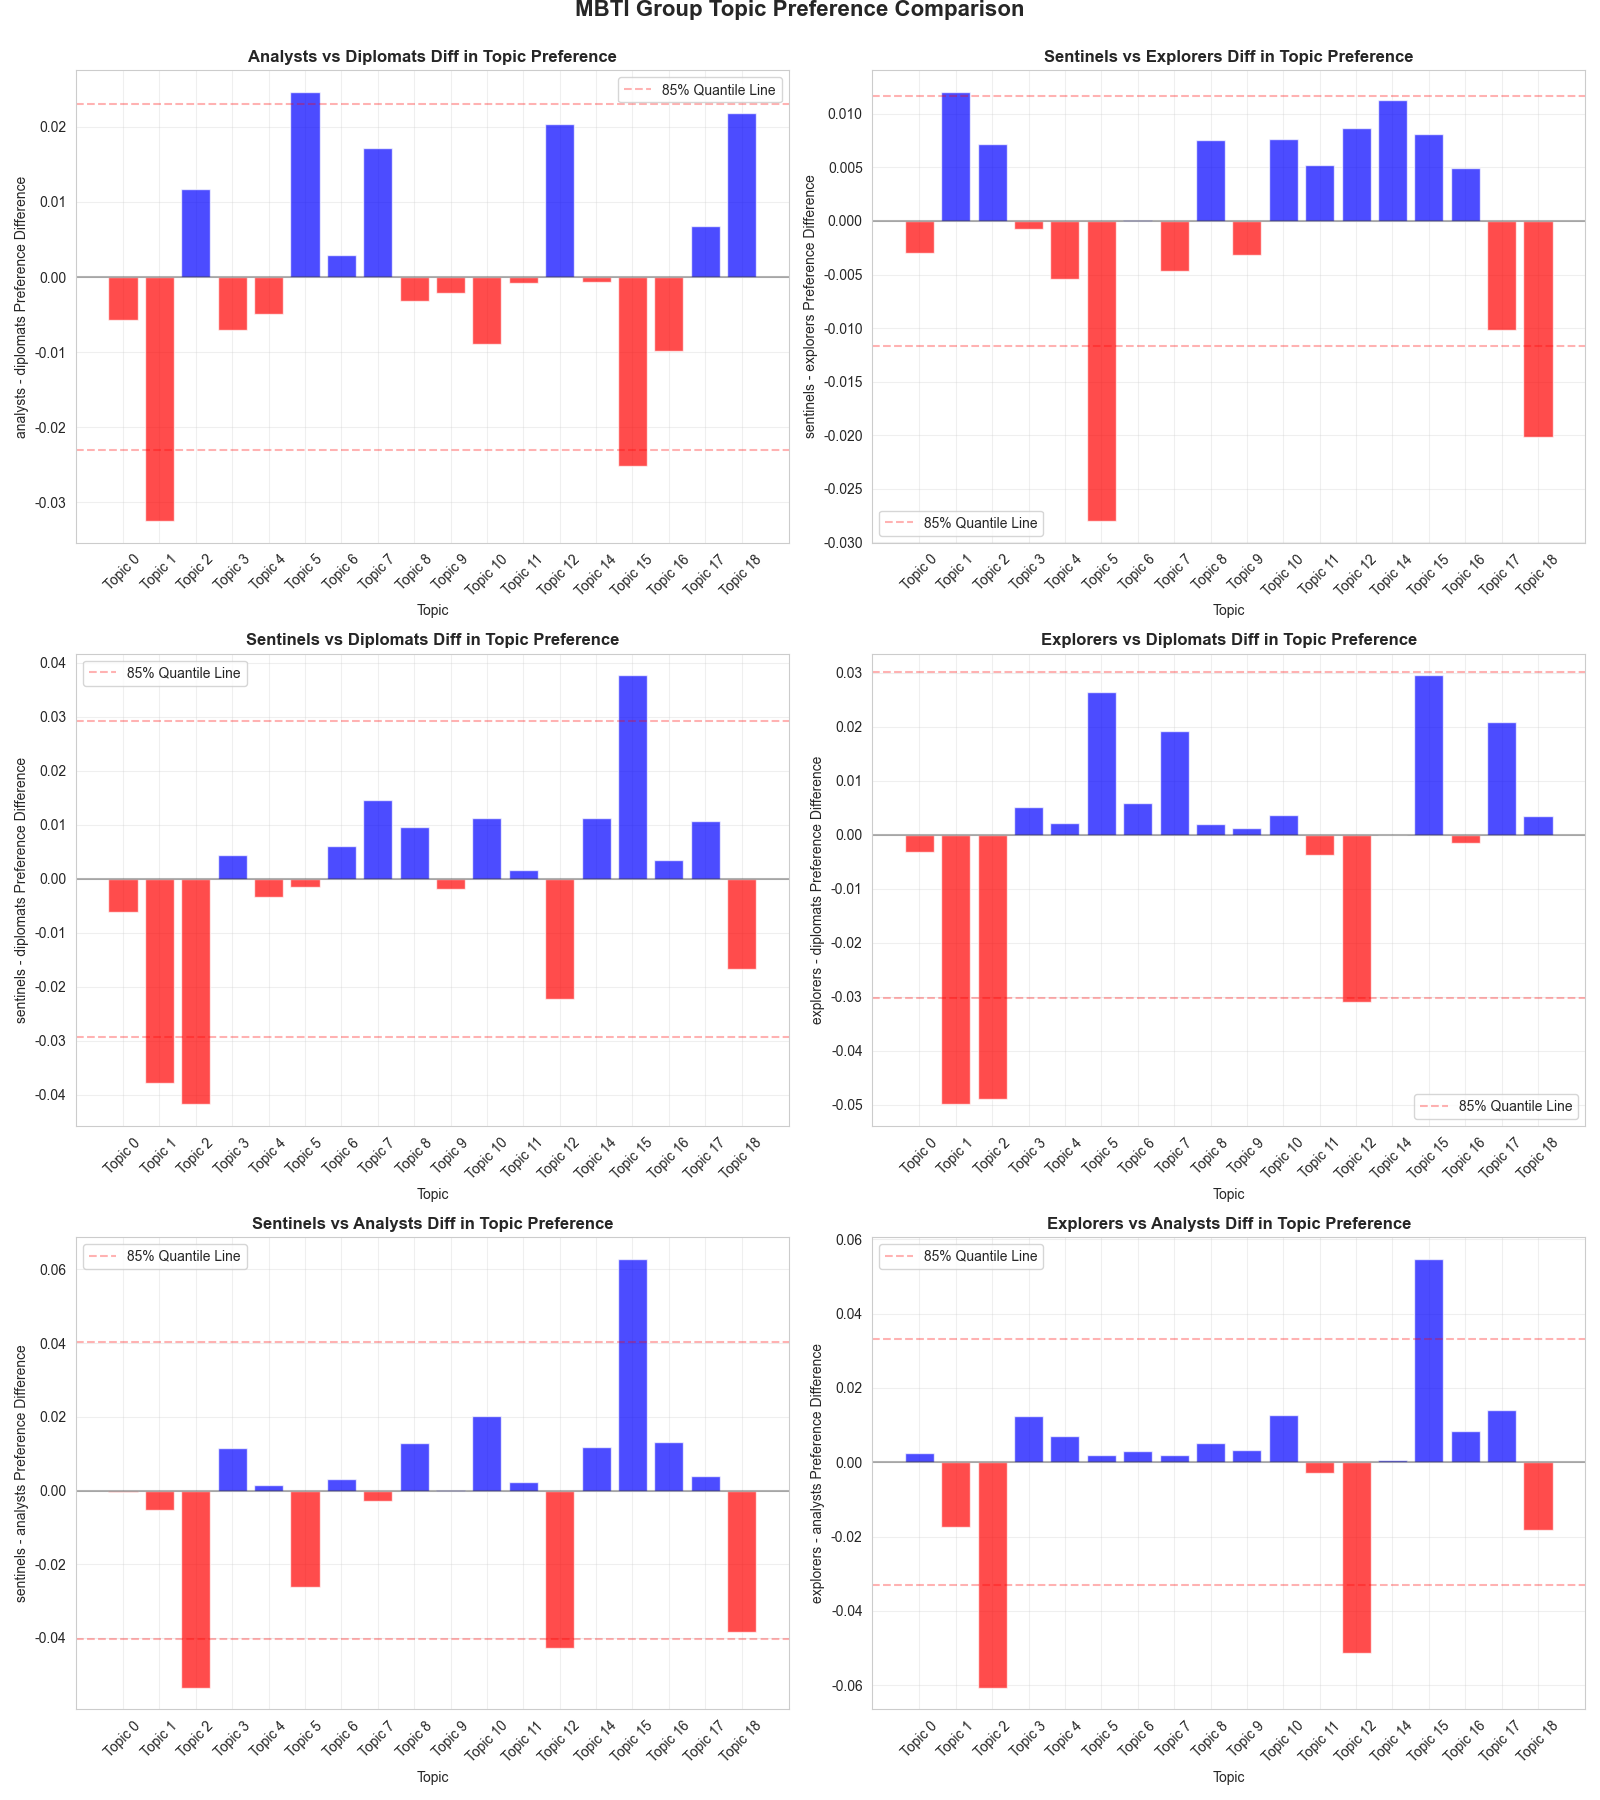
\includegraphics[width=1\textwidth]{Q2grouppre} 	
	\end{figure}
	
	%e better change source of figure
	%e dimentional analysis missing
	For a unified comparison, we set the standard of significantly different as
	any absolute topic-preference gap that surpasses the 85th-percentile
	threshold, which is indicated by the red dashed line in each subplot.
	
	From these 6 comparisons we can come up with the following conclusions:
	\begin{enumerate}
	\item Analysts show a clear surplus of discussion in the “Gender /
	Mental-Health” and “Politics / Social Issues” topics, whereas Diplomats
	contribute markedly less to these threads. This suggests that the NT
	temperaments are more inclined toward idea-driven or policy-oriented
	debates, while the NF group devotes its energy to lighter, experience-based
	conversations such as travel logs and casual fandom chatter.
	\item When Sentinels are compared with Explorers, the former post more
	frequently about day-to-day planning, travel itineraries, and the buying or
	trading of collectibles. Explorers, in contrast, engage less with these
	logistics-heavy themes and more with personal identity talk. This difference
	implies that SJ personalities favour order and tangible exchanges, while SP
	personalities gravitate toward spontaneous self-expression.
	\item Sentinels dominate K-pop industry news and merchandise exchange, yet
	they underperform on topics related to academic or personal growth.
	Therefore, the data indicate a Sentinel preference for operational or
	execution-oriented content, whereas Diplomats continue to focus on
	introspection and self-development narratives.
	\item Explorers outpace Diplomats in discussions about ENHYPEN fandom, the
	game Genshin Impact, and LGBTQ identity issues, but fall behind in travel
	diaries, study tips, and political conversations. This result reinforces the
	notion that SP types pursue sensory entertainment and identity exploration,
	whereas NF types lean toward reflective or civic-minded themes.
	\item Sentinels tweet far more about mainstream idols such as ENHYPEN and
	BTS, while Analysts turn their attention to academically oriented or
	self-improvement threads. We conclude that SJ users are deeply involved in
	collective fan activities, whereas NT users remain focused on knowledge and
	analytical depth.
	\item Explorers lead Analysts in anime and manga chatter, yet they post
	significantly less about academic and political issues. The evidence points
	to an SP preference for leisure-centred pop-culture content, contrasting
	with an NT preference for intellectually demanding discussions.
	\end{enumerate}
	

	
	%Analyzing from the perspective of MBTI functional groups, clearer behavioral and cognitive preferences emerge.
	
	%对四个维度的称呼不统一,需调查专业写法
	%\begin{itemize}
	%\item NF types(Diplomats) consistently gravitate toward emotionally and symbolically rich discussions (Topics 1, 2), emphasizing their values-driven communication style and expressive tendencies. 
	%\item SP(Explorers) types distinctly favor immediate experiential and sensory-focused topics (Topics 7, 14, 15), indicative of their present-oriented, sensory-driven inclinations. 
	%\item NT(Analysts) types predominantly engage in abstract reasoning, strategic analyses, and fandom discussions that encourage complex intellectual engagement (Topics 2, 5, 17).
	%\item SJ(Sentinels) types display balanced interests, engaging prominently with mainstream cultural phenomena and structured, community-centric discussions (Topics 1, 10, 17), reflecting their preference for structured interaction, practical feasibility, and communal harmony.
	%\end{itemize}
	
 	\subsubsection{MBTI type Clustering} 
	%e change logic
	Using LDA modeling, we have identified the topic preference different of
	MBTI personality types. To which extent does the estimated or stereotyped
	topic preference of the official MBTI groups align with their realistic
	behaviors? We cluster MBTI types to find out.
	
	Reducing high-dimensional topic distributions into a three-dimensional
	principal component space is necessary for K-means clustering to be
	preformed. So, PCA dimensionality reduction is preformed before we preform
	K-means clustering
	\begin{python}
def create_mbti_clustering_analysis_3d(n_clusters,topic_dist_df=topic_dist_df):
    
    # Standardize data
    scaler=StandardScaler()
    scaled_data=scaler.fit_transform(topic_dist_df)
    
    # 3D PCA dimensionality reduction
    pca=PCA(n_components=3)
    pca_3d_data=pca.fit_transform(scaled_data)
    
    # K-means clustering (on 3D data)
    kmeans=KMeans(n_clusters=n_clusters, random_state=42)
    clusters=kmeans.fit_predict(pca_3d_data)  # Note: clustering on 3D data
	\end{python}

	After clustering, we print PCA variance to see if PCA dimensionality
	reduction is effective.
	\begin{python}
# Print variance explained
print(f"3D PCA variance explained:")
print(f"PC1: {pca.explained_variance_ratio_[0]:.3f}")
print(f"PC2: {pca.explained_variance_ratio_[1]:.3f}")  
print(f"PC3: {pca.explained_variance_ratio_[2]:.3f}")
print(f"Total: {pca.explained_variance_ratio_.sum():.3f}")
	\end{python}
	
	The results are:
	
	\texttt{PC1: 0.328}
	
	\texttt{PC2: 0.265}
	
	\texttt{PC3: 0.117}
	
	\texttt{Total: 0.709}
	
	With a total of 70.9\% of information successfully reserved, our
	dimensionality reduction is successful.
	
	To interpret our clustering results, it is necessary for us to find out what
	PC1, PC2, PC3 represents respectively. So we print out the main contributing
	features of the three dimensions respectively and plot out PCA feature
	weights.
	\begin{figure}[H]
		\centering
		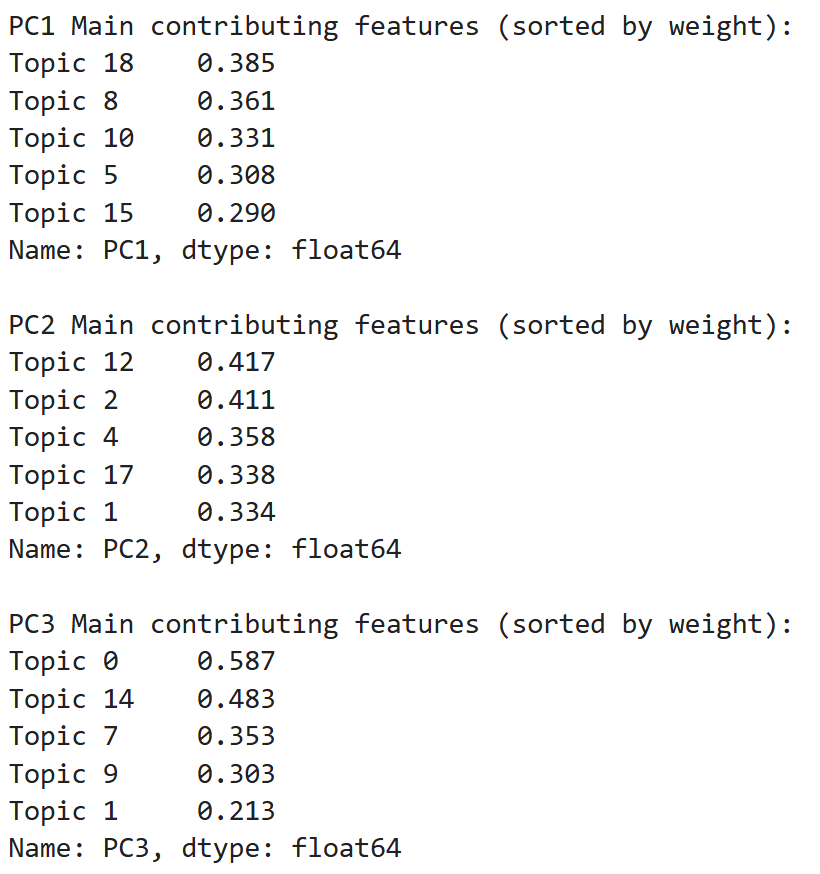
\includegraphics[width=0.5\textwidth]{Q2PCA1} 
		\caption{\centering Printed Main contributing features}		
	\end{figure}	
	\begin{figure}[H]
			\centering
			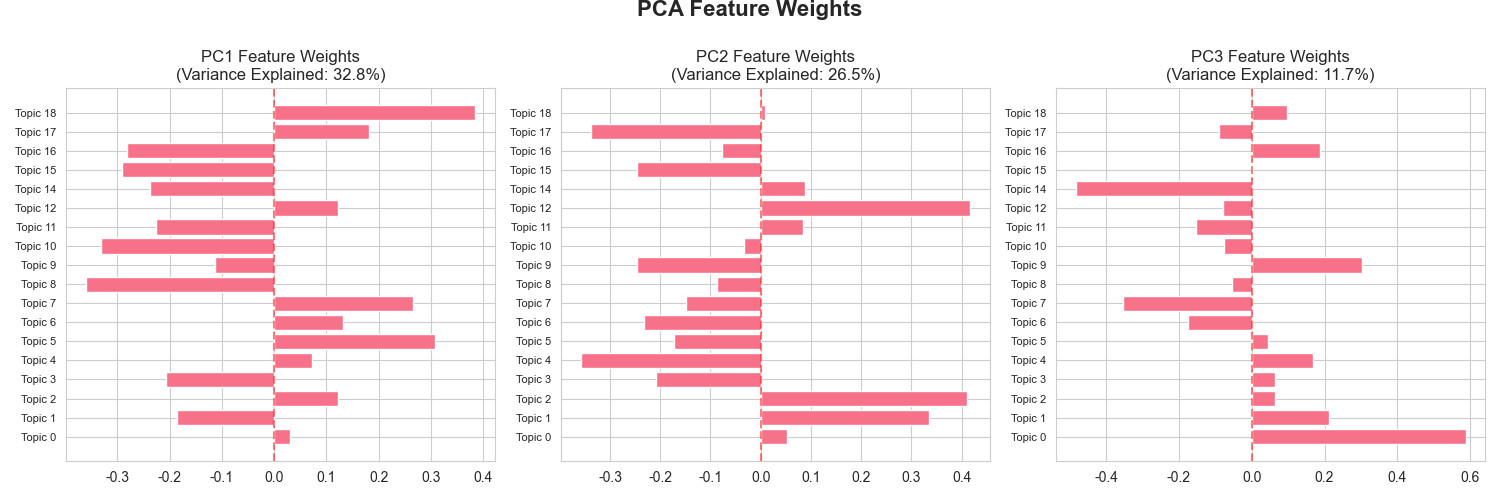
\includegraphics[width=1\textwidth]{Q2PCA2} 		
	\end{figure}
	
	By analyzing the printed features and plotted results, we approximately
	conclude the meaning of each axis:
	\begin{enumerate}
	\item PC1: Leisure \& Fandom vs. Everyday-life.
	\item PC2: Politics–Rationality vs. Entertainment–Support.
	\item PC3: Fragmented expressions vs. centralized fandom behavior
	\end{enumerate}
	
	6 distinctive clusters can be distinguished from our clustering results.
	\begin{python}
    # Print clustering results
    print("\nClustering results:")
    print("=" * 50)
    for cluster_id in range(n_clusters):
        # Get mbti types in the current cluster
        mbti_in_cluster=[topic_dist_df.index[i] for i in range(len(clusters)) if clusters[i] == cluster_id]
        # Convert to uppercase and sort
        mbti_in_cluster_upper=sorted([mbti.upper() for mbti in mbti_in_cluster])
        print(f"Cluster {cluster_id + 1}: {', '.join(mbti_in_cluster_upper)}")
    print("=" * 50)
	\end{python}

	\begin{figure}[H]
			\centering
			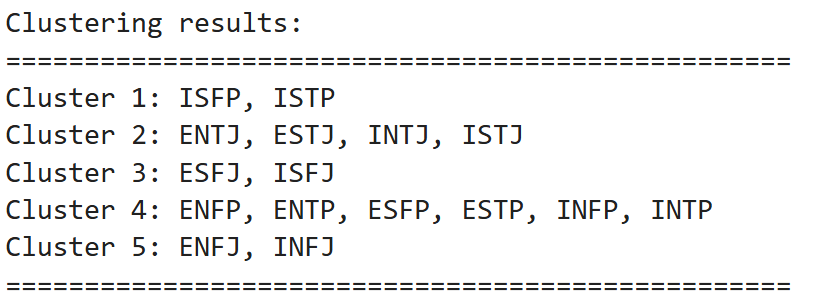
\includegraphics[width=0.5\textwidth]{Q2cluster1} 
			\caption{\centering Printed clustering results}		
	\end{figure}
	
	A 3-D scatter plot and it's 2-dimensional projection is plotted to visualize the results.
	\begin{python}
    # 3D visualization
    fig=plt.figure(figsize=(12, 9))
    ax=fig.add_subplot(111, projection='3d')
    
    # 3D scatter plot
    scatter=ax.scatter(pca_3d_data[:,0], pca_3d_data[:,1], pca_3d_data[:,2], 
                        c=clusters, cmap='viridis', s=100, alpha=0.7)
    
    # Add MBTI labels
    for i, mbti_type in enumerate(topic_dist_df.index):
        ax.text(pca_3d_data[i,0], pca_3d_data[i,1], pca_3d_data[i,2], 
               mbti_type.upper(), fontsize=10, fontweight='bold')
    
    ax.set_xlabel(f'PC1 ({pca.explained_variance_ratio_[0]:.1%} variance)')
    ax.set_ylabel(f'PC2 ({pca.explained_variance_ratio_[1]:.1%} variance)')
    ax.set_zlabel(f'PC3 ({pca.explained_variance_ratio_[2]:.1%} variance)')
    
    ax.set_title('3D MBTI Clustering Analysis Based on Topic Distribution', 
                fontsize=14, fontweight='bold')
    
    
    
    plt.colorbar(scatter)
    plt.show()
    
    
    return pca_3d_data, clusters
    fig, axes = plt.subplots(1, 3, figsize=(15, 5))
    axes[0].scatter(cl_analysis[0][:,0], cl_analysis[0][:,1], 
                            c=cl_analysis[1], cmap='viridis', s=100, alpha=0.7)
    axes[1].scatter(cl_analysis[0][:,0], cl_analysis[0][:,2], 
                            c=cl_analysis[1], cmap='viridis', s=100, alpha=0.7)
    axes[2].scatter(cl_analysis[0][:,1], cl_analysis[0][:,2], 
                            c=cl_analysis[1], cmap='viridis', s=100, alpha=0.7)
    axes[0].set_xlabel("PC1")
    axes[0].set_ylabel("PC2")
    axes[0].set_title("Projection of MBTI Types onto PC1 and PC2")
    axes[1].set_xlabel("PC1")
    axes[1].set_ylabel("PC3")
    axes[1].set_title("Projection of MBTI Types onto PC1 and PC3")
    axes[2].set_xlabel("PC2")
    axes[2].set_ylabel("PC3")
    axes[2].set_title("Projection of MBTI Types onto PC2 and PC3")
    for i, mbti_type in enumerate(topic_dist_df.index):
        axes[0].text(cl_analysis[0][i,0], cl_analysis[0][i,1], 
                   mbti_type.upper(), fontsize=10, fontweight='bold')
        axes[1].text(cl_analysis[0][i,0], cl_analysis[0][i,2], 
                   mbti_type.upper(), fontsize=10, fontweight='bold')
        axes[2].text(cl_analysis[0][i,1], cl_analysis[0][i,2], 
                   mbti_type.upper(), fontsize=10, fontweight='bold')
    fig.suptitle("Projection of MBTI Types onto PC1, PC2, and PC3", fontsize=14, fontweight='bold')
    plt.tight_layout()
    plt.savefig(f"output/lda_model/lda_{model_id}/visualization/mbti_clustering_projection.png")
    plt.savefig(f"final_output/mbti_clustering_projection.png")
    plt.show()
	\end{python}
	
	\begin{figure}[H]
			\centering
			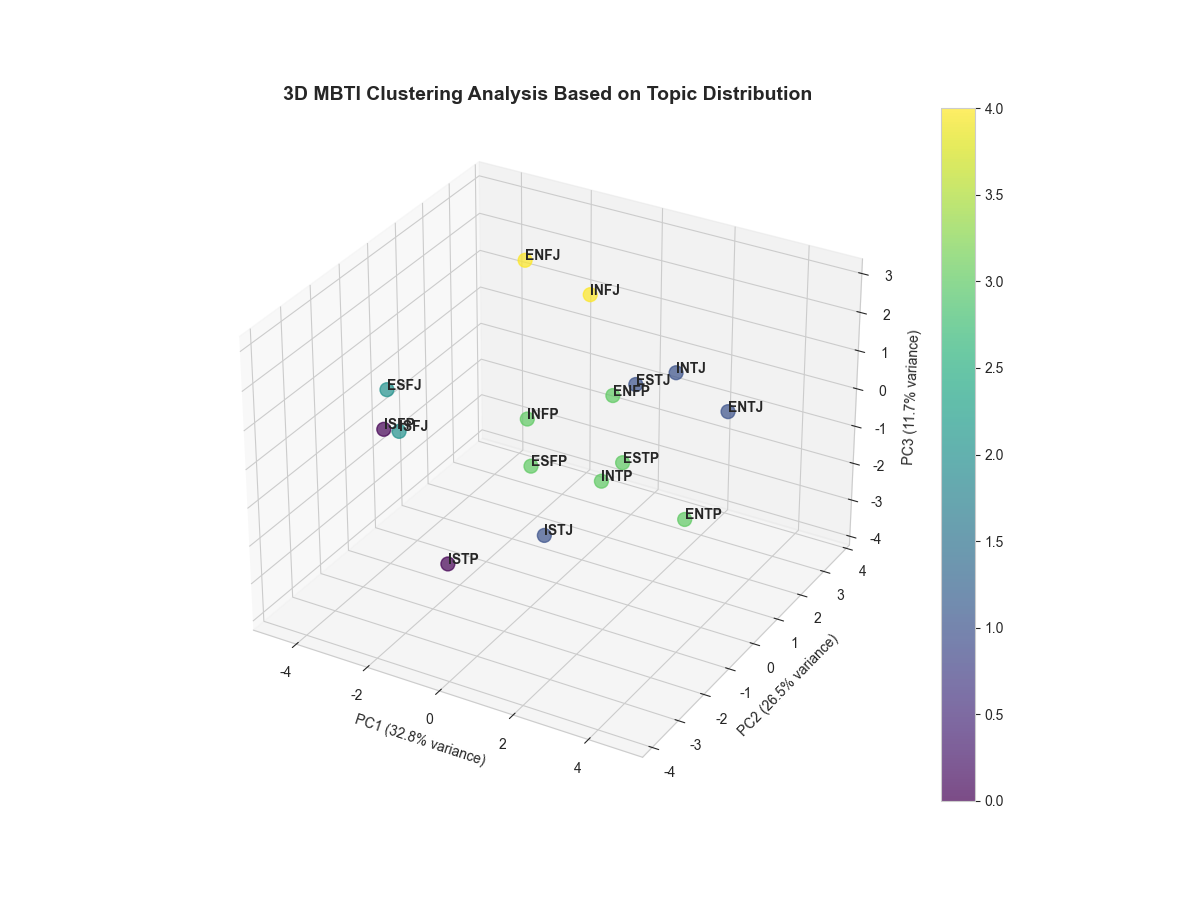
\includegraphics[width=0.9\textwidth]{Q23D} 	
	\end{figure}
	\begin{figure}[H]
			\centering
			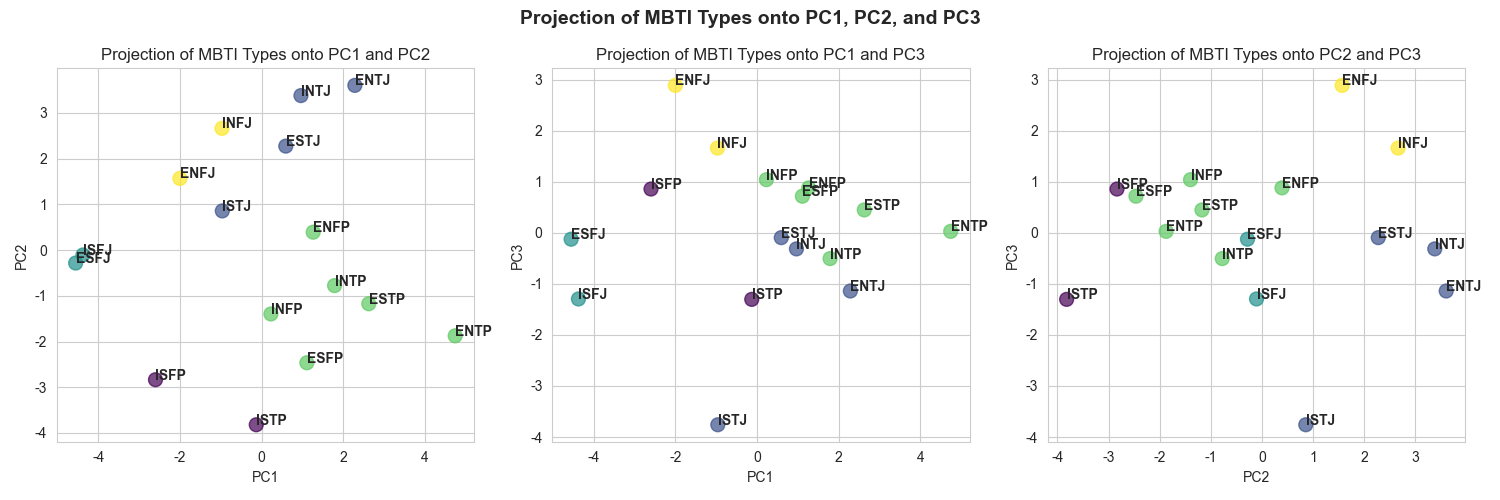
\includegraphics[width=0.9\textwidth]{Q22D} 	
	\end{figure}
	
	Using the concluded meaning of each axis, we can come up with the following conclusions:
	\begin{itemize}
	\item Cluster 1: ISFP, ISTP — leisure-oriented, low political talk,
	fragmented style
	\item Cluster 2: ENTJ, ESTJ, INTJ, ISTJ — everyday \& rational topics,
	highly centralised
	\item Cluster 3: ESFJ, ISFJ — life-focused, cooperative support behaviour
	\item Cluster 4: ENFP, ENTP, ESFP, ESTP, INFP, INTP — strong entertainment
	preference, fragmented expression
	\item Cluster 5: ENFJ, INFJ — politics / affect-driven, centralised fandom
	\end{itemize}
	
	This outcome aligns closely to the four MBTI groups, suggesting certain
	reliability of MBTI grouping.
	
	\subsection{Expressive Patterns of MBTI Personalities}
	\subsubsection{Data Cleaning and Pre-processing}
	Expression pattern analysis shares the same initial steps as LDA modeling:
	removing URLs, emojis, and tags. Please refer to the LDA data-cleaning %e can add cref to section label
	section for details. We only need to load the cleaned data for our
	expressive pattern analysis.
	\begin{python}
from data_clean import Data_to_Clean,Data_to_Analyze
import pickle
import os
import pandas as pd
import copy
import json
import logging
from tqdm.auto import tqdm
import matplotlib.pyplot as plt
tqdm.pandas()

MBTI_types=[
    'istj', 'isfj', 'infj', 'intj', 
    'istp', 'isfp', 'infp', 'intp', 
    'estp', 'esfp', 'enfp', 'entp', 
    'estj', 'esfj', 'enfj', 'entj'
    ]
cleaned_data={T:None for T in MBTI_types}

for type in cleaned_data.keys():
    file_path=f"Data\\cleaned_data\\{type}_cleaned.pkl" 
    try:
        with open(file_path, 'rb') as f:
            cleaned_data[type] = pickle.load(f)
    except FileNotFoundError:
        print(f"Error: File not found at {file_path}")
    except pickle.UnpicklingError:
        print(f"Error: Could not unpickle the file {file_path}. It might be corrupted or not a valid pickle file.")
    except Exception as e:
        print(f"An unexpected error occurred: {e}")
	\end{python}
	
	To check whether we have successfully imported the cleaned dataset, we print
	out the 0th column,  "posts" row of infp. %e "?
	\begin{python}
infp=cleaned_data["infp"]
infp.data.loc[0,"posts"]
	\end{python}
	
	From the output, we can see that there is no URLs, emojis, and tags in our
	data, which means that we have successfully cleaned and read from the
	cleaned dataset. Our data is ready for analysis.
	\begin{figure}[H]
		\centering
		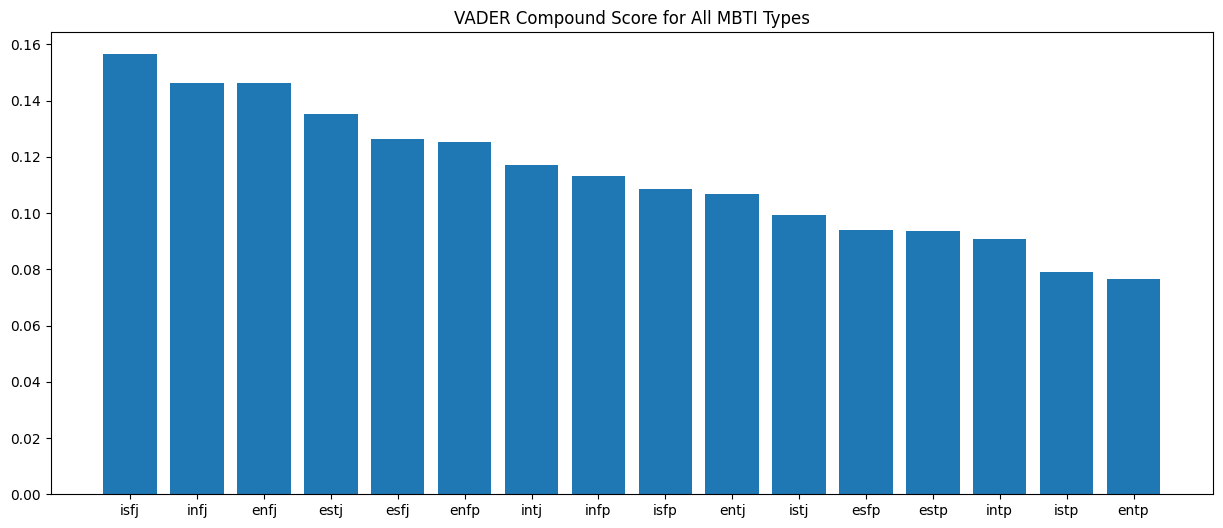
\includegraphics[width=0.3\textwidth]{Q2VADER1} 
		\caption{Cleaned Data printed out}		
	\end{figure}
	
	\subsubsection{Linguistic Style Patterns of MBTI Types}
	We select 4 distinct linguistic dimensions to represent linguistic styles:
	\begin{enumerate}
		\item Sentence Quantity: A larger sentence quantity suggests that the
		user tends to express themselves in shorter, more frequent statements.
		This may reflect a conversational, spontaneous communication style,
		often associated with extraversion or emotional openness.  
		\item Word Count: Higher word count may indicate a more elaborative or
		expressive communication habit, suggesting the user tends to provide
		more context or detail. This could reflect traits such as
		thoughtfulness, emotional depth, or even analytical thinking.
		\item Upper-Case Ratio: A higher ratio of uppercase letters often
		signifies stronger emotional expression, emphasis, or a more dramatic
		tone. It may reveal higher emotional arousal or a more assertive
		communication style, which could be linked to personality traits like
		enthusiasm or dominance. %e reading ease maybe only one coefficient
		\item Reading Ease(reflected by both Flesch and GF index): Higher reading
		ease scores imply simpler sentence structures and more familiar
		vocabulary, often seen in casual or informal communication. In contrast,
		lower scores suggest complexity and abstractness, which could indicate
		intellectual engagement, formality, or introversion. In our project, we
		adopted two kinds of rating systems to evaluate the reading ease of a
		context. The higher the Flesch Reading Ease score is, the easier the
		context can be understood; the lower the GF index is, the easier the
		context can be understood.
	\end{enumerate}
	
	These values are first computed before further analysis.
	\begin{enumerate}
		\item Class Definition \& Constructor
		\begin{python}
class Data_to_Analyze(Data_to_Clean):
    def __init__(self, type, source=raw_data):
        super().__init__(source)
        self.data = self.data.loc[self.data["type"] == type].reset_index(drop=True)
        self.data_to_vec = None
        self.basic_identities = pd.Series({
            "type": type,
            # Number of sentences in a post
            "sentence_quantity": [],
            "ave_sentence_quantity": None,
            # Number of words in a post
            "word_count": [],
            "ave_word_count": None,
            # Ratio of upper case characters in a post
            "upper_ratio": [],
            "ave_upper_ratio": None,
            # Two readability indicators: Flesch Reading Ease and Gunning Fog Index
            "reading_ease": [],
            "ave_reading_ease": None,
            "GF_index": [],
            "ave_GF_index": None,
            # Overall sentiment indicator (VADER)
            "overall_vader_score": None
        })

		\end{python}
		Defines a class \texttt{Data\_to\_Analyze} that inherits from \texttt{Data\_to\_Clean}.
		\begin{itemize}
			\item \textbf{Data subset} – The constructor calls
			super().\_\_init\_\_(source) to initialize the parent class, then
			filters the dataset so that only rows whose type column equals the
			target MBTI type remain (self.data).
			\item \textbf{Feature container} – basic\_identities is a pd.Series
			used to store a collection of text statistics: sentence count, word
			count, upper case ratio, readability metrics (Flesch Reading Ease
			and Gunning Fog Index) and an overall VADER sentiment score.
		\end{itemize}
		\item Sentence Count
		\begin{python}
def get_sentence_quantity(self):
    for post in self.data["posts"].values:
        self.basic_identities["sentence_quantity"].append(len(post))
    self.basic_identities["ave_sentence_quantity"] = ave(self.basic_identities["sentence_quantity"])
		\end{python}
		
		Iterates through every post (each post is already a list of sentences).
		The length of the list gives the number of sentences, which is appended
		to \texttt{sentence\_quantity}. Finally, the helper \texttt{ave()} computes their mean.
		\item Word Count
		\begin{python}
def get_word_count(self):
    for post in self.data["posts"].values:
        total = 0
        for sentence in post:
            total += len(sentence.split(" "))
        self.basic_identities["word_count"].append(total)
    self.basic_identities["ave_word_count"] = ave(self.basic_identities["word_count"])
		\end{python}
		
		For each post, it splits every sentence on whitespace to count words and
		sums them into total. The total per post is stored in \texttt{word\_count}, and
		the average is calculated afterwards.
		\item Upper Case Character Ratio
		\begin{python}
def get_upper_ratio(self):
    for post in self.data["posts"].values:
        char_count = 0
        upper_count = 0
        for sentence in post:
            for ch in sentence:
                if ch.isalpha():
                    char_count += 1
                    if ch.isupper():
                        upper_count += 1
        if char_count:
            self.basic_identities["upper_ratio"].append(upper_count / char_count)
    self.basic_identities["ave_upper_ratio"] = ave(self.basic_identities["upper_ratio"])
		\end{python}
		
		Traverses every character of every sentence, counting alphabetic
		characters (\texttt{char\_count}) and, among them, the upper case ones
		(\texttt{upper\_count}). The ratio per post is stored; the overall mean is then
		computed.
		\item Readability Metrics
		\begin{python}
def get_readability(self):
    reading_ease = []
    GF_idx = []
    for post in self.data["posts"].values:
        concatenated = post[0]
        for idx in range(1, len(post)):
            concatenated += post[idx]
        reading_ease.append(textstat.flesch_reading_ease(concatenated))
        GF_idx.append(textstat.gunning_fog(concatenated))
    self.basic_identities["reading_ease"] = reading_ease
    self.basic_identities["ave_reading_ease"] = ave(reading_ease)
    self.basic_identities["GF_index"] = GF_idx
    self.basic_identities["ave_GF_index"] = ave(GF_idx)
		\end{python}
		
		Each post’s sentences are concatenated into a single string, after which
		textstat computes Flesch Reading Ease and Gunning Fog Index. Both per
		post values and their averages are stored.
		%e 文字格式不对
	\end{enumerate}
	
	The calculation results are printed and displayed.
	\begin{python}
mbti_identities={
    T.upper():{
        k:cleaned_data[T].basic_identities[k]
        for k in [
        "ave_sentence_quantity",
        "ave_word_count",
        "ave_upper_ratio",
        "ave_reading_ease",
        "ave_GF_index"
        ]
    }
    for T in MBTI_types
}
mbti_identities=pd.DataFrame(mbti_identities).T
mbti_identities
	\end{python}
	\begin{figure}[H]
		\centering
		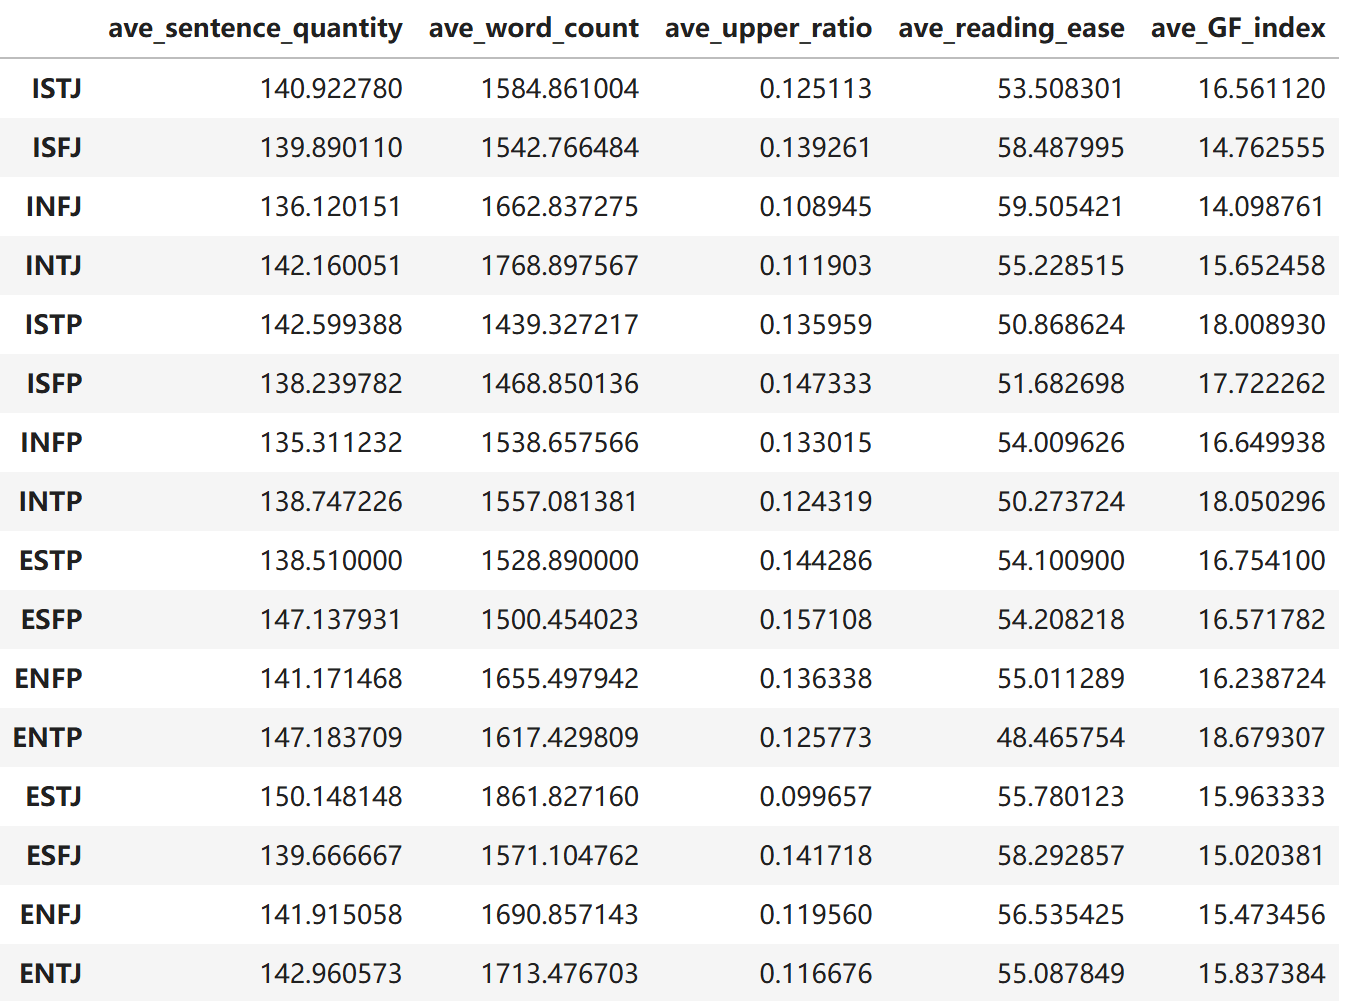
\includegraphics[width=0.9\textwidth]{Q2wordchart} 
		\caption{Table of Linguistic Style Features of MBTI Social Media Posts}		
	\end{figure}
	
	In order to better interpret the underlying patterns in the table, we
	present descending histograms for visual analysis.
	\begin{python}
column_mapping={
    "ave_sentence_quantity":"Sentence Quantity",
    "ave_word_count":"Word Count",
    "ave_upper_ratio":"Upper Case Letter Ratio",
    "ave_reading_ease":"Reading Ease"
}
fig,axes=plt.subplots(2,2,figsize=(18,10))
axes=axes.flatten()
for i,col in enumerate(mbti_identities.columns[:4]):
    axes[i].bar(mbti_identities[col].sort_values(ascending=False).index, mbti_identities[col].sort_values(ascending=False))
    axes[i].set_ylabel(f"{column_mapping[col]}")
    axes[i].set_title(f"{column_mapping[col]}")
fig.suptitle("Linguistic Features of MBTI Social Media Posts",fontsize=14, fontweight='bold')
plt.legend()
plt.tight_layout()
plt.savefig("final_output/ling_features.png")
plt.show()
	\end{python}
\begin{figure}[H]
    \centering
    \adjustbox{max width=1.2\textwidth,center}{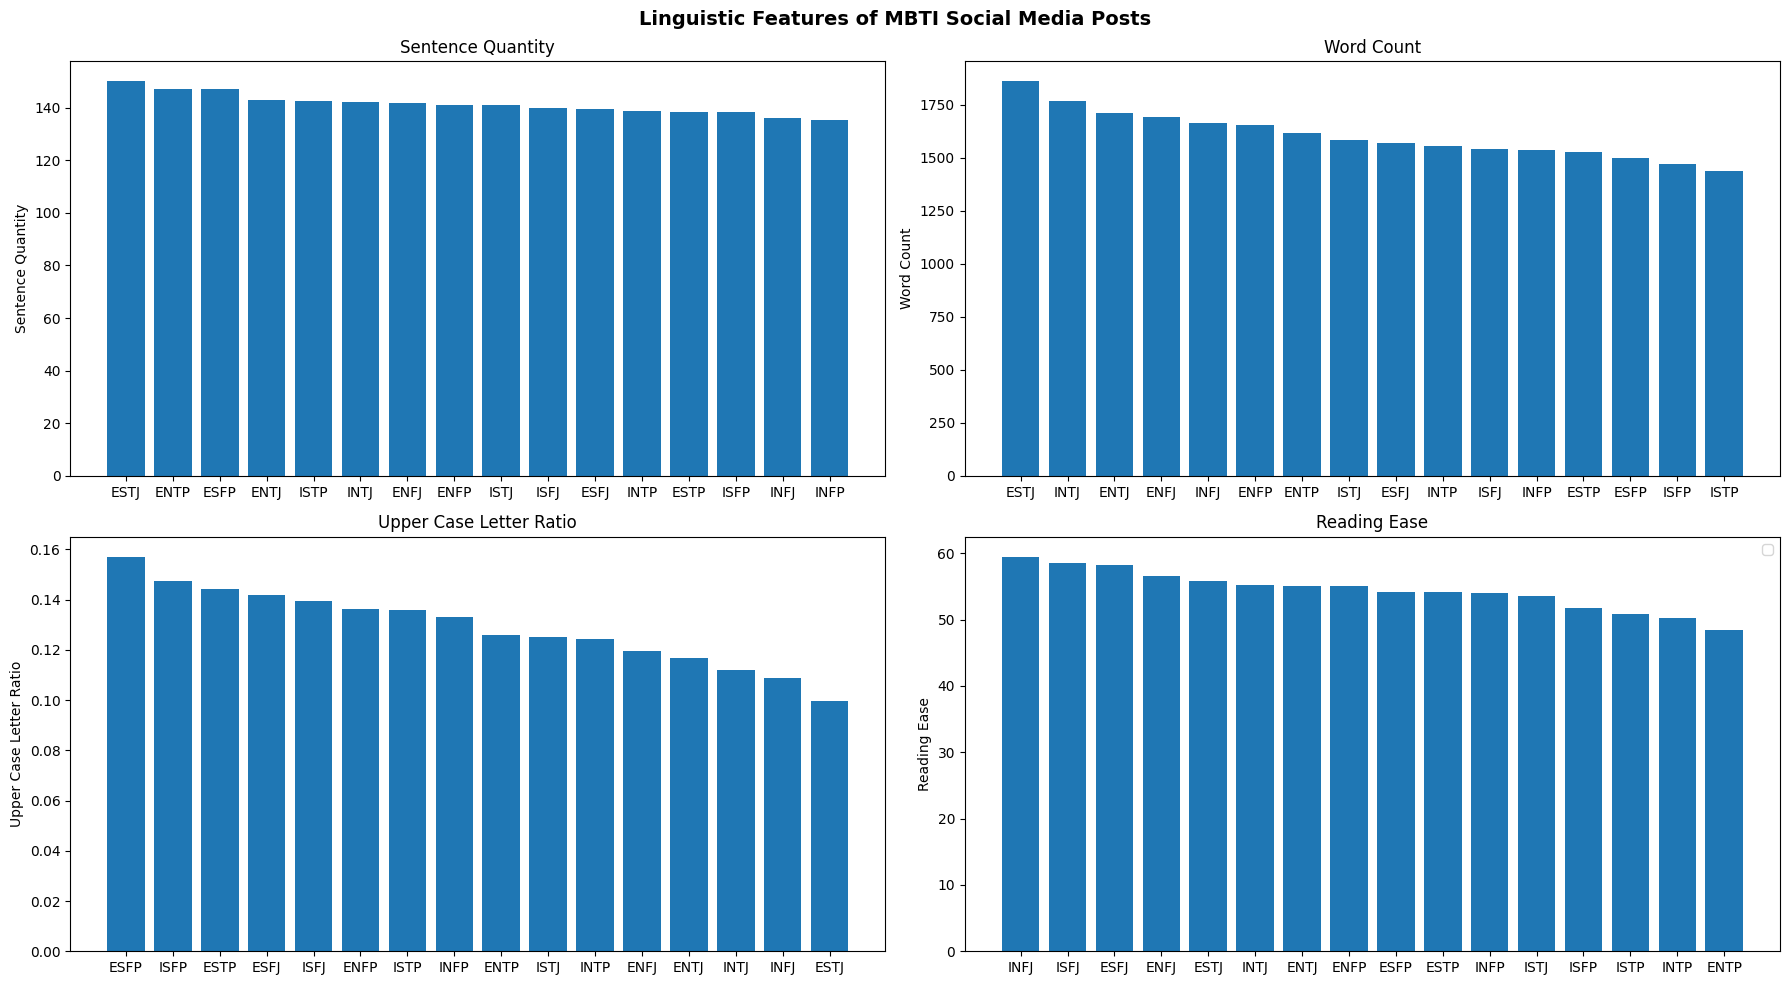
\includegraphics{Q2wordplot}}
\end{figure}
	The histograms allow the observation of surface-level patterns in linguistic styles.
	\begin{enumerate}
	\item Sentence Quantity: The top three MBTI types with the highest average
	sentence counts are ESTJ (150.1), ENTP (147.2), and ESFP (147.1). In
	contrast, the bottom three are INFP (135.3), INFJ (136.1), and ISFJ (139.9).
	This may indicate a correlation between the Extroversion/Introversion type
	and the extent of verbal expression. However, the overall variation in
	sentence quantity is relatively minor, suggesting limited explanatory
	significance.
	\item Word Count: ESTJ leads with an average of 1,861.8 words per post,
	followed by INTJ (1,768.9) and ENTJ (1,713.5). On the other end, ISTP
	(1,439.3), ISFP (1,468.9) and ESFP (1,500.5) write the fewest words.
	Overall, Thinking-Judging types (TJs) consistently post at greater length
	than Perceiving-Feeling types (PFs)
	\item Upper-Case Ratio:  Posts by ESFP (15.7\% uppercase), ISFP (14.7\%),
	and ESTP (14.4\%) contain the highest proportion of capital letters, whereas
	ESTJ (10.0\%), INFJ (10.9\%), and INTJ (11.2\%) post the least.
	Feeling-Perceiving personalities prefer to use uppercase—perhaps as a tool
	for emphasis or emotional expression—while Thinking-Judging profiles favor a
	more uniform casing. 
	\item Reading Ease: On the Flesch scale, INFJ (59.5), ISFJ (58.5), and ESFJ
	(58.3) write the most readable posts, whereas ENTP (48.5), INTP (50.3), and
	ISTP (50.9) produce denser, more complex text. Judging-Feeling types tends
	for simpler, clearer phrasing, while Perceiving-Thinking types trend toward
	more intricate language.
	\end{enumerate}
	
	Three characteristic can also be observed from the standpoint of MBTI types.
	\begin{enumerate}
	\item ESTJ exhibits the greatest information throughput—leading all types in
	both mean sentence count and mean word count—whereas ENTP, although nearly
	as verbose in sentence frequency, records the lowest readability and most
	negative sentiment, underscoring that sheer output does not translate into a
	warmer tone.
	\item ESFP and ISFP personalities stand out for their high upper-case
	ratios, corresponding to the commonly held view of ‘FP’ types as spontaneous
	and emotionally guided.
	\item INFJ produces the most readable texts. Meanwhile, they are also among
	the top three most positive in emotional expression(analyzed in the next
	section). ENTP produces the least readable and positive texts.

	\end{enumerate}
	 
	
	
	
	\subsubsection{Sentiment Analysis}
	Sentiment analysis, or opinion mining, is an active area of study in the
	field of natural language processing that analyzes people's opinions,
	sentiments, evaluations, attitudes, and emotions via the computational
	treatment of subjectivity in text. There are various approaches to
	sentimental analysis. In this assignment, we choose VADER(Valence Aware
	Dictionary for sEntiment Reasoning) as our tool to analyze the difference of
	different MBTI personalities in emotional expression due to its superiority
	in social media context\cite{VADER}.
	
	%VADER uses a pre-constructed system of "lexicon + weighted rules" to score each word in the input text and generate an overall sentiment score. For every given text, VADER first separates the text into words. Then, it rates the words from -4 to 4(4 as the most positive, and -4 as the most negative) according to its 7,500-entity valence lexicon. To increase the rating accuracy and distinguish between strength of emotions, VADER corrects the scores with a set of rules, which includes increasing or decreasing the score when identifying capitalization, negative and contrastive words. The details rating process is represented in the flow chart below.
	%插入图片
	
	We do the following steps to acquire VADER scoring:

	 \begin{python}
analyzer = SentimentIntensityAnalyzer()
overall_vader_score = {'neg': 0.0, 'neu': 0.0, 'pos': 0.0, 'compound': 0.0}
	\end{python}
	\begin{itemize}
	\item Instantiate NLTK’s SentimentIntensityAnalyzer to compute sentiment
	scores.
	\item Initialize overall\_vader\_score as an aggregate dictionary with the
	four sentiment components (neg, neu, pos, compound), which will be used to
	assess the text’s overall emotional state.

	\end{itemize}

	\begin{python}
def addup_score_dict(new_dict, base_dict):
    for key in base_dict.keys():
        base_dict[key] += new_dict[key]
	\end{python}
	This function adds the sentiment scores of a sentence (or post) to the
	target dictionary. It iterates over the keys and sums the corresponding
	values, allowing either local or global sentiment accumulation.

	\begin{python}
def process_vader_score(post):
    post_vader_score = {'neg': 0.0, 'neu': 0.0, 'pos': 0.0, 'compound': 0.0}
    for sentence in post:
        addup_score_dict(analyzer.polarity_scores(sentence), base_dict=post_vader_score)
    ave_score_dict(base_dict=post_vader_score, n=len(post))
    addup_score_dict(new_dict=post_vader_score, base_dict=overall_vader_score)
    return post_vader_score
	\end{python}
	This nested function analyzes the sentiment of a single post (a list of
	sentences) through the following steps:
	% 或许还是画一个图?
	\begin{enumerate}
	\item Initialize a score container for the post.
	\item Traverse each sentence and obtain its sentiment scores with
	polarity\_scores().
	\item Accumulate the sentence scores and divide by the number of sentences
	to compute the post’s average sentiment.
	\item Add this post’s average score to the overall accumulator
	overall\_vader\_score.
	\item Return the post’s sentiment score so it can be stored back in the
	dataset.
	\end{enumerate}
	\begin{python}
self.data["vader_score"] = self.data["posts"].apply(process_vader_score)
	\end{python}
	This line applies process\_vader\_score to every post in self.data. The
	returned score dictionaries (neg, neu, pos, compound) are stored in a new
	column named vader\_score.
	\begin{python}
ave_score_dict(overall_vader_score, len(self.data["posts"]))
self.basic_identities["overall_vader_score"] = overall_vader_score
	\end{python}
	After accumulating all post-level scores into overall\_vader\_score, divide
	by the total number of posts to obtain the average sentiment. Finally,
	record this overall score in the basic\_identities dictionary under the key
	"overall\_vader\_score" as the global emotional characteristic of the
	personality type.
	
	Having acquired the VADER score, we collect the average sentiment into a
	chart that is ordered by descending compound score.
	\begin{python}
all_vader_scores={T:cleaned_data[T].basic_identities["overall_vader_score"] for T in MBTI_types}
all_vader_scores=pd.DataFrame(all_vader_scores).T
all_vader_scores=all_vader_scores.sort_values(by="compound",ascending=False)
all_vader_scores
	\end{python}
	\begin{figure}[H]
			\centering
			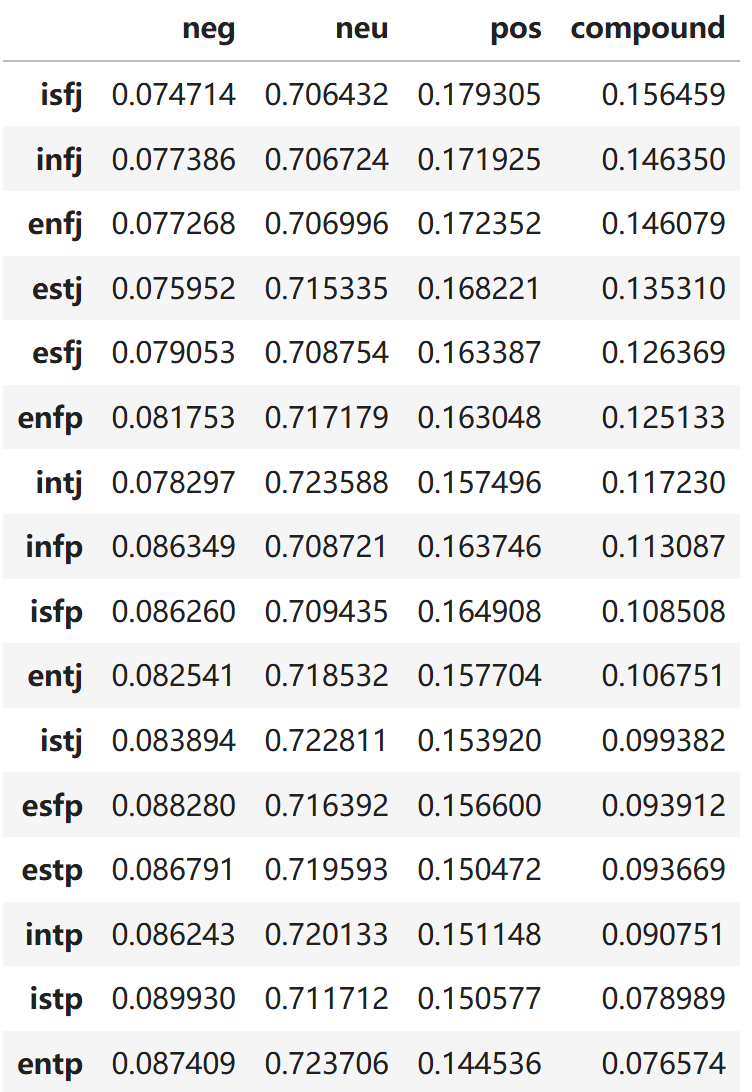
\includegraphics[width=0.5\textwidth]{Q2VADERSCORE} 
			\caption{\centering Negative, Neutral, Positive and Compound VADER Score arranged in descending compound order}		
	\end{figure}
	The characteristics of compound VADER score is described.
	\begin{python}
all_vader_scores["compound"].describe()
	\end{python}
	\begin{figure}[H]
			\centering
			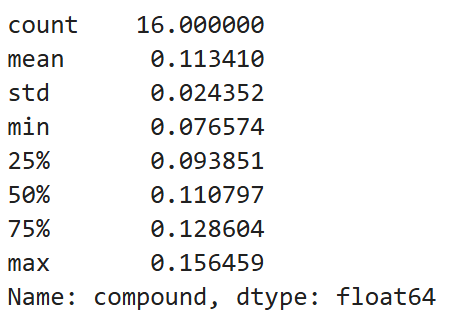
\includegraphics[width=0.5\textwidth]{Q2CV} 
			\caption{\centering Description of Compound VADER Scores}		
	\end{figure}
	
	From the description, we find that the standard deviation is approximately
	0.0243, showing a small overall fluctuation. The range between the most and
	least positive types spans about 3.3σ, indicating a significant but not
	extreme variation. Additionally, the standard deviation accounts for only
	about 20\% of the mean, implying a compact and smooth distribution.
	
	The fact that mean is slightly greater than the median suggests a longer
	tail on the higher end of the scale, which indicates that the distribution
	exhibits a slight right skew, towards a positive emotional expression. This
	is supported by a having positive mean value(0.113).
	
	We further visualized the compound results of different MBTI by descending
	order to find the relationship of MBTI personalities and their sentimental
	expression.
	
	\begin{python}
x=all_vader_scores.index
y=all_vader_scores["compound"]
plt.figure(figsize=(10, 6))
plt.bar(x,y)
plt.xlabel("MBTI Types")
plt.ylabel("VADER Compound Score")
plt.title("VADER Compound Score for All MBTI Types",fontsize=14, fontweight='bold')
plt.tight_layout()
plt.savefig("final_output/vader.png")
plt.show()
	\end{python}
	\begin{figure}[H]
			\centering
			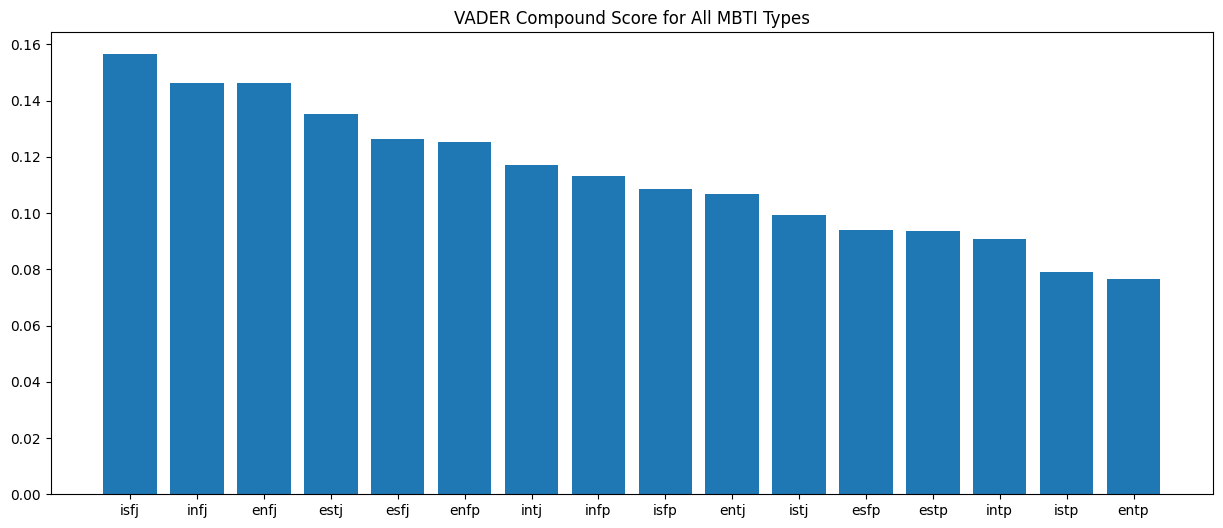
\includegraphics[width=1\textwidth]{Q2VADERa1} 
			\caption{\centering }		
	\end{figure}
	
	We find that ISFJ, INFJ, ENFJ has the highest compound score, while ISTP,
	ENTP has the lowest, suggesting personalities with F and J tend to be more
	positive in emotional expression.
	
	To verify this point, we first decomposed every personality label into its
	four constituent letters and collected all VADER-compound scores belonging
	to the same pole of a dichotomy.  If
	$D\in\{\text{I/E},\text{S/N},\text{T/F},\text{J/P}\}$ and $L$ denotes one
	pole of $D$ (e.g., $L=\text{F}$ within $D=\text{T/F}$), the group mean is
	obtained by
	
	$$
	\bar{x}_{L}=\frac{1}{n_{L}}\sum_{k\in L}x_{k},
	$$
	
	where $x_{k}$ is the compound score of the $k$-th MBTI type and $n_{L}$ is
	the number of types that contain the letter $L$.  Letting
	
	$$
	\mu=\frac{1}{16}\sum_{i=1}^{16}x_{i}
	$$
	
	denote the grand mean across all sixteen personalities, we express the
	relative contribution of letter $L$ as
	
	$$
	\Delta_{L}= \frac{\bar{x}_{L}-\mu}{\mu}\times100\%.
	$$
	
	Applying these definitions to our data we obtain
	$\bar{x}_{\text{F}}=0.126987$, $\bar{x}_{\text{T}}=0.099832$,
	$\bar{x}_{\text{J}}=0.129241$, and $\bar{x}_{\text{P}}=0.097578$, while the
	grand mean is $\mu=0.113410$.  Consequently, Feeling exceeds Thinking by
	$\Delta_{\text{F,T}}\approx 23.9\%$ and Judging exceeds Perceiving by
	$\Delta_{\text{J,P}}\approx 31.6\%$, whereas the contrasts for
	Extraversion–Introversion and Intuition–Sensing remain below 3 \%.  These
	magnitudes confirm that the third and fourth MBTI letters (T/F, J/P) play a
	significantly greater role in shaping positive emotional expression, while
	first two dimension make relatively small contribution.
	
	To find the relation between the four roles—Diplomats ( NF), Sentinels
	( SJ), Analysts ( NT) and Explorers ( SP)—we test its relative contribution.
	Writing $G\in\{\text{NF},\text{SJ},\text{NT},\text{SP}\}$ and letting
	$n_{G}$ be the number of types in group $G$ $(n_{G}=4)$, the group score is
	obtained by
	
	$$
	\bar{x}_{G}= \frac{1}{n_{G}}\sum_{k\in G}x_{k},
	\qquad
	G\in\{\text{NF},\text{SJ},\text{NT},\text{SP}\},
	$$
	
	with the grand mean $\mu$ defined in equation above.  Substituting the
	individual compound values yields
	
	$$
	\bar{x}_{\text{NF}} = 0.133,\qquad 
	\bar{x}_{\text{SJ}} = 0.129,\qquad
	\bar{x}_{\text{NT}} = 0.098,\qquad
	\bar{x}_{\text{SP}} = 0.094 .
	$$
	
	To place these figures on the common scale used earlier, we again report the
	relative deviation
	
	$$
	\Delta_{G}= \frac{\bar{x}_{G}-\mu}{\mu}\times 100\% .
	$$
	
	Hence
	
	$$
	\Delta_{\text{NF}}=+17.3\%,\quad 
	\Delta_{\text{SJ}}=+13.7\%,\quad
	\Delta_{\text{NT}}=-13.6\%,\quad
	\Delta_{\text{SP}}=-17.1\%.
	$$
	
	The ranking $\bar{x}_{\text{NF}}>\bar{x}_{\text{SJ}}>\bar{x}_{\text{NT}}>\bar{x}_{\text{SP}}$ mirrors the earlier letter-level findings: Diplomats, combining the affective “F’’ and the future-oriented “N’’, produce the warmest tone; Sentinels follow closely, driven by the strongly positive “J’’ component; Analysts, dominated by the critical “T’’, adopt a noticeably cooler register; and Explorers, whose “P’’ preference and playful spontaneity encourage criticism and slang, exhibit the lowest positivity. 
	


	
	

	\begin{python}
def get_sentence_quantity(self):
    for post in self.data["posts"].values:
        self.basic_identities["sentence_quantity"].append(len(post))
    self.basic_identities["ave_sentence_quantity"] = ave(self.basic_identities["sentence_quantity"])
	\end{python}
	
\section{Conclusion}	
Together, these two strands of evidence allow us to adopt a dialectical stance: 
MBTI’s four dimensions yield reliable behavioral insights, yet its theoretical assumption of strict independence does not fully hold. 
In other words, MBTI remains a valuable framework—provided its limitations are recognized and its results interpreted with appropriate caution.

On the one hand, according to Pittenger (1993), \textit{“we would expect each factor to be independent of the other factors, inasmuch as the MBTI theory states that each of the four preference dimensions stands alone;
 questions within one factor should not correlate with questions in the other factors” }(p. 50). However, our empirical tests contradict this assumption: both chi-square analyses and inter-factor correlation matrices reveal that the four MBTI dimensions—E–I, S–N, T–F, and J–P—are not statistically independent, calling into question the theoretical orthogonality upon which MBTI is predicated.

MBTI can play a valuable role in facilitating self-awareness, improving team communication, and guiding career exploration by highlighting broad preference tendencies. It offers a common language for discussing interpersonal differences and can inform coaching, leadership development, and collaborative problem-solving. However, relying too heavily on MBTI carries risks. First, type labels can become “social tags” that oversimplify complex inner worlds and foster stereotypes—for example, assuming every INTJ is cold and rational ignores their potential for empathy and emotional depth. Second, the reliability of any single test result is limited by mood, stress, social-desirability bias, and the test-taker’s context; using one score to choose friends or partners lacks scientific support. Finally, excessive trust in MBTI can open the door to manipulation, as bad actors may exploit type labels to gain trust or social leverage.

In short, MBTI offers valuable directional insight into broad personality tendencies—serving as a springboard for personal growth, team building, and career conversations—but it should never be the sole yardstick for judging an individual. By recognizing its psychometric limitations, avoiding type-based stereotypes, and remaining alert to potential misuse, we can benefit from MBTI’s strengths while steering clear of the pitfalls of oversimplified personality labelling.

% ----------------- References ------------------------------
	\bibliographystyle{apacite}
	\bibliography{references}

\end{document}
